\newpage % Zaleca się otwieranie rozdziału od nowej strony.
\section{Wstęp}

\textbf{Rozpoznawanie mowy} jest techniką umożliwiającą systemom komputerowym interpretowanie ludzkiej mowy, na przykład w~celach transkrypcji lub jako alternatywną metodę interakcji \cite{Wiki:Speech}.
Umożliwia to komunikację między komputerem a~człowiekiem w~sposób bardziej naturalny niż przy użyciu standardowych interfejsów użytkownika. Dla człowieka intuicyjniejsze jest wydawanie poleceń głosem niż za pomocą przycisków. Mówienie jest naturalną formą komunikacji człowieka ze środowiskiem, a~jego interpretacja w~urządzeniu czyni je bardziej wygodnym w~użytkowaniu \cite{Elektronika:Speech}.

Ludzie interesują się \textbf{rozpoznawaniem mowy} już od co najmniej setek lat, jednak dopiero w~połowie XX wieku udało się stworzyć technikę, która rozpoznawała ludzki głos z~satysfakcjonującą precyzją. Pierwszym takim projektem był \textit{Audrey}, system stworzony w~\textit{Bell Laboratories} w~1952 roku, pozwalający na rozpoznawanie wymawianych cyfr od 0 do 9. Następnie pojawiły się projekty rozwijające tę koncepcję, na przykład \textit{Shoebox}, który dodatkowo rozpoznawał nazwy operacji matematycznych. Zastosowano nowe techniki, takie jak ukryte modele Markowa (HMM) czy technika \textit{MFCC}. Ze względu na losowość sygnału mowy wprowadzono techniki sztucznej inteligencji, takie jak sieci neuronowe. W~latach 90. pojawiły się pierwsze komercyjne urządzenia umożliwiające rozpoznawanie mowy nie tylko w~warunkach laboratoryjnych \cite{Transcribe:Speech}.

Dziś coraz większa liczba urządzeń umożliwia interakcje za pomocą systemów rozpoznawania mowy (\textit{ASR}), co pozwala producentom sprzętu na dodawanie nowych funkcji, czyniąc ich produkt bardziej atrakcyjnym dla użytkownika końcowego.

Urządzenia pozwalające na sterowanie głosem spełniają coraz bardziej restrykcyjne wymagania. Obecnie potrafią rozpoznawać wypowiedzi w~środowisku mocno zaszumionym, z~obcymi dźwiękami w~tle, takimi jak odgrywana muzyka. Algorytmy te stają się coraz szybsze, często wykorzystuje się układy wspomagające \textit{DSP} (Digital Signal Processing), które dzięki możliwości zwielokrotnienia operacji w~czasie, przyspieszają przetwarzanie mowy. Ponadto używa się układów wspomagających sztuczną inteligencję, niezależnie od użytego algorytmu. Można również wykorzystać karty graficzne w~komputerach, co znacznie skraca czas wykrywania słów, co sprawia, że interfejs jest mniej irytujący podczas użytkowania. Podobnie wzrasta odporność takich systemów na różnorodność mowy ludzkiej, wliczając wady wymowy. W~latach 90., gdy pojawiały się pierwsze komercyjne rozwiązania rozpoznające mowę, użytkownik musiał mieć bardzo dobrą dykcję. Dzisiaj systemy te są znacznie bardziej tolerancyjne, a~współczesny próg komercyjnej akceptowalności systemów rozpoznawania mowy zwykle przyjmuje się jako 95\% poprawności rozpoznania~\cite{Ziolko:Speech}.

Jednak systemy te mają zasadniczą wadę. Urządzenia, szczególnie te o~mniejszych zasobach, takie jak inteligentne głośniki, często wysyłają nagrania lub metadane do chmury~\cite{JBL:Support} lub mają ograniczoną funkcjonalność~\cite{Google:Support}. Powoduje to liczne obawy o~prywatność, gdyż urządzenia te mogą teoretycznie służyć do podsłuchiwania ludzi. Nie ma pewności, mimo różnych polityk prywatności, czy producent nie łamie ich niejawnie~\cite{Google:Privacy}.

Rozwój technologii oraz podłączanie coraz większej liczby urządzeń do sieci spowodowało powstanie zjawiska zwanego \textit{Internetem Rzeczy}. Coraz więcej urządzeń jest podłączonych do sieci nie tylko na potrzeby sztucznej inteligencji czy rozpoznawania mowy, ale także do zbierania innych danych, np. statystycznych. Pozwala to na przetwarzanie danych na urządzeniach o~większej mocy obliczeniowej, aby np. użyty w~danym miejscu czujnik nie zajmował dużo miejsca i~nie pobierał niepotrzebnie dużo energii. Rozwiązania te najczęściej korzystają z~łączności bezprzewodowej, co pozwala na efektywniejsze zarządzanie dużymi instytucjami.

Systemy \textbf{IoT}, z~uwagi na małą moc obliczeniową węzłów, często ograniczają się jedynie do zbierania prostych danych z~czujników. Czasem jednak to niewystarczające dla pełnego zbierania informacji z~otoczenia. W~ten sposób może powstać potrzeba, aby w~danym miejscu wykrywać mowę, a~przynajmniej pojedyncze wyrazy. Jest to proces niewymagający zaawansowanego rozpoznawania mowy ciągłej itp., co może poszerzyć ilość informacji zbieranych przez dany system \textit{Internetu Rzeczy}, zwiększając jego funkcjonalność, która jest niedostępna dla prostych systemów czujnikowych, szczególnie tam, gdzie potrzebna jest interakcja z~człowiekiem, np. zbieranie żądań od osób przebywających w~danym pomieszczeniu.

Urządzenia umożliwiające obecnie taką funkcjonalność, możemy podzielić na zależne od mówiącego (\textit{speaker dependent}) oraz niezależne od niego (\textit{speaker independent}). Systemy te nie wymagają kooperacji z~chmurą przy samym procesie wykrywania wyrazów, mają bardzo ograniczoną liczbę słów, jakie mogą wykrywać, tylko te związane z~funkcjonalnościami danego systemu. Wymagają niewiele pamięci, a~wraz z~postępem technicznym, ich jakość wykryć jest porównywalna z~uzyskiwaną przez zaawansowane chmurowe asystenty mowy~\cite{LED:Speech}.

\subsection{Cele pracy}

Głównym celem tej pracy będzie stworzenie prototypu \textbf{węzła IoT, który rozpoznawałby proste rozkazy}, ale również zachowałoby prywatność, ograniczając ilość danych wyłącznie do pojedynczych rozkazów w~ściśle określonym słowniku. Słownik ten byłby dopasowany do konkretnego miejsca, w~którym urządzenie byłoby użyte (na przykład węzeł umożliwiający sterowanie roletami w~pokoju, gdzie jego funkcjonalność ogranicza się do dwóch poleceń: \textit{góra} — po którym rolety są podnoszone oraz \textit{dół} — są one opuszczane).

Uniemożliwiłoby to przechwycenie wrażliwych informacji. Informacja o~wykrytym rozkazie byłaby następnie przesyłana za pomocą interfejsu bezprzewodowego do dalszego przetworzenia — w~tej pracy będzie to technika \textit{Bluetooth Low Energy}. Urządzenie to byłoby niezależne od osoby mówiącej (\textit{speaker independent}). Operacje wykonywane przez to urządzenie wymagają dedykowanej akceleracji sprzętowej, aby uzyskać detekcję słów w~rozsądnym czasie, dlatego wykorzystano do budowy tego węzła FPGA, co umożliwia implementację specjalizowanego chipu w~warunkach nielaboratoryjnych.

Realizację powyższego celu można rozpisać na mniejsze cele wymienione poniżej.
\begin{itemize}
	\item opracowanie dedykowanej metody rozpoznawania mowy przy użyciu narzędzi otwartoźródłowych, dostosowanej do małych zasobów pamięciowych oraz do rozpoznawania mowy bez potrzeby przesyłania nagrania lub metadanych do chmury.
	\item zaprojektowanie implementacji sprzętowo-programowej wspomnianego wyżej sposobu.
	\item stworzenie kompletnego \textit{SoC} (System on a~Chip), będącego głównym procesorem projektowanego węzła \textit{IoT}, wykorzystującego wspomnianą implementację, umożliwiającego komunikację ze światem zewnętrznym — odbieranie dźwięków i~komunikacja bezprzewodowa.
	\item opracowanie uniwersalnej platformy na potrzeby stosowania sztucznej inteligencji w~urządzeniach wbudowanych (\textit{embedded}).
	\item opisanie metod weryfikacji części sprzętowej na podstawie narzędzi dostarczonych przez producenta platformy docelowej, uwzględniając zarówno aspekty sprzętowe, jak i~programowe.
	\item testy projektowanego \textit{SoC} jako głównego procesora docelowego urządzenia rozpoznającego mowę w~naturalnym środowisku pracy węzła \textit{IoT}.
	\item ocena rozwiązania pod względem precyzji wykrywania rozkazów, efektywności obliczeń oraz porównanie z~innymi podobnymi rozwiązaniami.
\end{itemize}


\newpage
\section{Stan wiedzy}

\subsection{Odbiór sygnału mowy}

Aby móc przetwarzać sygnał mowy, należy go najpierw odpowiednio przechwycić. Nagranie uzyskane przez mikrofon musi zostać przetworzone, aby było użyteczne podczas przetwarzania. Istotne jest określenie zakresu częstotliwości, które są słyszalne dla ludzkiego ucha. Przyjmuje się, że zakres ten wynosi dla samogłosek od 250 do 2000 Hz, a~dla samogłosek dźwięcznych (b, d, m, itd.) od 250 do 4000 Hz. Częstotliwość samogłosek bezdźwięcznych (f, s, t, itd.) mieści się w~przedziale od 2000 do 8000 Hz~\cite{ecophon:speech}. Słyszalność poszczególnych częstotliwości w~zależności od ich natężenia przedstawia wykres na rysunku 2.1.

\begin{figure}[h]
	\centering
	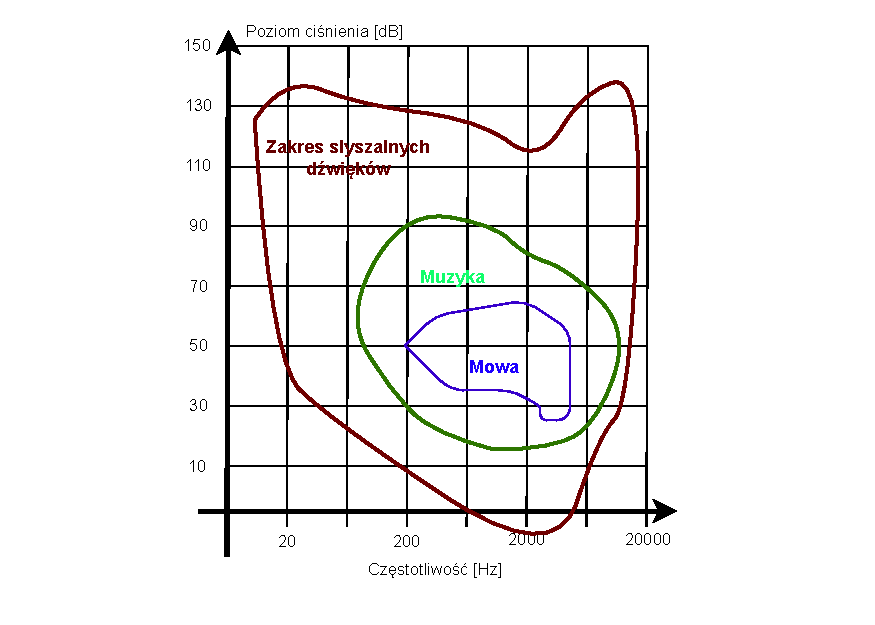
\includegraphics[width=0.9\textwidth]{Ucho.pdf}
	\caption{Zakres dźwięków słyszalnych dla ludzkiego ucha w~zależności od ich częstotliwości i~poziomu natężenia (ciśnienia)~\cite{DzwiekiUcho}}
\end{figure}
\FloatBarrier %zatrzymanie przenoszenia rysunku

Dźwięk odebrany przez mikrofon na potrzeby urządzeń cyfrowych jest zwykle rejestrowany z~częstotliwością 44 kHz lub 48 kHz~\cite{48}. Następnie, sygnał ten musi być odfiltrowany z~niepotrzebnych częstotliwości.

Urządzenia cyfrowe często używają filtru o~skończonej odpowiedzi impulsowej \textit{FIR}. Reakcja tego układu na pobudzenie jest skończonej długości. Filtry te nie posiadają pętli sprzężenia zwrotnego, co ilustruje rysunek 2.2~\cite{Wiki:FIR}.

\begin{figure}[h]
	\centering
	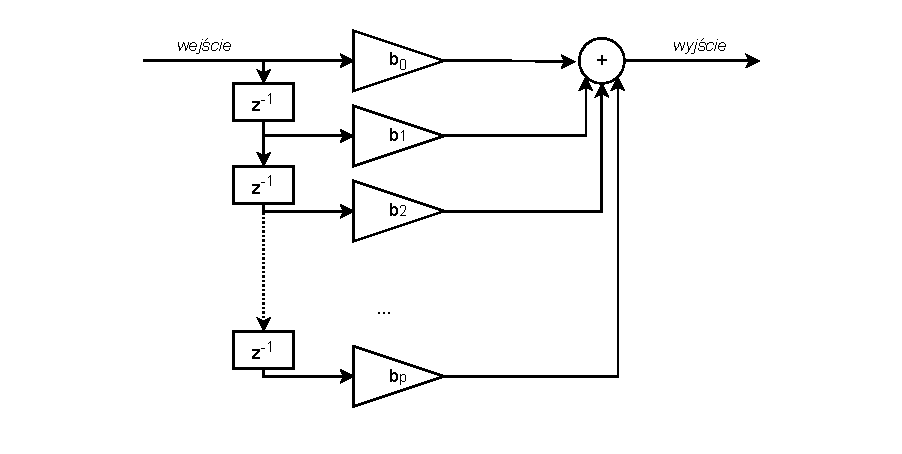
\includegraphics[width=1\textwidth]{filterS.pdf}
	\caption{Schemat filtru FIR~\cite{Wiki:FIR}.}
\end{figure}
\FloatBarrier %zatrzymanie przenoszenia rysunku

Realizowanie skomplikowanych transmitancji wymaga wielomianu wysokiego rzędu, dlatego, w~porównaniu z~filtrem o~nieskończonej odpowiedzi impulsowej, dla uzyskania podobnej charakterystyki potrzeba więcej zasobów sprzętowych~\cite{Wiki:FIR}. Im lepsze tłumienie danego pasma chcemy uzyskać, tym zazwyczaj wielomian będzie wyższego rzędu.

Filtry te mają prostą budowę, która pozwala na zrównoleglenie operacji. Zważywszy, że praca ta dotyczy implementacji systemu w~\textit{FPGA}, jest to cecha, która może być szczególnie interesująca~\cite{Wiki:FIR}. Po odpowiednim wytłumieniu zbyt wysokich częstotliwości można zmniejszyć częstotliwość próbkowania, standaryzując nagranie z~porównywanymi w~systemie, niezależnie od tego, czy jest to sieć neuronowa czy inny algorytm sztucznej inteligencji.


\subsection{Metody ekstrakcji cech mowy - MFCC}

Systemy rozpoznawania mowy obecnie opierają się głównie na sztucznej inteligencji. W~celu jej efektywnego działania należy oddzielić od nagrania dźwiękowego tylko te cechy (\textit{ekstrakcja cech}~\cite{Ekstrakcja}), które są pomocne w~prawidłowej detekcji wyrazów, eliminując szumy oraz obce dźwięki z~otoczenia.

Przed opracowaniem wstępnej koncepcji projektowanego systemu należało zebrać informacje o~metodach ekstrakcji cech dźwięku. Najczęściej stosowaną metodą dla rozpoznawania wyrazów jest \textbf{MFCC} - \textit{Mel-frequency Cepstrum}~\cite{Wiki:MFCC}.
\newpage
Algorytm ten zilustrowano na rysunku 2.3.

\begin{figure}[h]
	\centering
	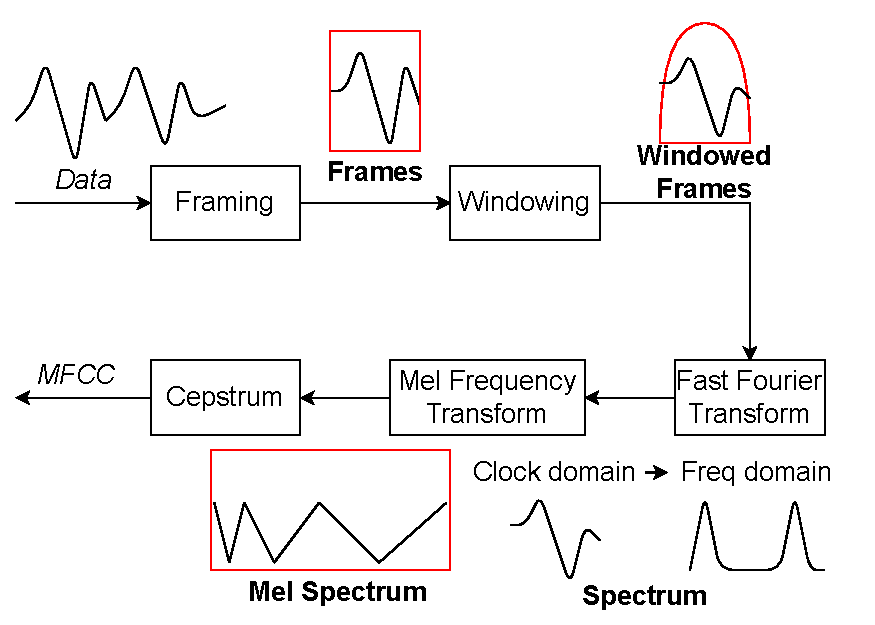
\includegraphics[width=0.7\textwidth]{MFCC.pdf}
	\caption{Ilustracja algorytmu \textit{MFCC}~\cite{MFCC:Rys}}
\end{figure}
\FloatBarrier %zatrzymanie przenoszenia rysunku

Operacja \textit{cepstrum} opiera się na transformacji Fouriera (\textit{spectrum}). Rezultatem jest przebieg pseudoczasowy, gdzie kolejne wartości na osi rzędnych można interpretować jako jednostki czasu, natomiast wartości na osi odciętych są w~pewien sposób związane z~autokorelacją, umożliwiając wyznaczenie tonu podstawowego~\cite{APD:PW}.

Podstawową operacją metody \textit{MFCC} jest szybka transformacja Fouriera (FFT). Jest to algorytm (przede wszystkim \textit{Cooleya-Tukeya}) \cite{CT:FFT}, który umożliwia efektywne obliczanie transformacji Fouriera za pomocą urządzeń cyfrowych \cite{Wiki:FFT}, zarówno układów cyfrowych, jak i~oprogramowania. Transformacja ta pozwala na zamianę sygnału z~dziedziny czasu na funkcję w~dziedzinie częstotliwości dla danego fragmentu sygnału poddanego \textit{próbkowaniu} \cite{Agh:Trans}. Operacja ta umożliwia określenie, które dźwięki (posiadające swoje charakterystyczne cechy) były dominujące. Wynik tej operacji nazywany jest \textit{widmem}.

Na początku sygnał jest poddawany ramkowaniu (\textit{frameing}), dzieli się go na krótkie fragmenty o~równej długości. Rozmiar ramek musi być wielokrotnością liczby 2, aby można było obliczać \textit{FFT}. Wielkość ramek musi być na tyle duża, aby uzyskana transformata miała odpowiednią precyzję w~dziedzinie częstotliwości, aby uniknąć uzyskania \textit{widma zgrubnego} \cite{Przetwarzanie}. Jednocześnie ramka musi być wystarczająco mała, aby nie stracić rozdzielczości czasowej \cite{PGFFT}.

Następnie, z~ramek obliczane jest okno czasowe (\textit{windowing}), które opisuje sposób pobierania próbek z~sygnału \cite{Wiki:FFT}. Pozwala to uniknąć tzw. zjawiska \textit{przecieku widma}, które pojawia się, gdy liczba cykli dla wyróżnionych w~sygnale składowych harmonicznych nie jest liczbą całkowitą. Powoduje to poszerzenie pików w~spektrogramie dla danych częstotliwości oraz większe listki boczne widma. Efekt ten jest niepożądany, gdyż nie odzwierciedla on rzeczywistego stanu \cite{Opolska:Przeciek}. Najczęściej stosowanym oknem wygładzającym, aby zapobiegać temu zjawisku, jest okno \textit{Hamminga}, które jest określone wzorem:

$$  w[n] = a~- b cos(\frac{2 \pi n}{N})$$


Gdzie $n$ to numer próbki w~ramce $a$ i~$b$ to współczynniki okna  (dla okna \textit{Hamminga} są to odpowiednio 0,53836 i~0,46164), a~$N$ jest rozmiarem okna. Aby uzyskać wartości próbek po przejściu przez okno, należy przemnożyć wartość okna dla danej próbki przez próbkę otrzymaną po ramkowaniu ($o[n] = w[n] r[n]$). Wpływ okna czasowego na sygnał ilustruje rys. 2.4.

\begin{figure}[h]
	\centering
	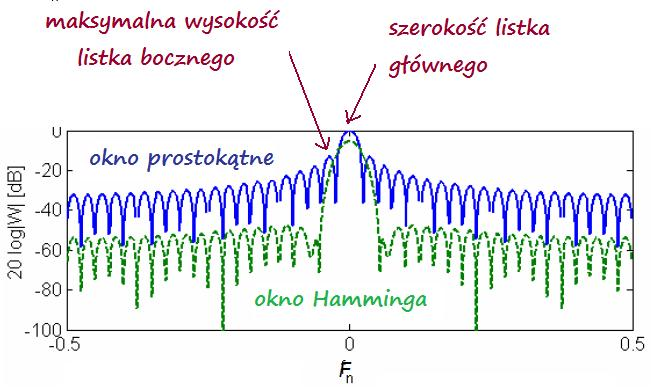
\includegraphics[width=0.6\textwidth]{hamm_prost.jpg}
	\caption{Porównanie widma sygnału dla okna prostokątnego i~okna \textit{Hamminga} \cite{AGH:Okna} - listki boczne są znacznie mniejsze niż dla prostokątnego odpowiednika}
\end{figure}

Następnie ustalone okna są poddawane transformacji Fouriera. Z~tej transformacji obliczany jest spektrogram, gdzie moc dla każdej uzyskanej częstotliwości obliczana jest poprzez obliczenie wartości bezwzględnej liczby zespolonej (transformacja Fouriera daje wynik w~dziedzinie liczb zespolonych).


\subsubsection{Skala melowa}

Ludzki słuch nie interpretuje częstotliwości dźwięków w~sposób liniowy. Niskie tony są przez człowieka rozróżniane precyzyjniej niż tony wysokie. Mając na uwadze tę zależność, opracowano tzw. \textit{skalę melową} (\textit{Mel Frequency Transform}) – skalę wysokości dźwięku mierzoną metodą akustyki psychologicznej, która określa subiektywny odbiór poziomu dźwięku przez ucho ludzkie w~stosunku do obiektywnej skali pomiaru częstotliwości dźwięku w~hercach \cite{Wiki:MEL}.

Zależność między skalą mel a~hercami ma charakter logarytmiczny i~jest określona wzorem:

$$ m=2595 log_{10}(1 + \frac{f}{700}) $$

gdzie $f$ to częstotliwość określona w~hercach, a~$m$ to wartość wyrażona w~skali melowej \cite{Wiki:MEL}.

\subsubsection{Obliczanie właściwego cepstrum}

Wynik w~skali melowej poddawany jest drugiej transformacji Fouriera, co pozwala powrócić do dziedziny czasu i~uzyskać cepstrum. Dla wyznaczenia tonu podstawowego konieczne jest natomiast cepstrum rzeczywiste \cite{APD:PW}.

W dalszych obliczeniach używany jest logarytm energii, co pozwala na redukcję wrażliwości filtrów na bardzo głośne lub ciche dźwięki oraz modelowanie nieliniowej czułości ludzkiego ucha. Ostatnim etapem algorytmu jest zastosowanie dyskretnej transformaty kosinusowej (\textit{DCT}) \cite{Wiki:DCT} \cite{APD:PW}.

\textbf{MFCC} coraz częściej znajduje zastosowanie w~wyszukiwaniu informacji muzycznych, takich jak aplikacje podające gatunek, klasyfikację, miary podobieństwa dźwięku itp. \cite{Wiki:MFCC}.

\subsection{Sztuczna inteligencja}

\subsubsection{System sztucznej inteligencji}

Ze względu na losowość sygnału mowy, z~perspektywy jego przetwarzania przez komputer, do analizy sygnału mowy używa się \textit{sztucznej inteligencji}. Aby dokonywać zautomatyzowanej klasyfikacji tego, co znajduje się w~zbiorze danych; może to być obiekt na obrazie, ciąg znaków, czy omawiany w~tej pracy sygnał dźwiękowy, stosuje się proces nazywany \textbf{Pattern Recognition} \cite{Build:pattern}.
Procedurę tę opisuje rys. 2.5.

\begin{figure}[h]
	\centering
	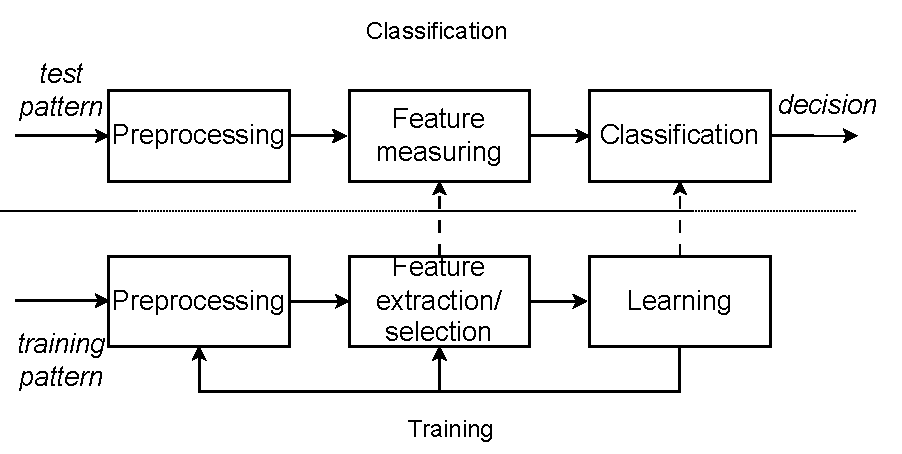
\includegraphics[width=0.7\textwidth]{pattern.pdf}
	\caption{Schemat modelu systemu wykrywającego wzór \cite{Pattern:ResearchGate}}
\end{figure}
\FloatBarrier %zatrzymanie przenoszenia rysunku

Zgodnie z~nią, wykrywanie w~takim systemie (na rys. 2.5 \textit{test pattern}, gdyż w~ten sposób można testować taki system) zaczyna się od \textit{preprocessingu} danych - usuwany jest z~odbieranych informacji szum \cite{medium:pattern}; może to być zarówno szum sygnału dźwiękowego, jak i~np. związany z~zdjęciem. Następnie odbywa się wydobywanie cech kluczowych \textit{feature measurement}, gdzie wydobywane są tylko te istotne, na podstawie których może odbywać się później detekcja. Klasyfikator używa wydobytych wcześniej cech do detekcji na podstawie odpowiedniego algorytmu oraz bazy danych (modelu), która powstała podczas uczenia maszynowego \textit{training}.

Proces uczenia maszynowego wygląda podobnie jak dla \textit{test pattern}. Zaczyna się też od \textit{preprocesingu}, po czym odbywa się ekstrakcja cech - są mierzone cechy charakterystyczne, po czym są wybierane te, które są najistotniejsze dla klasyfikatora - które umożliwiają mu wykonanie najlepszych wykryć. Sprawdzane jest na podstawie zbioru testowego, czy wykrycia pokrywają się z~oczekiwaniami, jeżeli nie, szukane są kolejne cechy i~poprawiany jest model tworzony podczas bezpośredniej procedury uczenia się - tworzenia modelu dla klasyfikatora. Ważne jest, aby zbiór testowy był inny niż zbiór, na podstawie którego model się uczy - po to, aby test był wiarygodny.

Gdy zbiór testowy zawiera też odpowiedzi dla danych próbek - jest to uczenie \textit{nadzorowane} - minimalizuje to liczbę błędów, ale wymaga dużej pracy po stronie projektanta systemu, lub \textit{uczenie nienadzorowane}, gdy tych odpowiedzi nie ma, co powoduje większą liczbę błędów, ale nie potrzebuje dużej ingerencji projektanta systemu \cite{nadzor}.



\subsubsection{Algorytm k-najbliższych elementów}

Obecnie jednym z~najpopularniejszych klasyfikatorów stosowanych jest \textit{sieć neuronowa} \cite{Wiki:neuron}, jednakże wymaga ona bardzo rozbudowanej architektury, aby mogła efektywnie przetwarzać i~rozpoznawać wzorce. W~kontekście potrzeb projektowanych rozwiązań, poszukiwano metody, która wymagałaby mniejszej ilości danych przy równoczesnym zachowaniu skuteczności działania.

Alternatywą dla rozbudowanych sieci neuronowych jest \textbf{algorytm k-najbliższych sąsiadów} (\textit{KNN}), który korzysta z~metod uczenia nadzorowanego. Wizualizację działania tego algorytmu można przedstawić na przykładzie rozkładu danych w~przestrzeni dwuwymiarowej, co ilustruje rysunek 2.6.

\begin{figure}[h]
	\centering
	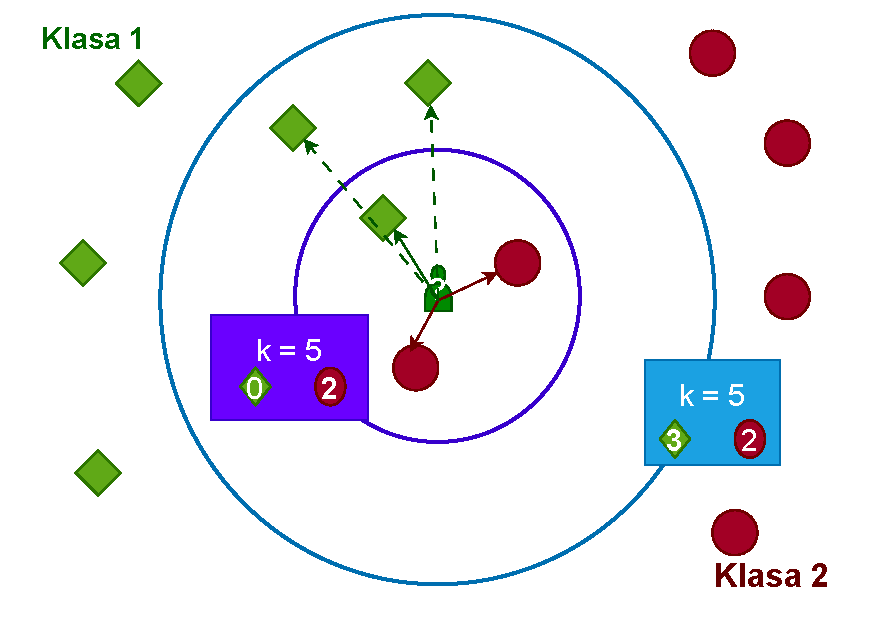
\includegraphics[width=0.5\textwidth]{KNN.pdf}
	\caption{Przykład działania algorytmu \textit{KNN} w~dwuwymiarowej przestrzeni}
\end{figure}
\FloatBarrier %zatrzymanie przenoszenia rysunku

Algorytm \textit{KNN} analizuje rozkład punktów danych, dzieląc je na grupy w~zależności od podanych kryteriów i~przypisując odpowiednie etykiety. Głównym założeniem tego modelu jest przekonanie, że dane bliskie sobie w~przestrzeni cech są podobne do siebie, a~te daleko rozmieszczone są od siebie różne.

Proces działania algorytmu KNN obejmuje kilka kluczowych etapów.
\begin{itemize}
	\item Ustalenie parametru k, czyli liczby najbliższych sąsiadów, która będzie brana pod uwagę.
	\item Obliczenie odległości między testowanym przykładem a~każdym z~przykładów w~zbiorze danych.
	\item Posortowanie odległości od najmniejszej do największej.
	\item Wybranie k najbliższych sąsiadów.
	\item Klasyfikacja na podstawie najczęściej występującej klasy wśród k wybranych sąsiadów.
\end{itemize}

Model KNN oblicza podobieństwo na podstawie odległości między punktami na wykresie. Im większa odległość między punktami, tym mniejsze jest ich podobieństwo. Na przykład, jeśli dla  k=3 prawidłowym wykryciem jest klasa 2, a~dla 
k=5 klasa 1, pokazuje to, jak wybór parametru k może wpływać na wynik klasyfikacji. Metoda \textit{K Najbliższych Sąsiadów z~ważeniem głosów w~zależności od odległości sąsiadów} bierze pod uwagę głosy dotyczące klasyfikowanego wzorca z~wagą zależną od odległości każdego z~najbliższych sąsiadów do tego wzorca \cite{KNN:AGH}.

Szczególnie interesującą odmianą jest \textit{K Najbliższych Sąsiadów z~ważeniem głosów w~zależności od odległości sąsiadów}, gdzie głosy są ważone w~zależności od odległości — im punkt danych jest bliższy testowanemu przykładowi, tym większe ma znaczenie jego głos w~klasyfikacji \cite{KNN:unite}.

\subsection{Urządzenia IoT}

\textbf{Internet rzeczy (IoT)} oznacza sieć obiektów fizycznych — \textit{rzeczy} — które są wyposażone w~czujniki, oprogramowanie i~inne technologie, umożliwiające łączenie się i~wymianę danych z~innymi urządzeniami i~systemami za pośrednictwem Internetu. Urządzenia te obejmują zarówno zwykłe przedmioty gospodarstwa domowego, jak i~zaawansowane narzędzia przemysłowe \cite{Oracle:IoT}.

\subsubsection{Techniki przesyłu danych}

Urządzenia \textit{IoT} zazwyczaj używają interfejsów bezprzewodowych do przesyłania informacji, zarówno pośrednio (przy użyciu bramki), jak i~bezpośrednio. Do najczęściej wykorzystywanych należą: \textbf{WIFI}, \textbf{Bluetooth - BLE}, \textbf{Telefonia komórkowa}, \textbf{LoRa}, \textbf{Sigfox} oraz \textbf{ZigBee} \cite{KomunikacjaIx}.

\subsubsection{Mowa w~IoT}

W ramach tej pracy realizowany jest projekt węzła \textit{IoT} sterowanego mową, ponieważ sterowanie działaniem aplikacji \textit{IoT} za pomocą mowy w~języku naturalnym wydaje się być najbardziej perspektywiczne i~naturalne. Jednak dobre rezultaty mogą być osiągnięte tylko przy użyciu specjalizowanych rozwiązań, takich jak układy scalone. Pozwala to uniknąć konieczności utrzymywania szybkiego połączenia internetowego oraz zapewnia wydajność energetyczną \cite{SpeechI}.

\newpage
\section{Model referencyjny}

\subsection{Wybór danych treningowych dla sztucznej inteligencji}

Sercem systemów rozpoznawania mowy jest sztuczna inteligencja. Aby jej użyć, należało znaleźć dane treningowe, które pozwoliłyby na stworzenie odpowiedniego modelu, umożliwiającego skuteczną detekcję wyrazów. Model musiał zawierać wystarczającą ilość danych, aby mógł wykrywać wyrazy wypowiadane zarówno głosem męskim, jak i~damskim, uwzględniając różne tony głosu oraz zniekształcenia powstałe np. w~wyniku wad wymowy czy szumu w~otoczeniu.

W tym celu użyto zbioru nagrań prostych komend w~języku angielskim (baza \textit{mini\_speech\_commands} dostępna w~zasobach Uniwersytetu Cornell \cite{Baza:Mowa}), zawierającego tysiące nagrań różnych komend o~częstotliwości próbkowania $f_s$ =16~kHz. Jest to częstotliwość pozwalająca na przechowanie wystarczająco dobrej jakości dźwięku, na podstawie którego można wykrywać wyrazy (zgodnie z~twierdzeniem o~próbkowaniu można w~takim przypadku przechowywać dźwięki z~zakresu [0, 8000] Hz, co pozwala na przechowywanie wszystkich dźwięków związanych z~mową - patrz rys. 2.1).

Model zawierał nagrania takich wyrazów, jak w~tabeli 3.1.

\begin{figure}[h]
	\centering
	\begin{tabular}{|r|r|r|}
		\hline
		Wyraz & Ilość nagrań & Liczba sylab\\
		\hline
		Backward & 1 664 & 2\\
		Bed 	 & 2 014 & 1\\
		Bird 	 & 2 064 & 1\\
		Cat 	 & 2 031 & 1\\
		Dog 	 & 2 128 & 1\\
		Down 	 & 3 917 & 1\\
		Eight 	 & 3 787 & 1\\
		... & ... & ...\\
		Wow & 2 123 & 1 \\
		Yes & 4 044 & 1 \\
		Zero & 4 052 & 2\\
		
		\hline
	\end{tabular}
	\caption{Wyrazy zawarte w~bazie \textit{mini\_speech\_commands} \cite{Baza:Mowa}}
\end{figure}
\FloatBarrier %zatrzymanie przenoszenia rysunku

Taki model pozwolił na swobodne wydawanie poleceń urządzeniu słuchającemu podczas testów metody wykrywania wyrazów, o~której mowa w~dalszej części tego rozdziału. Do stworzenia modelu wybrano 16 wyrazów: \textbf{up, down, left, right, yes, stop, sheila, go, on, off, marvin, four, happy, cat, tree, house}. Lista zawiera wyrazy zarówno jedno-, jak i~dwusylabowe.

\subsection{Koncepcja metody wykrywania }

Zanim opracowano koncepcję całego systemu rozpoznawania mowy, należało przemyśleć metodę wykrywania pojedynczych wyrazów, a~następnie stworzyć model testowy, który sprawdziłby pomysł na rozwiązanie problemu. Zgodnie z~założeniami pracy, metoda ta miała być przystosowana do urządzeń o~małych zasobach, przede wszystkim pamięciowych. Inspiracją do stworzenia takiej metody była implementacja rozpoznawania prostych wyrazów przez 16~MHz-owy mikrokontroler \textit{AVR} \cite{SpeechArduino}. Metodę tę jednak rozwinięto, aby zwiększyć odsetek poprawnych wykryć przez system. Zaproponowano więc rozwiązanie zaprezentowane na rys. 3.2.

\begin{figure}[h]
	\centering
	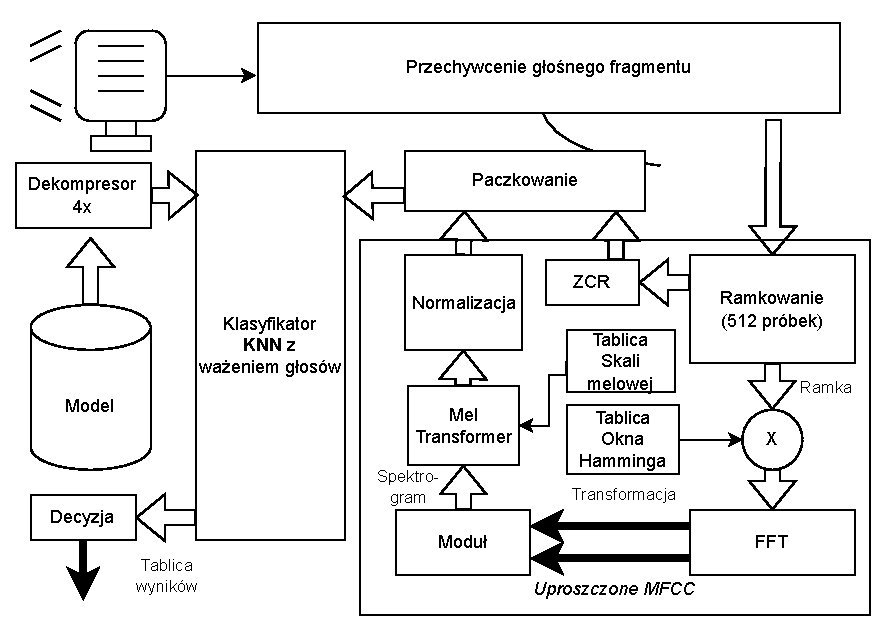
\includegraphics[width=1\textwidth]{Detekcja.pdf}
	\caption{Detekcja wyrazów w~projektowanym systemie}
\end{figure}
\FloatBarrier %zatrzymanie przenoszenia rysunku

Najpierw przechwytywany jest głośny fragment z~sygnału mikrofonowego. Następnie uzyskane nagranie przetwarzane jest przez \textit{uproszczone} \textit{MFCC} (wyliczenie spektrogramu w~skali melowej wraz z~\textit{ZCR} \textit{Zero Crossing Rate}) \cite{Wiki:ZCR}. Otrzymany w~ten sposób profil dźwięku jest przetwarzany przez wariant \textit{Klasyfikatora KNN z~ważeniem głosów} na podstawie modelu dekompresowanego przy użyciu autorskiego algorytmu. Klasyfikator ten wydaje ostateczną decyzję.

Metodę tę zaimplementowano w~środowisku \textit{Python} (wersja 3.11 uruchamiana przez \textit{PyCharm} IDE), tworząc model referencyjny, co umożliwiło wykonanie wstępnych testów, dopasowanie długości ramek oraz przetestowanie metod realizacji poszczególnych procedur (np. zamiana dziedziny ze skali liniowej na melową), aby uzyskać jak najlepszy odsetek prawidłowych wykryć. Pomogło to w~szybszej realizacji powyższego algorytmu w~sprzęcie.




\subsubsection{Zbieranie próbek}

Pierwszym etapem wykrywania wyrazów jest wybranie głośnego fragmentu z~sygnału mikrofonowego. Urywek ten, z~dużym prawdopodobieństwem, zawiera wyraz, który warto przeanalizować. Fragmenter przechwytuje jedynie nagranie o~długości 1,5 s (precyzja 16-bitowa), ponieważ więcej danych nie zmieściłoby się w~pamięci typowego mikrokontrolera używanego w~urządzeniach \textit{IoT}. Procedurę wyboru tego bloku dźwiękowego ilustruje rys. 3.3.

\begin{figure}[h]
	\centering
	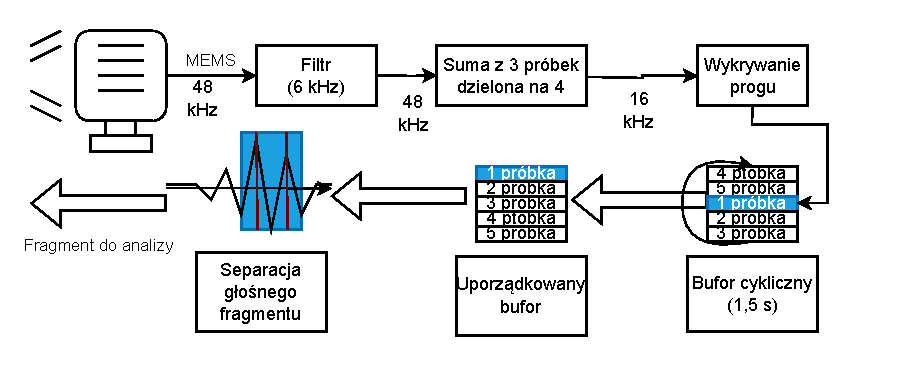
\includegraphics[width=1\textwidth]{Seperated.pdf}
	\caption{Algorytm wyboru fragmentu do analizy z~sygnału mikrofonowego}
\end{figure}

Najpierw przechwytywany jest sygnał bezpośrednio z~mikrofonu o~standardowej częstotliwości 48 kHz. Aby nie przetwarzać niepotrzebnie zbyt dużego pasma oraz przystosować fragment do przetwarzania przez opracowany model (omówiony w~podrozdziale 3.3), należało obniżyć częstotliwość próbkowania do 16 kHz. W~pierwszym etapie fragment przechodzi przez filtr dolnoprzepustowy \textit{FIR} o~częstotliwości granicznej $f_g$ = 6 kHz.

Następnie dokonuje się właściwego obniżenia częstotliwości, tworząc pewnego rodzaju cyfrowy kondensator. Sumowane są 3 próbki, które kolejno trafiły do tego bloku z~filtru, a~następnie dzieli się tę sumę przez 4 (co można zrealizować przesunięciem bitowym o~2). W~ten sposób, nie tracąc zbyt wielu niuansów (które mogłyby zostać utracone, gdyby przepuszczano co trzecią próbkę), obniżono próbkowanie 3-krotnie — z~48~kHz do 16~kHz, co jest zgodne z~modelem.

Następnym krokiem jest zapisywanie powstałych w~ten sposób próbek przez tzw. \textit{bufor cykliczny (kołowy)} \cite{Wiki:Circular}. Pozwala on na odkładanie zdefiniowanej ilości danych (1,5 sekundy nagrania, czyli dla próbkowania 16 kHz będzie to 24000 próbek) bez potrzeby ich ciągłego sortowania, co zmniejsza zużycie zasobów obliczeniowych. Moduł ten czeka, aż przechwyci fragment, którego wartość bezwzględna jest większa od ustalonego progu (ustalany w~zależności od użytego mikrofonu). Następnie bufor przechwytuje jeszcze 0,75~s (12000 próbek), po czym przestaje odbierać sygnał dźwiękowy i~zaczyna sortować bufor. Dzięki temu uzyskuje się uporządkowany przechwycony fragment. W~ten sposób moduł przechwytuje sąsiedztwo głośnej próbki, aby uchwycić możliwie cały wyraz.

Uporządkowany bufor jest normalizowany (normalizacja liniowa do wartości w~zakresie 0 - 512), a~następnie ponownie analizowany pod kątem wydzielenia wyrazu z~nagrania, stosując bardziej ścisłe wymagania. Pozwala to na wychwycenie słowa bez niepotrzebnych fragmentów z~posortowanego bufora. Do tego celu stosuje się algorytm opisany na rys. 3.4.

\begin{figure}[h]
	\centering
	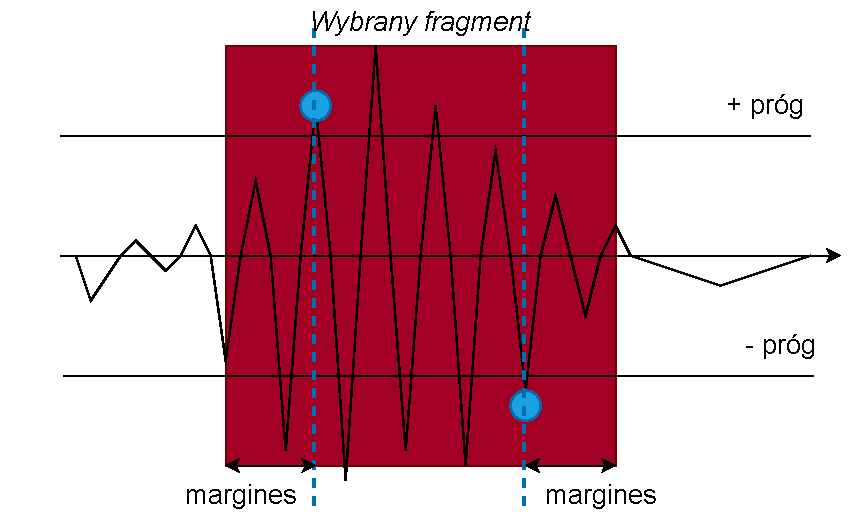
\includegraphics[width=0.7\textwidth]{Select.pdf}
	\caption{Wybór „głośnego” fragmentu do analizy}
\end{figure}
\FloatBarrier %zatrzymanie przenoszenia rysunku

Moduł analizuje kolejno próbki, aż wykryje próbkę o~wartości bezwzględnej równej 128, określonej jako próg. Następnie ustala się, że początek wykrytego fragmentu znajduje się w~próbce o~numerze mniejszym o~długość \textbf{marginesu} (\textit{margin} określony jako 5120 próbek) od analizowanej próbki. Jeżeli numer ten byłby ujemny, ustala się, że początek znajduje się w~zerowej próbce. Następnie analizowane są kolejne próbki, aż ich wartość bezwzględna spadnie poniżej określonego progu. Wówczas odlicza się kolejne próbki niespełniające tego warunku. Jeżeli wykryto próbkę spełniającą warunek, licznik jest zerowany.

Gdy licznik osiągnie wartość marginesu, ustala się koniec fragmentu w~tej próbce. Następnie sprawdzana jest długość fragmentu — czy jest ona odpowiednia (empirycznie określono, że długość takiego fragmentu powinna wynosić od 11000 do 18000 próbek). Jeżeli fragment spełnia ten wymóg, jest on przekazywany do analizy, jeżeli nie, analiza trwa dalej. Jeśli nie został wykryty fragment spełniający warunki, algorytm wraca do przechwytywania próbek przez bufor cykliczny.



\subsubsection{Przetwarzanie sygnałów}


Następnie odbywa się proces przetwarzania sygnałów nazwany roboczo \textit{uproszczonym MFCC}. Metoda ta wykonuje wszystkie kroki określone w~rozdziale 2.2 poza obliczeniem samego cepstrum. Zamiast jego liczenia, używa się \textit{ZCR}, który dodawany jest do każdej ramki spektrogramu \textit{melowego}, co upraszcza metodę, zachowując akceptowalną precyzję.

Najpierw fragment jest ramkowany, tworząc fragmenty o~długości 512 próbek. Uznano (na podstawie testów różnych wariantów wielkości ramki), że jest to wystarczająca precyzja na potrzeby prostej detekcji dźwięków i~ograniczonego słownika. Po podziale ramka przechodzi przez okno \textit{Hamminga}. Próbka ramki jest mnożona przez element tablicy skali melowej o~numerze odpowiadającym próbce (obliczonej wcześniej i~zapisanej w~programie). Następnie obliczana jest szybka \textit{transformacja Fouriera} algorytmem \textit{Cooleya-Tukeya} \cite{CT:FFT}, a~następnie spektrogram — licząc energię każdej próbki widma poprzez obliczenie modułu liczby zespolonej. Zgodnie z~twierdzeniem o~próbkowaniu, należy pobrać jedynie połowę wartości obliczonego spektrogramu, aby uniknąć zapisywania powtarzających się informacji (256 próbek widma).

Następnie dokonuje się zamiany dziedziny ze skali liniowej na skalę melową (logarytmiczną). Ustala się tablicę \textit{mel\_table}, gdzie dla każdej próbki widma w~dziedzinie liniowej określono jej pozycję w~skali melowej. Do tego celu wykorzystano środowisko \textit{Python}, które umożliwiło wygenerowanie tablicy przedstawionej na rys. 3.5.

\begin{figure}[h]
	\centering
	
	\begin{tabular}{|r|r|r|r|r|r|r|r|r|r|r|r|r|r|r|r|r|r|r|r|r|r|r|r|r|r|r|r|}
		\hline
		n		   & 0 & 1 & 2 & 3 & 4 & 5 & 6 & 7 & 8 & ...  & 252 & 253 & 254 & 255 \\
		\hline
		mel\_table[n]& 0 & 4 & 8 & 12 & 16 & 20 & 23 & 27 & 30 & ...    & 252   &   253 &   253 &   253 \\
		\hline
	\end{tabular}
	
	\caption{Tablica skali melowej}
\end{figure}

\FloatBarrier %zatrzymanie przenoszenia rysunku

Tablica ta została użyta w~algorytmie zamiany zaprezentowanym na rys. 3.6.

\begin{figure}[h]
	\begin{lstlisting}[language=Python]
		
		mem = 0
		mel_spect = []
		
		for n in range(256):
			amount = mel_table[n]
			
			if mel_table[n] > mem:
				mem = spect[n]
				
			if mel_table[n] != 0:
				
				for k in range(mel_table[n]):
					mel_spect.append(mem)
				mem = 0
		
	\end{lstlisting}
	\caption{Fragment skryptu wykonanego w~języku \textit{Python} pozwalający na zamianę skali z~liniowej na melową (logarytmiczną)}
\end{figure}
\FloatBarrier %zatrzymanie przenoszenia rysunku

Wraz z~pobraniem wartości tablicy \textit{mel\_table}, spektrogram albo multiplikuje próbkę, albo zbiera ich odpowiednią ilość zgodnie z~powyższym algorytmem. Gdy skończy się zbiór próbek odpowiadających jednej próbce w~skali logarytmicznej, wysyłana jest największa wartość próbki z~tego zbioru. Metoda ta pozwala na prostą implementację w~sprzęcie.

Dla każdej ramki 512 próbek tworzona jest linijka profilu o~długości 320 próbek (256 dla spektrogramu i~64 dla liczby przejść przez zero \textit{ZCR} — bajty o~tej samej wartości). Ustalono, że dla danej ramki maksymalna liczba przejść przez zero wyniesie 255; pozostałe wartości były ignorowane. Fragment taki jest skalowany w~dziedzinie czasu, aby dopasować go do znormalizowanego modelu (do długości 64 pojedynczych linijek profilu stosując interpolację metodą \textit{najbliższego sąsiada} \cite{Skalowanie}). Zabieg ten pozwala na to, aby wolniejsze lub szybsze niż w~modelu wypowiedzenie danego słowa nie wpływało na precyzję detekcji wyrazu.

Spektrogram taki jest normalizowany „logarytmicznie” — tak aby zamienić poziomy mocy danych dźwięków ze skali liniowej na decybelową — stosowaną po to, aby zmieścić dużą rozpiętość ciśnienia akustycznego dźwięków słyszanych przez ludzkie ucho \cite{Sound} w~małej liczbie bitów. Określenie „logarytmicznie” ujęto w~cudzysłowie, gdyż dla uproszczenia przyszłej implementacji sprzętowej tej operacji zastosowano pierwiastek, który pozwala, podobnie jak logarytm, umieścić wspomniane poziomy. Po normalizacji wartości związanych z~widmem, aby zignorować szum w~części związanej ze spektrogramem, usuwa się wartości widma poniżej 16.

Uzyskany w~ten sposób profil na przykładzie nagrania wyrazu \textit{sheila} wygląda tak jak na rys. 3.7.

\begin{figure}[h]
	\centering
	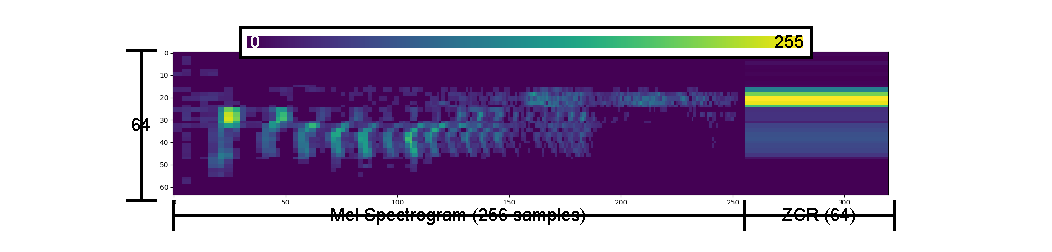
\includegraphics[width=1\textwidth]{Profile.pdf}
	\caption{Profil wyrazu \textit{sheila}}
\end{figure}
\FloatBarrier %zatrzymanie przenoszenia rysunku

Procedura ta umożliwia porównanie go z~innymi profilami uzyskanymi wcześniej, nawet w~innych warunkach.

\subsubsection{Kompresja danych}

Pamięć masowa jest zazwyczaj wąskim gardłem podczas operowania na dużych zbiorach informacji, do których zalicza się model sztucznej inteligencji. Dane te muszą być ładowane bezpośrednio z~nośnika podczas szukania najlepszego dopasowania przez klasyfikator. Systemy embedded, w~tym IoT, mają zbyt mało pamięci operacyjnej, aby przechować tam cały model. Ponieważ taki proces jest wolniejszy niż przetwarzanie danych bezpośrednio z~pamięci \textit{RAM}, należało opracować sposób, który rekompensowałby wolniejsze czytanie zawartości pamięci. Jednym z~takich rozwiązań jest kompresja danych.

Aby uprościć ten proces, zdecydowano się na autorski algorytm \textit{stratny} \cite{Wiki:kompresja}, dostosowany do przetwarzania wartości nieujemnych, skupiony głównie na przechowywaniu maksimów. Rysunek 3.8 ilustruje jego działanie.

\begin{figure}[h]
	\centering
	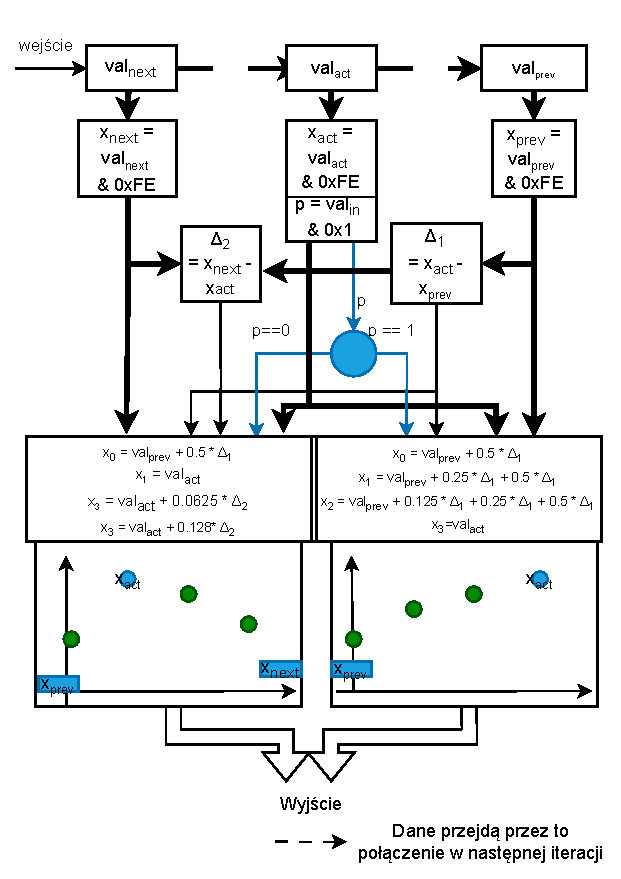
\includegraphics[width=0.8\textwidth]{Kompresja.pdf}
	\caption{Ilustracja dekompresji danych}
\end{figure}

\FloatBarrier %zatrzymanie przenoszenia rysunku

Algorytm przechowywał trzy wartości: próbkę poprzednią ($val_{prev}$), aktualna ($val_{act}$) oraz próbka następna ($val_{next}$). Każda z~tych wartości zawierała informację o~pozycji maksimum z~precyzją do dwóch próbek (najmłodszy bit) oraz pozostałe bity związane z~właściwą wartością maksimum. Wartości tych parametrów można uzyskać, odpowiednio maskując wartość, jak na rys. 3.8.

Na potrzeby dalszego przetwarzania wyliczane były różnice między aktualną próbką a~poprzednią ($\Delta_1$) oraz pomiędzy następną a~aktualną ($\Delta_2$). W~zależności od tego, jaką pozycję w~nowo powstałej czwórce miała wartość aktualna  ($p$), przewidywano się dwa scenariusze.
\begin{itemize}
	\item \textbf{p = 1}, wówczas do obliczeń potrzebne są jedynie wartość aktualna i~poprzednia. Do wartości poprzedniej dla kolejnych próbek dodaje się coraz większą część $\Delta_1$, aż w~ostatniej próbce podaje się wartość aktualną (patrz schemat powyżej).
	\item \textbf{p = 0}, wówczas do obliczeń używa się wszystkich wartości obliczonych w~kroku poprzednim. Najpierw do wartości poprzedniej próbki dodaje się połowę  Następnie dodaje się w~następnych wartościach do wartości aktualne kolejne większe części $\Delta_2$.
\end{itemize}

Uzyskane w~ten sposób próbki są przekazywane dalej jako wyjściowy strumień danych. Algorytm dostosowano tak, aby zamiast niepotrzebnych mnożeń można było zastosować przesunięcia bitowe, co redukuje potrzebę zastosowania bloków DSP w~FPGA.

Algorytm ten, podobnie jak poprzedni, nadaje się do implementacji w~sprzęcie, gdyż pozwala na zastosowanie \textit{potokowania} \cite{Potokowanie}. Metoda ta umożliwia załadowanie do klasyfikatora cztery razy większej ilości danych w~tej samej jednostce czasu, ponieważ obliczenia są zazwyczaj znacznie szybsze od ładowania danych z~nośnika.

\subsubsection{Algorytm KNN z~ważeniem głosów}

Po opracowaniu metod ładowania danych i~pomiaru cech kluczowych danego fragmentu dźwięku, należało opracować prototyp klasyfikatora przystosowanego do rozpoznawania słów z~modelu. Na potrzeby tej analizy zastosowano algorytm z~uwzględnieniem ważenia głosów.

Zdecydowano się jednak na nietypowy wariant tego algorytmu. Obliczane były na bieżąco różnice między profilem dźwięku otrzymanym po pomiarze cech kluczowych a~profilami pochodzącymi z~modelu. Od każdej próbki profilu uzyskanego podczas analizy sygnału dźwiękowego z~mikrofonu odejmuje się odpowiadającą jej próbkę z~danego profilu modelu. Wszystkie te różnice są sumowane, aby dla każdego profilu z~modelu uzyskać własną sumę różnic, która jest odległością dla algorytmu \textit{KNN}. W~ten sposób klasyfikator analizuje cały model.

Wybiera się najmniejsze osiem takich odległości, po czym są one sortowane. Następnie przydziela się im punkty: kolejno najmniejszej odległości 8, drugiej 7 itd., po czym sumuje się punkty dla sum różnic, które należały do tej samej kategorii w~modelu (do tego samego słowa). Słowo o~największej liczbie punktów klasyfikator uznaje za właściwe wykrycie. Aby uniknąć możliwych omyłkowych wykryć w~sytuacji, gdy detekcja jest niejednoznaczna, minimalna liczba punktów dla poprawnego wykrycia wyrazu wynosi 15. Algorytm ten opisano na rys. 3.9.

\begin{figure}[h]
	\centering
	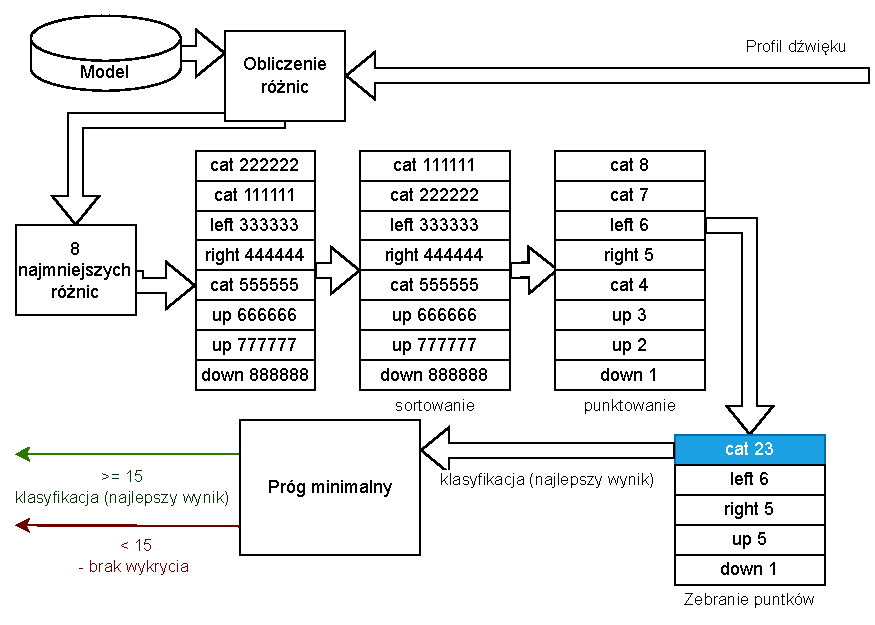
\includegraphics[width=1\textwidth]{Klasyfikator.pdf}
	\caption{Schemat działania klasyfikatora}
\end{figure}

\FloatBarrier %zatrzymanie przenoszenia rysunku
\subsection{Trening modelu oraz ocena metody detekcji}


Aby to wykonać, przeanalizowano pierwsze 256 nagrań słów wybranych do stworzenia słownika wyrazów wykrywanych przez węzeł. Fragmenty te miały już próbkowanie wynoszące 
$f_s$ = 16~kHz, więc nie istniała potrzeba obniżania próbkowania. Nie było również potrzeby wyboru głośnego fragmentu przy użyciu bufora cyklicznego, gdyż trening odbywał się na urządzeniu o~znacznie większej mocy obliczeniowej niż urządzenie docelowe.

Dla każdego nagrania w~zestawie treningowym dla modelu dokonywano \textit{ekstrakcji cech}, która jest bardzo podobna do pomiaru cech kluczowych (charakterystyczne dla algorytmu \textit{KNN}), jak pokazano na ilustracji 3.10.

Finalnie przetworzone nagrania wyrazów były kompresowane, aby zmniejszyć ich rozmiar czterokrotnie zgodnie z~algorytmem określonym w~rozdziale 3.2.3. Tak powstałe profile wyrazów zapisywano jako pliki binarne - każdy dla pojedynczego nagrania. Skompresowany model składający się z~16 wyrazów ważył 20 MB (po 5 kB na skompresowany profil). Dzięki temu możliwe było pełne przetestowanie modelu referencyjnego metody detekcji wyrazów. Testy empiryczne w~środowisku \textit{Python} pozwoliły dopasować parametry, uzyskując satysfakcjonujący odsetek prawidłowych wykryć podczas wydawania poleceń komputerowi.

\begin{figure}[h]
	\centering
	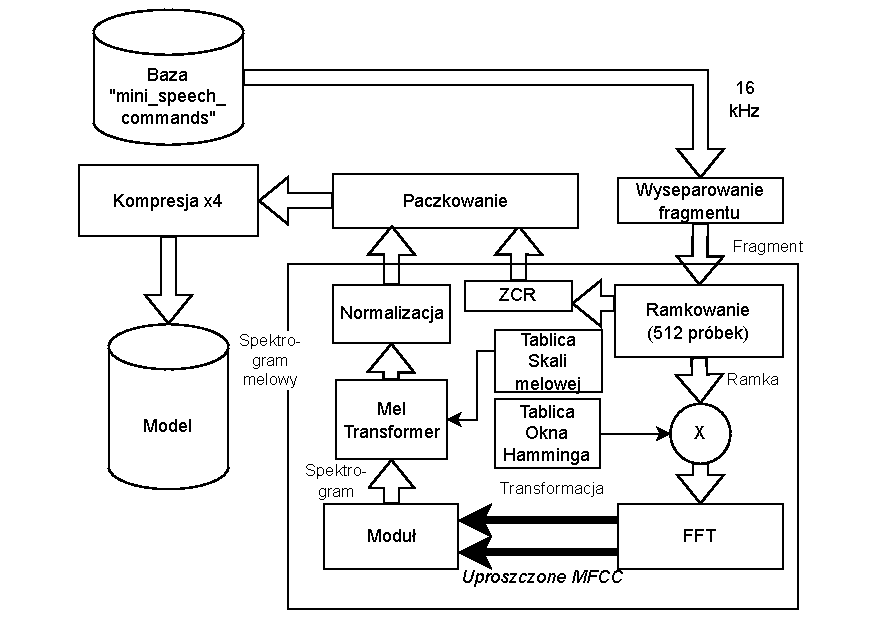
\includegraphics[width=1\textwidth]{Uczenie.pdf}
	\caption{Schemat treningu modelu sztucznej inteligencji dla projektowanego systemu}
\end{figure}
\FloatBarrier %zatrzymanie przenoszenia rysunku

\subsubsection{Wnioski z~testów}

Pewne wyrazy są lepiej wykrywane niż inne (dla niektórych odsetek poprawnych detekcji wynosił nawet 98\%, podczas gdy dla najgorzej wykrywanych 72\%). Niemniej jednak, projektowane urządzenie powinno być przystosowane do wykrywania jedynie kilku rozkazów, w~zależności od kontekstu, w~którym ma zostać użyte. Można więc pozostawić projektantom systemu dobór zestawu wyrazów (metodą prób i~błędów), aby były wykrywane te, które są interesujące. W~systemach sztucznej inteligencji istotne jest również wykrywanie wyrazów spoza puli, więc odrzucone wyrazy mogą posłużyć do wychwytywania takich dźwięków.

Najdłużej trwającą procedurą jest przeszukiwanie modelu przez klasyfikator. Analiza w~środowisku \textit{Python} dla 8 wyrazów trwa około 9 sekund, podczas gdy pozostałe operacje (np. pomiar cech kluczowych) zajmują zaledwie 100 - 250 ms. Operacja porównania w~sztucznej inteligencji wymaga więc akceleracji sprzętowej, podobnie jak przetwarzanie sygnałów podczas pomiaru cech kluczowych oraz normalizacja. Operacje te wykonują dużo obliczeń na liczbach zmiennoprzecinkowych i~pozwalają na łatwe zwielokrotnienie podczas \textit{przetwarzania potokowego}.

Poprawność wykryć na poziomie około 90\% oznacza, że 1 wyraz na kilkadziesiąt był wykrywany błędnie. Użytkownik rozwiązania musiał mieć możliwość ponownej próby podania rozkazu, aby poprawić błędne wykrycie. Minimalizowało to ryzyko wysyłania błędnych informacji do serwera zarządzającego większym systemem.

Zdecydowano się na zastosowanie \textbf{prostego systemu dialogowego}, umożliwiającego weryfikację poprawności wykryć. Najpierw użytkownik mówił do węzła jego hasło wywoławcze (wybrano imię żeńskie znajdujące się w~bazie, czyli \textit{Sheila}). Po wykryciu węzeł odpowiadał głosowo „\textit{Yes}”, po czym użytkownik miał 5 sekund na podanie hasła, które zostanie przesłane dalej do przetworzenia. Gdy system wychwycił hasło, oznajmiał, co wykrył, mówiąc „\textit{You said ...}”, gdzie w~miejsce trzech kropek wstawiano wykryty wyraz. W~przypadku braku wykrycia system mówił „\textit{Could you repeat}”. Użytkownik, słysząc błędne wykrycie, mógł anulować komendę, wymawiając ją ponownie, po czym węzeł ponownie mówił, co wykrył, uprzedzając to słowem „\textit{Sorry}”. Użytkownik miał 3 próby; jeśli przez 3 próby nie udało się poprawnie wykryć wyrazu lub urządzenie nie wychwyciło żadnej komendy przez czas oczekiwania, uznawano, że nie można wykryć wyrazu. Urządzenie wtedy mówiło „\textit{I can't understand you. Sorry}” i~wracało do stanu nasłuchu rozkazów. Jeśli przekroczono czas, ale nie anulowano wykrycia, węzeł wysyłał rozkaz dalej po interfejsie bezprzewodowym.

Należało więc w~węźle opracować prosty system audio, aby mógł wypowiadać wyrazy. W~celu uproszczenia rozwiązania nie zastosowano syntezy mowy, lecz wygenerowane wcześniej nagrania. Do tego celu wykorzystano narzędzie online \cite{Nagrania}, gdzie wygenerowano dźwięki wyrazów na potrzeby wspomnianego systemu.

Urządzenie, w~którym zaimplementowano metody z~modelu referencyjnego, musiało również sprawdzać sprawność swoich komponentów, takich jak nośnik danych czy mikrofon. Uznano również, że warto sprawdzać, czy w~pobliżu urządzenia znajduje się użytkownik. Najprostszym rozwiązaniem tego problemu było zastosowanie czujnika odległości, co pozwalało dodatkowo sprawdzić, czy głośny dźwięk nie jest przypadkowym dźwiękiem z~tła. Podczas testów niejednokrotnie wykrywano słowo, mimo że nikt go nie wymawiał ani nie był w~pobliżu komputera.


\subsection{Podobne rozwiązania}

Podczas opracowywania pracy, nie znaleziono węzła IoT, który w~układach FPGA wykorzystywałby algorytm k-najbliższych sąsiadów oraz ładował bezpośrednio dane z~nośnika. Koncepcja podobna do tego projektu została opisana w~artykule \cite{KWS} dotyczącym rozpoznawania wyrazów przez małe modele w~najnowszych platformach \textit{ARM Cortex-M7} (\textit{DS-CNN KWS}). W~ramach tej technologii używano sprzętowo zoptymalizowanych sieci neuronowych, wykorzystujących minimalną ilość zasobów, a~także wspomagano operacje przetwarzania sygnałów.

Modele te zostały stworzone przy użyciu różnych metod optymalizacji, takich jak \textit{przycinanie sieci} i~\textit{kwantyzacja parametrów}, aby stworzyć warianty \textit{CNN} (\textit{Convolutional Neural Network} \cite{CNN}), które są w~stanie zapewnić wyniki prawie tak dokładne jak pełne \textit{CNN}.

We wnioskach do projektu autorzy (firma \textit{ARM}) twierdzą, że wspomniane wyżej rozwiązanie jest w~stanie skutecznie wykrywać wyrazy z~małego słownika wraz z~pomiarem cech kluczowych (stosując pełne \textit{MFCC}) w~ciągu 12 ms, przy użyciu około 70 kB pamięci. Daje to wydajność zbliżającą się do 10 wykryć na sekundę z~wykorzystaniem zasobów pamięciowych osiągalnych dla urządzeń typowo stosowanych w~\textit{IoT}. Parametry te posłużyły do oceny tworzonego rozwiązania podczas testów sprzętowych.

Wyżej wspomniane rozwiązanie ma podobne założenia do tworzonego w~ramach tej pracy — pomiar cech kluczowych dźwięku i~przetwarzanie ich w~ramach modelu sztucznej inteligencji bez użycia przetwarzania chmurowego w~rozsądnym czasie i~z użyciem małej ilości zasobów obliczeniowych oraz przy zastosowaniu akceleracji sprzętowej.

Istnieje także inne podobne rozwiązanie w~pełni wykonane z~użyciem układu \textit{FPGA}, bez wykorzystania procesora \cite{FPGA:DIGIKEY}. Inną propozycją jest rozwiązanie na układzie firmy \textit{Intel} \cite{Intel:Recogn}, które wykorzystuje \textit{HPS} — wbudowany w~układ \textit{FPGA} procesor \textit{ARM}, w~którym używa się systemu operacyjnego Linux.


\subsection{Przygotowanie nośników danych}

Aby węzeł mógł ładować dużą ilość danych, jak na klasę urządzenia wykonywaną w~tym projekcie, zdecydowano się na zastosowanie kart \textit{SD} \cite{karta::SD} do przechowywania nagrań i~modelu. Umożliwiały one proste nagrywanie zawartości z~poziomu komputera. Aby uprościć procedurę odczytu danych, zrezygnowano z~zastosowania systemu \textit{FAT-32} \cite{FAT32} i~zastosowano własny system plików. W~pierwszym sektorze karty znajdował się wykaz plików (nagrań i~modeli) oraz informacja o~autorze obrazu (rys. 3.11).

\begin{figure}[h]
	\centering
	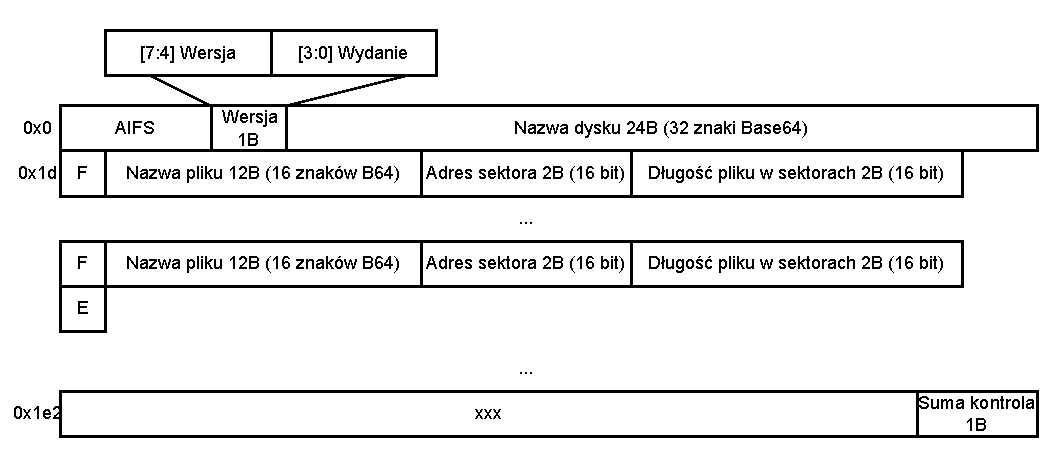
\includegraphics[width=0.8\textwidth]{PlikiAIFS.pdf}
	\caption{Schemat ułożenia danych w~pierwszym sektorze nośnika}
\end{figure}
\FloatBarrier %zatrzymanie przenoszenia rysunku

Znajdują się tutaj informacje o~systemie plików (nagłówek \textit{AIFS}) oraz jego wersja, dzięki czemu urządzenie może sprawdzać kompatybilność z~własnym oprogramowaniem zawartości pamięci zewnętrznej. Następnie znajdujemy zakodowane informacje za pomocą wariantu kodowania \textit{Base64} \cite{Base64}. W~dalszej części sektora znajduje się lista plików; każdy plik rozpoczynał się bajtem 0x46 ('F' w~tablicy ASCII), a~listę kończył bajt 0x45 ('E' w~tablicy ASCII). Każdy plik ma odnośniki do adresów sektorów oraz informację o~długości pliku. Plik zawsze składa się z~pewnej liczby sektorów będących jeden po drugim w~pamięci. Podczas konceptualizacji systemu założono niezmienność danych, stąd zrezygnowano z~zabiegów ułatwiających dopisywanie nowych plików lub zmianę ich zawartości. Ostatnim znakiem sektora jest suma kontrolna, będąca najmłodszymi 8 bitami sumy jedynek binarnych w~sektorze.

Tutaj zapisano odnośniki do 48-kHzowych nagrań 16-bitowego dźwięku na potrzeby systemu dialogowego oraz wskazania do nagłówka modelu.

Schemat nagłówka modelu znajduje się na rys. 3.12.

\begin{figure}[h]
	\centering
	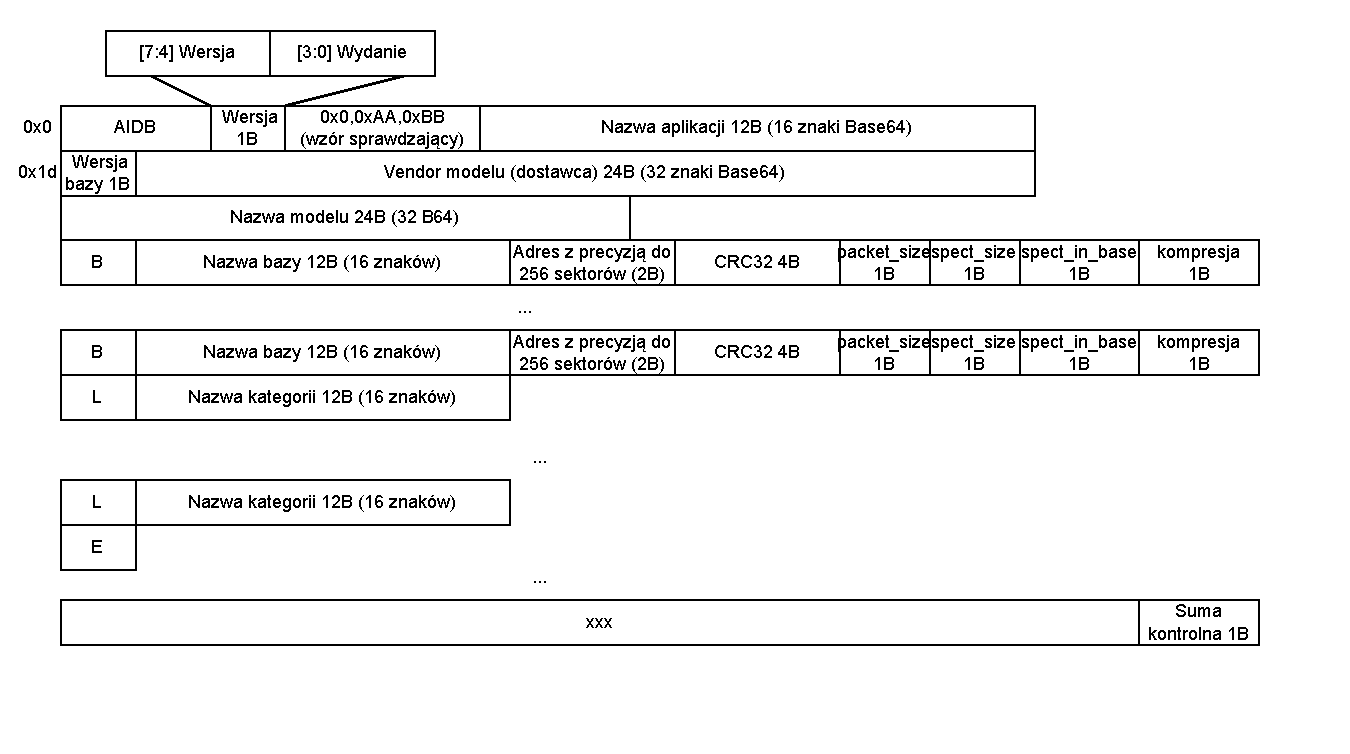
\includegraphics[width=0.95\textwidth]{PlikiAIDB.pdf}
	\caption{Schemat nagłówka modelu}
\end{figure}
\FloatBarrier %zatrzymanie przenoszenia rysunku

Na początku nagłówka znajdują się informacje o~wersji standardu bazy oraz dane na jej temat (dostawca, nazwa bazy). Następnie znajduje się lista zastosowanych baz w~modelu wraz z~kluczowymi parametrami - pozycja w~pamięci, suma kontrolna danej bazy dla przetwarzania wielu nośników na raz. Jeżeli system przetwarza wiele pamięci zewnętrznych na raz, wówczas pozycja zarówno nagłówka modelu, jak i~samych baz, musi być na każdym nośniku taka sama. Podobnie identyczne są parametry konfiguracyjne bazy (\textit{packet\_size} - liczba profili dla danej kategorii w~bazie, \textit{spect\_size} - rozmiar skompresowanego profilu w~bajtach, \textit{spect\_in\_base} - liczba kategorii w~bazie oraz kompresja 1 dla czterokrotnej i~0 dla dwukrotnej) oraz nazwy kategorii.

Nagłówek ten weryfikuje się podobnie jak pierwszy sektor za pomocą sumy kontrolnej. Zbiór tych informacji nie powinien być większy niż 1 sektor. Pozycje baz danych mogą się znajdować w~sektorach o~adresach będących wielokrotnością 256. Aby uzyskać prawdziwy adres sektora, wartość pola adresu dla danej bazy należy pomnożyć przez 256. Wynika to z~ograniczeń komponentu klasyfikatora zastosowanego w~systemie. Profile w~modelu są ułożone po kolei zgodnie z~parametrami nagłówka. Kategorie są przydzielane po kolei według kolejności baz danych na liście. Z~perspektywy klasyfikatora kategoria jest jedynie numerem, więc gdy są 2 bazy po 8 kategorii, wówczas pierwsza baza na liście otrzyma pierwsze 8, a~druga baza pozostałe.

Do zapisu liczb stosuje się notację \textit{little endian}. Zawartość nośnika generowano za pomocą jednego ze skryptów modelu referencyjnego, dzięki czemu tworzono plik .bin z~obrazem karty. Kartę tę nagrywano przy użyciu programu \textit{HxD} \cite{HxD}.

System projektowano pod kątem zastosowania sektorów o~rozmiarze 512 bajtów, co jest standardową wartością dla większości pamięci Flash, MMC czy kart SD \cite{karty:SD}\cite{karty:EMMC}. Stosowanie innych rozmiarów nie było obsługiwane w~projekcie.

Model podzielono najpierw na 2 bazy po 8 kategorii. Następnie uzyskane dane rozdzielono pomiędzy 4 karty pod kątem potencjalnego przetwarzania wielu nośników jednocześnie. Na każdym nośniku było 64 profile dźwięku dla każdej kategorii. Bazy otrzymały parametry: \textit{packet\_size} = 64, \textit{spect\_size} = 5, \textit{spect\_in\_base} = 8 i~z zastosowaniem kompresji czterokrotnej, aby zmieścić większą ilość profili na mniejszym obszarze nośnika.

\newpage
\section{Implementacja sprzętowej detekcji wyrazów}

\subsection{Platforma docelowa}

System został zrealizowany na płycie \textit{Terrasic DE10-Lite} zawierającej układ \textit{FPGA Intel MAX 10} - model \textit{10M50DAF484C7G} \cite{Intel:MAX}. Układ ten umożliwia uruchomienie na nim procesora \textit{Nios IIe} wraz z~układami wspomagającymi opisanymi w~języku \textit{HDL}. W~tym projekcie użyto języka \textit{Verilog} HDL. Pozwala on na użycie wbudowanego w~niego komponentu \textit{ADC} oraz wbudowanej pamięci flash \textit{UFM} (\textit{User Flash Memory} \cite{IntelUFM}), którą można zaprogramować z~poziomu logiki programowalnej. Jest to cecha nietypowa dla układów \textit{FPGA}, pozwalająca na umieszczenie całego systemu cyfrowego w~jednym chipie wraz z~oprogramowaniem - procesor potrafił bootować się z~tej pamięci.

Układ ten ma wystarczająco dużo zasobów (bloków logicznych), aby pomieścić procesor soft-core, koprocesory wspomagające sztuczną inteligencję, przetwarzanie sygnałów oraz sterowanie dołączonymi do niego komponentami zewnętrznymi, używającymi standardowych elektronicznych interfejsów (np. \textit{SPI} czy \textit{I$^2$C}). Na tle innych układów \textit{FPGA} jest energooszczędny \cite{Intel:MAX}, nie wymaga aktywnego chłodzenia, co czyni go idealnym do systemów racjonalnych pod względem kosztów i~uzyskanego efektu (\textit{cost-sensitive applications}). Dzięki temu jest dobrą platformą do prototypowania procesora głównego węzła \textit{Internetu Rzeczy} z~potrzebą akceleracji sprzętowej pewnych zadań wykonywanych przez takie urządzenie.

\begin{figure}[h]
	\centering
	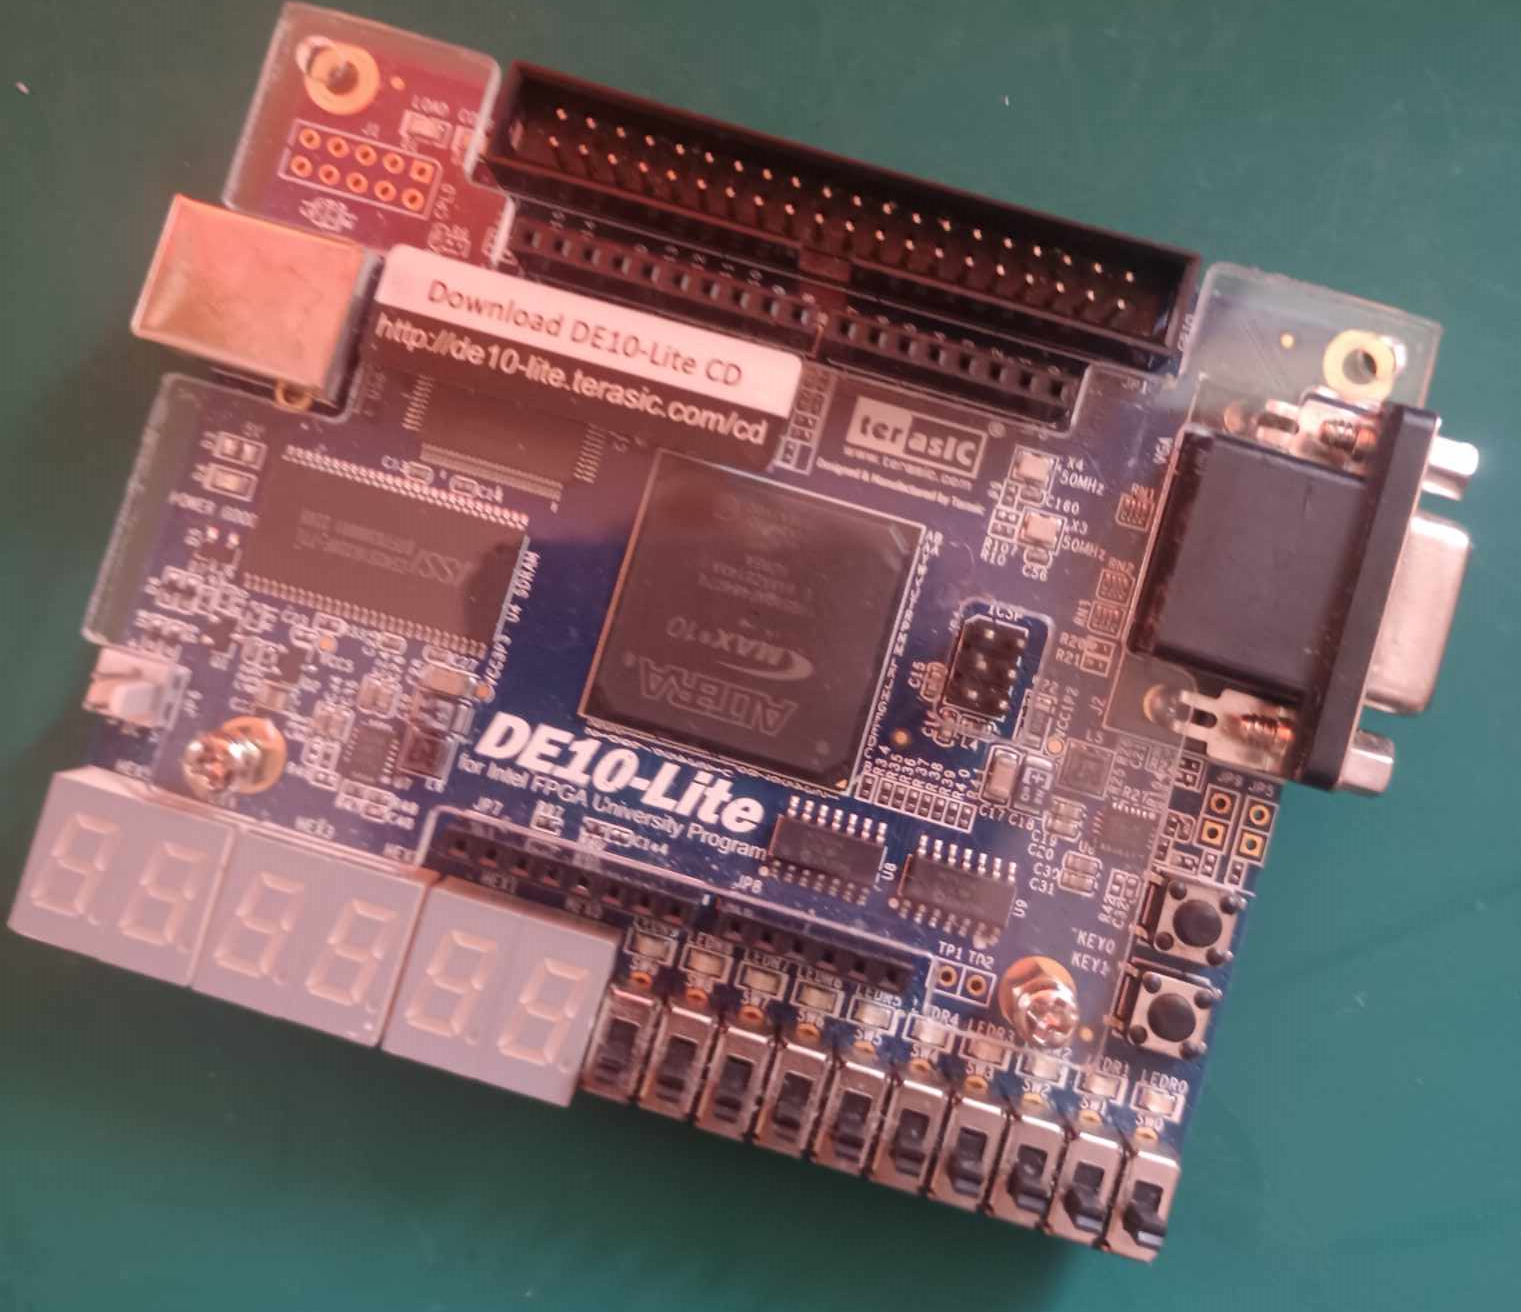
\includegraphics[width=0.5\textwidth]{de10-lite.png}
	\caption{Płytka \textit{Terrasic DE10-Lite}}
\end{figure}
\FloatBarrier %zatrzymanie przenoszenia rysunku

Projekt procesora głównego opracowano w~środowisku współpracującym z~układami \textit{Intel MAX} - \textit{Quartus Prime Lite Edition} w~wersji \textit{18.1}.

\subsection{Zarys architektury rozwiązania}

Projektowanie systemu rozpoczęto od opracowania w~sprzęcie układów pozwalających na wykonanie wymagających obliczeniowo operacji (obliczanie profilu, normalizacja wartości oraz klasyfikacja). Procesor działa na zegarze 100 MHz, nie wspiera sprzętowo mnożenia, dzielenia oraz operacji na liczbach zmiennoprzecinkowych. Taka specyfikacja CPU nie jest wystarczająca, aby efektywnie wykonywać wyżej wymienione operacje. Dodatkowo, rozmiar pamięci \textit{RAM} dostępnej jako \textit{BRAM} w~układzie \textit{FPGA} nie pozwala na buforowanie modelu w~niej (jej rozmiar wynosi 196 kB, co jest o~rząd wielkości mniejsze niż nawet skompresowany model). Aby ograniczyć zużycie prądu przez układ, nie używa pamięci zewnętrznej \textit{RAM} i~bezpośrednio ładuje model z~nośnika zewnętrznego.

Opracowano więc system detekcyjny, który ilustruje rys. 4.2.

\begin{figure}[h]
	\centering
	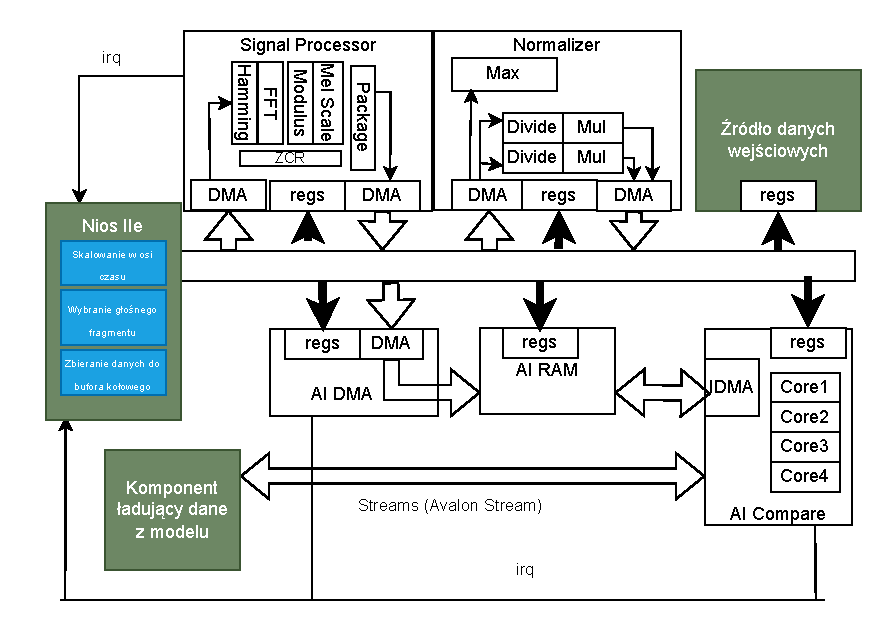
\includegraphics[width=1\textwidth]{detect_system_FPGA.pdf}
	\caption{Uproszczony schemat systemu wykrywającego}
\end{figure}
\FloatBarrier %zatrzymanie przenoszenia rysunku

System sprzętowo akceleruje trzy operacje: działanie klasyfikatora przez komponent \textit{AI\_compare}, normalizację danych (zarówno logarytmiczną, jak i~liniową) w~\textit{Normalizer}, oraz przetwarzanie sygnałów w~\textit{Signal\_Processor} do wyznaczania profilu wychwyconego dźwięku. Pozostałe zadania, takie jak przechwycenie głośnego fragmentu, skalowanie w~dziedzinie czasu oraz nasłuchiwanie danych z~komponentu \textit{I/O}, wykonuje procesor \textit{Nios}. Operacje dopasowania spektrogramu w~czasie oraz ramkowania nie są akcelerowane sprzętowo, aby uprościć rozwiązanie. Zadania te wykonywane są przez CPU na tyle szybko, że nie wpływa to na komfort użytkowania rozwiązania.

Procesor sygnałowy (\textit{Signal\_Processor}) wykonuje operacje nadania okna \textit{Hamminga}, transformację \textit{FFT}, wylicza moduł z~transformacji, aby uzyskać spektrogram, po czym zamienia go do skali melowej i~łączy go z~\textit{ZCR}. Moduł pobiera przez \textit{DMA} jedną ramkę, po czym zapisuje przez drugie \textit{DMA}.

Podobne przetwarzanie wykorzystuje \textbf{Normalizer}, odpowiadający za normalizację wartości z~pamięci. Działa on w~dwóch trybach: liniowym i~logarytmicznym. Dla uproszczenia budowy komponentu, zamiast obliczania logarytmów, oblicza pierwiastek kwadratowy, tak jak w~modelu referencyjnym. Ten tryb obsługuje \textit{linijki profilu}; tylko pierwsze \textit{n} (parametr określony w~rejestrze konfiguracyjnym) próbek w~linijce jest normalizowane logarytmicznie.

Dane po przygotowaniu pełnego profilu są ładowane do oddzielnej pamięci. W~systemie znajduje się instancja \textbf{AI\_RAM}, aby komponent klasyfikatora miał do niej szybszy dostęp. Aby ładować dane szybciej, zastosowano specjalny komponent \textbf{AI\_DMA}. Pozwala on na szybkie przekopiowanie i~obróbkę danych, które będą dalej porównywane przez klasyfikator. Dzięki niemu dodatkowo są usuwane wartości zbyt małe (aby pozbyć się szumu) oraz nadawane wagi dla danych części linijki profilu, mnożąc w~odpowiedni sposób wartości. Dla tego projektu wagi są takie same i~wynoszą jeden - funkcjonalność ta została wprowadzona przyszłościowo, na potrzeby tworzenia uniwersalnej platformy \textit{IoT} dla sztucznej inteligencji, zgodnie z~celami tej pracy.

Ostatnim komponentem akcelerującym obliczenia jest klasyfikator \textit{KNN} - \textbf{AI\_compare}. Komponent ten pobiera dane z~nośnika pośrednio przez układ obsługujący nośnik zewnętrzny danych. Aby przyspieszyć proces, układ używa czterech takich nośników. Pozwala to na szybsze wykonywanie klasyfikacji modelu. W~sprzęcie mogą one działać jednocześnie bez uszczerbku na wydajności. Dane z~nośników są porównywane z~danymi w~pamięci \textit{AI\_RAM}, po czym wyniki klasyfikacji są udostępniane na rejestry.

Komponenty informują procesor o~zakończeniu operacji przez przerwania. Konfiguracja ich odbywa się przez ustawienie odpowiednich wartości rejestrów. Do komunikacji pomiędzy procesorem a~komponentami wykorzystuje się interfejs \textit{Avalon Memory Mapped} \cite{Intel:AVMM} (dla \textit{DMA} jest w~trybie \textit{master}, zaś dla rejestrów - \textit{regs} - w~wersji \textit{slave}).

Moduły zostały opracowane w~języku opisu sprzętu \textit{Verilog HDL}. W~celu stworzenia systemu z~CPU, do którego będą podłączone wspomniane komponenty, zastosowano narzędzie dołączone do środowiska \textit{Quartus Prime}, przede wszystkim \textit{Platform Designer} \cite{PDes}.

\subsection{Direct Access Memory}

Komponentem powszechnie używanym w~tym projekcie jest uproszczone \textbf{DMA} (\textit{Direct Access Memory}). Korzystają z~niego komponenty \textit{AI\_DMA}, \textit{Normalizer} i~\textit{Signal\_Processor}. Moduł pozwala na zapisanie lub odczytanie jednocześnie 32-bitowej wartości z~danego adresu przestrzeni adresowej. Do tego celu wykorzystano \textit{FSM} komunikujący się z~szyną danych procesora interfejsu \textit{Avalon Memory Mapped} w~trybie \textit{master}. Automat stanów \textit{DMA} opisano na rys. 4.3.

Moduł komunikuje się z~resztą komponentu, w~którym się znajduje, za pomocą własnego interfejsu: do podkomponentu trafiają dane na temat adresu (przez sygnał \textit{dma\_addr} o~szerokości 32 bitów, zgodnie z~architekturą systemu), to, czy dane mogą być odczytane, czy zapisane (przez sygnał \textit{dma\_read} lub \textit{dma\_write}) oraz dane do zapisu przez \textit{dma\_writedata} (o szerokości 32 bitów, zgodnie z~rozmiarem słowa procesora). Moduł powinien zwracać sygnał \textit{dma\_rdy} w~przypadku zakończenia operacji i~ewentualnie \textit{dma\_readdata} o~szerokości 32 bitów z~odczytanymi danymi.

\begin{figure}[h]
	\centering
	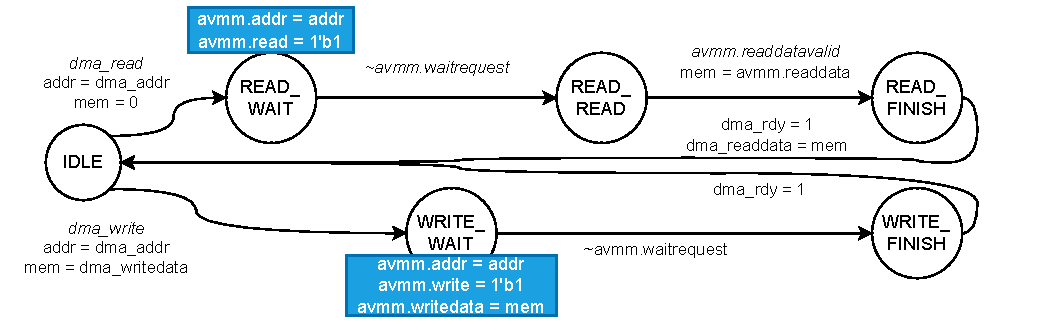
\includegraphics[width=1\textwidth]{DMA_FSM.pdf}
	\caption{Automat stanów modułu \textit{DMA}}
\end{figure}
\FloatBarrier %zatrzymanie przenoszenia rysunku

\subsection{Komponent DSP \textit{Signal\_processor}}
\subsubsection{Architektura komponentu}

Procesor sygnałowy realizuje przetwarzanie potokowe na potrzeby analizy odebranych danych dźwiękowych. Rysunek 4.4 prezentuje uproszczoną architekturę rozwiązania.

Komponent poprzez moduł \textit{DMA} pobiera dane z~pamięci, które trafiają do modułu \textit{loader}. Na podstawie parametrów \textit{start\_addr} i~\textit{init} ustawianych przez procesor, pobierana jest z~pamięci ramka danych. Następnie przekazuje się ją do podkomponentu realizującego okno \textit{Hamminga} (\textit{hamming\_window}) interfejsem strumieniowym \textit{Avalon Stream}. Dalej realizowane jest przetwarzanie potokowe.

\begin{figure}[h]
	\centering
	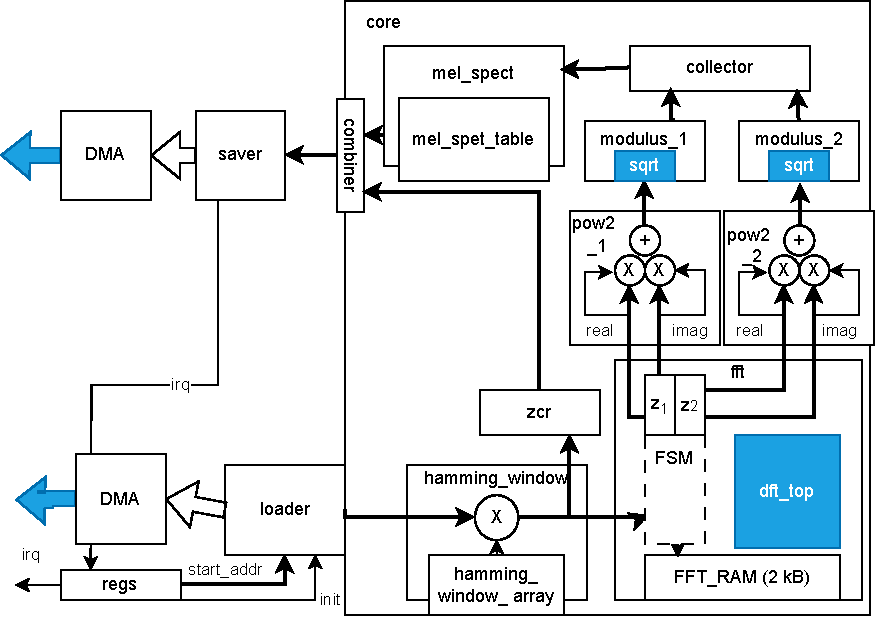
\includegraphics[width=1\textwidth]{SignalProcessor.pdf}
	\caption{Architektura koprocesora sygnałowego}
\end{figure}
\FloatBarrier %zatrzymanie przenoszenia rysunku

Dane poprzez interfejs strumieniowy trafiają równocześnie do komponentu realizującego \textit{FFT} (\textit{fft}) oraz do podmodułu liczącego przejścia przez zero (\textit{zcr}). Transformator zwraca dwie wartości zespolone (składające się z~części rzeczywistej \textit{real} i~urojonej \textit{imag}). Dane w~tej postaci ponownie przekazywane są strumieniowo dalej do komponentów obliczających sumę kwadratów, a~następnie do podmodułów liczących pierwiastki z~tych liczb (w ten sposób oblicza się moduł liczby zespolonej). Następnie \textit{collector} zbiera dane z~dwóch strumieni liczących moduły, układając je w~prawidłowej kolejności i~przekazuje je do modułu \textit{mel\_spect}.

Po zamianie ze skali liniowej na melową, moduł \textit{saver} przekazuje dane do modułu \textit{combiner} wraz z~danymi z~\textit{zcr}. Tam tworzona jest linijka profilu z~uzyskanych informacji, po czym trafia ona do modułu \textit{saver}. Zapisuje on dane pod odpowiednio ustawionym przez parametry adresem (\textit{start\_addr\_write}), a~następnie po zakończeniu wysyła informację do podmodułu z~rejestrami o~wysłaniu przerwania.

Komponent przetwarza w~trakcie jednej operacji (inicjowanej za pomocą nadania odpowiednich wartości rejestrom konfiguracyjnym) jedną ramkę składającą się z~512 próbek 16-bitowych. Efektem tego jest otrzymanie profilu składającego się z~320 próbek. Komponent nie pozwala na modyfikację rozmiaru ramki poprzez zmianę wartości rejestru.

Do przekazywania danych między modułami realizującymi operacje potokowe wykorzystuje się interfejs \textit{Avalon Stream} z~użyciem sygnałów \textit{data} (16 bitów), \textit{valid} i~\textit{ready}. Wszystkie podmoduły wracają do stanu pierwotnego po otrzymaniu sygnału \textit{init}, poza komponentem z~rejestrami konfiguracyjnymi.


\subsubsection{Ładowanie danych do rdzenia i~zapisywanie}

Za ładowanie danych do rdzenia i~zapis uzyskanych po obliczeniach wyników odpowiadają moduły \textbf{saver} i~\textbf{loader}. Są one automatami stanów, które sterują podmodułami \textit{DMA} i~odpowiednio zapisują do pamięci dane uzyskane z~interfejsu strumieniowego \textit{Avalon Stream}, oraz pobierają wartości przez \textit{DMA} i~przekazują je do rdzenia obliczeniowego. Schematy wyżej wspomnianych automatów znajdują się na rysunkach 4.5 i~4.6.

\begin{figure}[h]
	\centering
	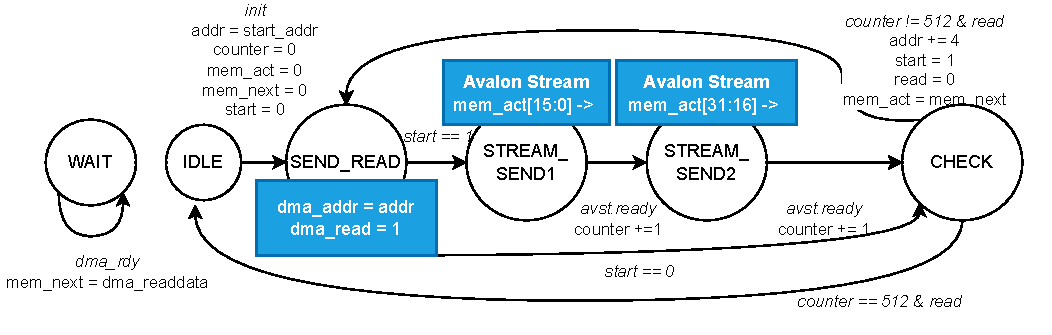
\includegraphics[width=0.8\textwidth]{reader_signal_FSM.pdf}
	\caption{Automat stanów modułu \textit{loader}}
\end{figure}
\FloatBarrier %zatrzymanie przenoszenia rysunku

Automat \textbf{loader} ładuje dane z~przestrzeni adresowej i~przekazuje je na interfejs strumieniowy \textit{Avalon Stream}. Automat po inicjacji ładuje 512 próbek 16-bitowych z~adresu wskazanego przez parametr \textit{start\_addr}, po czym wraca do stanu \textit{IDLE}. Jedno słowo zawiera dwie próbki, dlatego po dokonaniu jednej transakcji \textit{DMA} moduł wysyła strumieniowo oddzielnie dwie wartości. Komponent pozwala na odbieranie danych z~\textit{DMA} i~wystawianie ich na interfejsie strumieniowym w~tym samym czasie, zrównoleglając te operacje.

\begin{figure}[h]
	\centering
	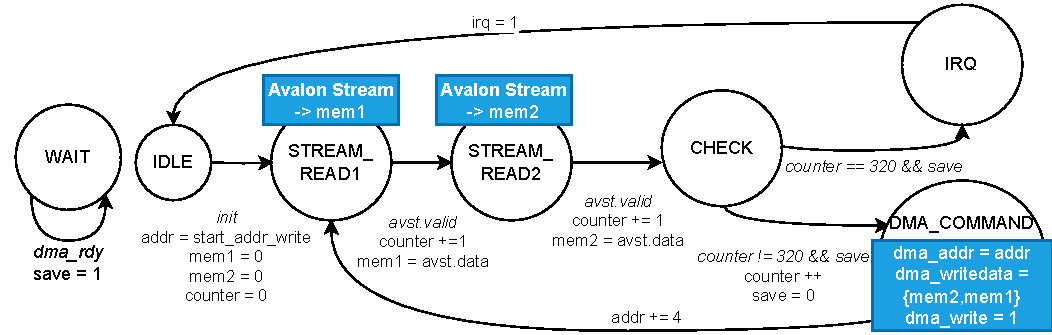
\includegraphics[width=0.8\textwidth]{saver_signal_FSM.pdf}
	\caption{Automat stanów modułu \textit{saver}}
\end{figure}
\FloatBarrier %zatrzymanie przenoszenia rysunku

Podobnie zrównoleglony jest moduł \textbf{saver}. Może on w~tym samym czasie odczytywać dane z~interfejsu \textit{Avalon Stream} oraz czekać na odpowiedź od \textit{DMA} o~zakończeniu zapisywania danych. Po odczytaniu dwóch wartości moduł składa z~nich słowo (tak jak na rys. 4.6 w~stanie \textit{DMA\_COMMAND}), po czym przekazuje je do \textit{DMA}, aby je zapisać. Moduł zapisuje 320 próbek 16-bitowych pod adresem określonym w~parametrze \textit{start\_addr\_write}. Gdy wspomniana ilość danych zostanie wysłana, moduł wysyła sygnał \textit{irq}, aby moduł zewnętrzny mógł później przekazać przerwanie do procesora o~zakończeniu pracy całego komponentu.


\subsubsection{Moduł okna Hamminga}
Jednym z~etapów przetwarzania sygnałów pod kątem pomiaru cech kluczowych, wspomnianym w~rozdziale 3.2.2, jest przetworzenie ramki przez okno \textit{Hamminga}. W~tym celu stworzono moduł \textbf{hamming\_window}.

Moduł ten jest prostym automatem stanów. Najpierw w~stanie \textit{IDLE} czeka na dane w~interfejsie \textit{Avalon Stream} od modułu \textit{loader}. Odebrana liczba jest rozbijana na wartość bezwzględną (poprzez negację bitową i~dodanie jedynki w~przypadku wykrycia liczby ujemnej) oraz na jej znak. Następnie moduł przechodzi do stanów \textit{LOAD\_DATA\_1} i~\textit{LOAD\_DATA\_2}. Stany te służą do odczytu danych po interfejsie natywnym z~pamięci \textit{hamming\_window\_array} z~wartościami współczynników okna \textit{Hamminga}. Dla każdej odebranej wartości przydzielana jest zgodna z~kolejnością odbioru wartość z~tablicy w~wcześniej wspomnianej pamięci \textit{ROM}.

Następnie, w~stanie \textit{MUL}, uzyskaną wartość z~pamięci mnoży się z~odebraną po interfejsie strumieniowym. Do tego celu wykorzystuje się bloki \textit{DSP}. Następnie, w~stanach \textit{SEND\_FFT} i~\textit{SEND\_ZCR}, wynik operacji jest wystawiany na interfejsach strumieniowych odpowiednio do modułów \textbf{fft} i~\textbf{zcr}. Finalnie moduł wraca do stanu \textit{IDLE}.

Wynik przed jego wystawieniem na interfejs jest przekształcany na podstawie wcześniej ustalonego znaku; najpierw wybiera się bity w~zakresie [31:16] do przekazania, gdyż podczas obliczeń wykorzystuje się algebrę stałoprzecinkową (\textit{fixed point}). Wartości w~pamięci \textit{ROM} są 16-bitowe i~mają 16 bitów po przecinku (współczynniki nie mogą być ujemne, więc ignoruje się pierwszą liczbę przed przecinkiem). Wartość otrzymywana po interfejsie strumieniowym jest również 2-bajtowa, ale nie ma żadnych miejsc po przecinku. Następnie, zgodnie z~notacją uzupełnień do dwóch, gdy wartość otrzymana na wejściu jest ujemna, podobnie jak podczas odbioru wartości na wejściu, wartość jest negowana i~dodawana do niej jedynka.

\subsubsection{Moduł ZCR}

Moduł liczący przejścia przez zero \textbf{zcr} jest prostym automatem stanów. Przechowuje on dwie próbki: poprzednią w~rejestrze \textit{lmem} oraz aktualną w~rejestrze \textit{mem}, rozpoczynając analizę po otrzymaniu obu wartości. Po odebraniu danych w~stanie \textit{IDLE} z~podmodułu \textit{hamming\_window}, moduł przechodzi do stanu \textit{CHECK}.

W stanie \textit{CHECK} sprawdzany jest znak bieżącej i~ostatniej wartości (najstarszy bit liczby - gdy jest on ustawiony na 1, liczba jest ujemna). Uzyskane w~ten sposób sygnały są poddawane operacji \textit{XOR}. Gdy na tym bicie uzyskano stan wysoki, inkrementuje się licznik. Jeśli wartość wynosi 255 lub jest jej równa, nie wykonuje się wspomnianej operacji. Po otrzymaniu 512 wartości, na podstawie kolejnego licznika liczącego odebrane dane, moduł przechodzi do stanu \textit{RETURN}, po czym wystawia na interfejsie strumieniowym do podmodułu \textit{combiner} obliczoną liczbę przejść przez zero, a~następnie wraca do stanu \textit{IDLE}.

\subsubsection{Moduł FFT}

Mając na względzie złożoność takiego komponentu, do realizacji transformacji Fouriera wykorzystuje się zewnętrzną implementację \cite{Spiral}. Aby zmieścić cały system w~ograniczonych zasobach, szczególnie pamięciowych, stosuje się iteracyjną, a~nie strumieniową wersję komponentu wykonującego 512-punktową transformację. Szybkość wykonywanej operacji, mimo zastosowania wolniejszej iteracyjnej wersji, jest znacznie wyższa niż potencjalne wykonywanie tej operacji na procesorze \textit{Nios} (zgodnie z~rozdziałem 7.1.2). Zaplanowano, aby w~przyszłości stworzyć własną wersję tego komponentu, co poprawi wydajność rozwiązania.

Aby podłączyć ten moduł do komponentów korzystających z~interfejsów strumieniowych \textit{Avalon Stream}, stworzono \textit{wrapper} dla zewnętrznego komponentu o~nazwie \textbf{fft}. Podmoduł ten składa się z~automatu stanów, wspomnianego wcześniej modułu oraz pamięci (2 kB) komunikującej się za pomocą natywnego interfejsu. Automat stanów najpierw odbiera dane i~zbiera je w~pamięci. Następnie, zgodnie ze specyfikacją \cite{Spiral}, do modułu \textit{dft\_top} ładowane są próbki z~pamięci (dwie wartości zespolone na raz - jedna wartość zespolona zawsze wynosi zero). Transakcję rozpoczyna się sygnałem \textit{next}, po czym strumieniowo ładuje się dane do modułu. Komponent przystosowano do liczenia transformacji dla 32-bitowych wartości, co poprawia dokładność obliczeń w~notacji \textit{fixed\_point}. Podczas projektowania modułu zastosowano precyzję z~12 bitami po przecinku. Aby to uzyskać, przesuwa się pobrane z~interfejsu wartości o~12 bitów. Dla ujemnych liczb, 4 najmłodsze bity zamienia się na \textit{0xF}, a~najstarsze 12 bitów na \textit{0xFFF}.

\begin{figure}[h]
	\centering
	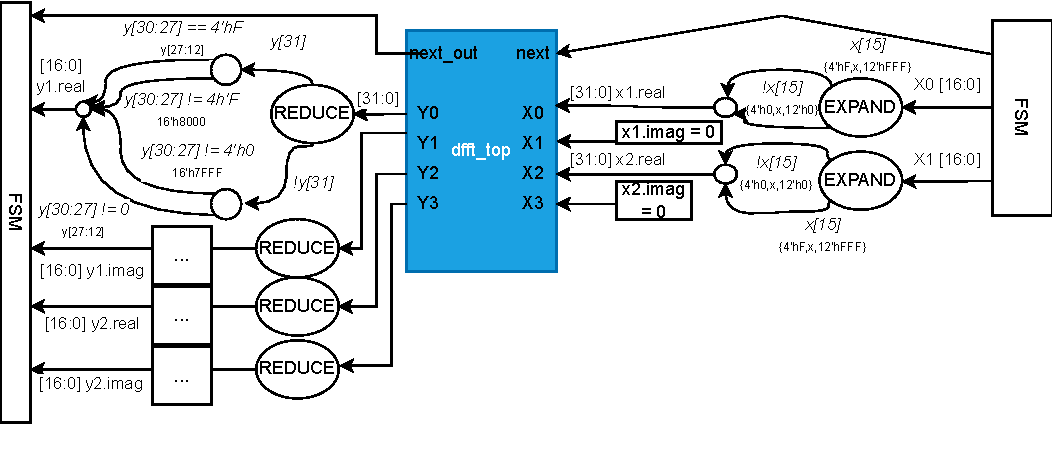
\includegraphics[width=0.9\textwidth]{FSM_conv.pdf}
	\caption{Zamiana wartości 16-bitowych na 32-bitowe oraz schemat wejść i~wyjść do zewnętrznego modułu \textit{dfft\_top}}
\end{figure}
\FloatBarrier %zatrzymanie przenoszenia rysunku

Następnie, po otrzymaniu sygnału \textit{next\_out}, pierwsze 256 wyników z~wyjścia modułu są zapisywane, z~wyłączeniem pierwszych trzech próbek, które są wpisywane jako zera. Redukuje to wpływ piku FFT dla zerowej częstotliwości. Aby zachować odpowiednią notację, moduł pobiera tylko przedział bitowy [27:12]. Gdy uzyskany wynik nie mieści się w~wspomnianym zakresie, dla liczby ujemnej zapisuje się odpowiednio maksymalną wartość ujemną, a~dla dodatnich - maksymalną wartość dodatnią dla 16-bitowej liczby. Finalnie komponent wystawia wyniki na dwa interfejsy strumieniowe: na \textit{transform\_1} dla parzystych numerów próbek i~na \textit{transform\_2} dla nieparzystych. Interfejsy te różnią się od standardowego \textit{Avalon Stream} tym, że przesyłają one dwie wartości - zespoloną 16-bitową część \textit{real} i~urojoną \textit{imag} przy jednej transakcji.

Komponent ten nie jest dobrze zrównoleglony, niemniej jego małe zapotrzebowanie na bloki logiczne w~układzie pozwala na łatwe wdrożenie tego rozwiązania w~prototypie, bez czasochłonnych modyfikacji.


\subsubsection{Moduły obliczania modułu z~wartości zespolonej}

Moduły \textbf{pow2} i~\textbf{modulus} odpowiadają za obliczanie wartości bezwzględnej (modułu) z~liczby zespolonej. \textbf{Pow2} odpowiada za obliczanie sumy kwadratów z~wykorzystaniem bloków \textit{DSP}.

W stanie \textit{IDLE} moduł otrzymuje po interfejsie strumieniowym 16-bitową wartość zespoloną (sygnał \textit{real}) i~urojoną (sygnał \textit{imag}) od \textit{fft}, po czym przechodzi do stanu \textit{ABS}, gdzie uzyskuje wartość bezwzględną podobnie jak w~module \textit{hamming\_window} (rozdział 4.3.3). Znak liczby jest ignorowany, gdyż kwadrat wartości rzeczywistej jest zawsze nieujemny. Następnie, w~stanie \textit{MUL}, liczby są mnożone przez siebie, a~potem w~stanie \textit{SUM} sumowane. Finalnie uzyskany wynik 32-bitowy jest wystawiany na interfejsie \textit{Avalon Stream} do komponentu \textbf{modulus}.

Moduł \textbf{modulus} oblicza pierwiastek kwadratowy odebranej liczby, po czym przekazuje wynik do bloku \textit{collector} (tak jak na schemacie 4.4). Do tego celu wykorzystuje zewnętrzną implementację komponentu obliczającego zgodnie z~artykułem \cite{Root}. Dodano własny wrapper, który umożliwia obsługę interfejsu strumieniowego przez wspomnianą implementację. Uzyskana wartość ma 16 bitów.

Wyniki z~dwóch modułów \textit{modulus} zbiera \textit{collector}, łącząc je i~przekazując jednym interfejsem do \textit{mel\_spect}. Najpierw odbierana jest liczba z~modułu \textit{modulus\_1}, potem wystawiana na zbiorczym interfejsie, a~następnie z~\textit{modulus\_2}.

\subsubsection{Moduł zamiany z~skali liniowej na logarytmiczną}

Moduł \textit{mel\_scale} odpowiada za zamianę dziedziny z~liniowej na logarytmiczną zgodnie ze skalą melową. Do tego celu wykorzystano algorytm opracowany podczas projektowania modelu referencyjnego w~sekcji 3.2.3. Stworzono automat stanów realizujący ten algorytm, którego schemat znajduje się na rysunku 4.8.

Komponent w~stanie \textit{IDLE} czeka na dane na wejściu strumieniowym, po czym sprawdza, czy odebrana wartość nie jest większa od wcześniej ustalonego maksimum. Jeśli tak jest, zawartość rejestru jest nadpisywana. Następnie moduł odbiera z~tablicy \textbf{mel\_spect\_table} liczby oznaczające pozycję danej wartości w~skali melowej - dla aktualnej i~następnej próbki. Liczby te ustalane są zgodnie z~licznikiem liczącym ilość transakcji wejściowych. Podczas syntezy pamięć stała została znacznie uproszczona do postaci kilku bloków logicznych. Następnie jest liczona różnica, która oznacza, ile razy dana próbka ma być upraszczana. Gdy ta różnica jest większa od zera, moduł przechodzi do stanu \textit{RETURN}, gdzie wystawiana na wyjściowy interfejs \textit{Avalon Stream} wartość maksymalna jest zapisywana tyle razy, ile wyniosła różnica, a~w~innym przypadku moduł wraca do stanu \textit{IDLE}.

\begin{figure}[h]
	\centering
	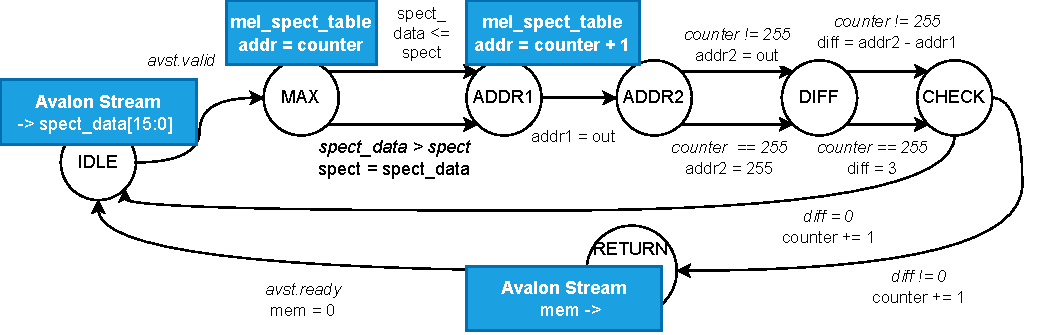
\includegraphics[width=0.8\textwidth]{mel_spect_signal_FSM.pdf}
	\caption{Automat stanów modułu \textit{mel\_spect}}
\end{figure}
\FloatBarrier %zatrzymanie przenoszenia rysunku

Dane wystawione trafiają do modułu \textbf{combiner}, gdzie są łączone z~wartościami obliczonymi w~module \textit{zcr}. Najpierw przekazuje się 256 próbek spektrogramu melowego poprzez interfejs strumieniowy do bloku \textit{saver}. Następnie moduł odbiera wartość z~licznika przejść przez zero, po czym wystawia tę liczbę 64 razy - tak aby uzyskać linijkę profilu o~długości 320.
 
\subsubsection{Rejestry sterujące komponentem}

Wewnętrznie komponent \textit{Signal\_Processor} jest sterowany przez procesor za pomocą rejestrów udostępnianych przy użyciu modułu \textbf{parameters}. Umożliwia on zapisywanie wartości do rejestrów oraz wystawianie przerwania, które jest zwalniane po nadpisaniu odpowiednich rejestrów. Do manipulacji wspomnianym modułem z~poziomu CPU wykorzystuje się interfejs \textit{Avalon Memory Mapped}. Moduł używa uproszczonej wersji rejestrowej bez sygnałów \textit{wait\_request} itp. Wykaz adresów pamięci wraz z~funkcjami przedstawiono na rysunku 4.9.

\begin{figure}[h]
	\centering
	\begin{tabular}{|r|r|r|}
		\hline
		Adres & Funkcja & Zakresy wartości\\
		\hline
		0x0 & Zwolnienie przerwania & Nadpisanie jakąkolwiek wartością \\
			&						& tego adresu powoduje wyzerowanie\\
			&						& przerwania procesorowego\\
		
		\hline 
		0x4 & Adres odczytu spektrogramu & [31:0]\\
		\hline
	\end{tabular}
\end{figure}
\begin{figure}[h]
	\centering
	\begin{tabular}{|r|r|r|}
		\hline
		Adres & Funkcja & Zakresy wartości\\
		\hline 
		0x8 & Adres zwrotu profilu & [31:0]\\
		
		\hline 
		0xc & Inicjacja operacji &Nadpisanie jakąkolwiek wartością \\
		&& tego adresu powoduje  \\
		&& rozpoczęcie generowania profilu\\
		\hline
	\end{tabular}
	
	\caption{Rejestry komponentu \textit{Signal\_Processor}}
\end{figure}
\FloatBarrier %zatrzymanie przenoszenia rysunku

Wszystkie wspomniane rejestry są w~trybie tylko do zapisu. Offset komponentu wynosi 0x30000, zaś numer przerwania 5. Komponent podłączony jest do szyny procesora, łącząc jego oba DMA z~pamięcią główną \textit{RAM}. Zachowuje on offset taki sam, jaki dla procesora ma ta pamięć, komponent rejestrów i~przerwanie. Do tego celu wykorzystano narzędzie \textit{Platform Designer}. Więcej szczegółów związanych z~połączeniem do procesora znajduje się w~załączniku 1.

\subsection{Komponent \textit{AI\_comparer}}
\subsubsection{Architektura komponentu}

Kolejnym komponentem służącym do klasyfikacji uzyskanego nagrania jest \textbf{AI\_comparer}. Schemat komponentu znajduje się na rys. 4.10.

\begin{figure}[h]
	\centering
	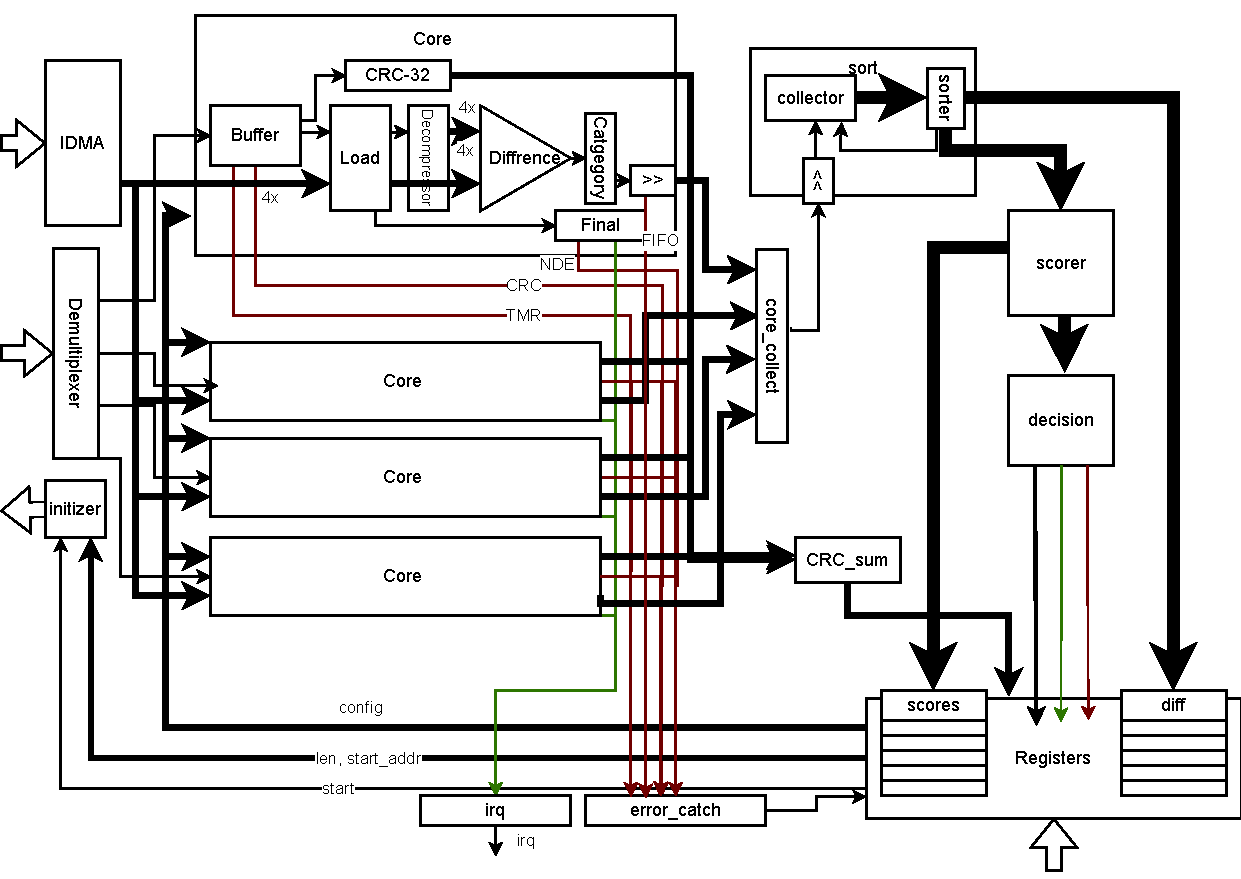
\includegraphics[width=1\textwidth]{AI_compare.pdf}
	\caption{Architektura komponentu klasyfikatora}
\end{figure}
\FloatBarrier %zatrzymanie przenoszenia rysunku

Moduł odbiera dane za pomocą interfejsu strumieniowego z~innego komponentu odpowiedzialnego za odczyt danych z~nośników zewnętrznych. Aby przyspieszyć operację komparacji, komponent czyta jednocześnie zawartość z~czterech nośników. Zadanie to jest inicjowane przez moduł \textbf{initializer} za pomocą interfejsu \textit{Avalon Stream}. Wspomniany interfejs przekazuje wartości z~odczytu nośnika do komponentu \textbf{demultiplexer}. W~tym interfejsie każdy nośnik ma dedykowany przedział bitów, które przechowują odczytane bajty z~pamięci masowej.

Dane uzyskane z~transakcji są rozdzielane do rdzeni \textit{core}, aby tam trafiał ciąg bajtów związany z~jednym nośnikiem. W~rdzeniu dane są sprawdzane pod względem poprawności (w tym wyliczanie \textit{CRC} \cite{Wiki:CRC}), po czym przekazywany jest dalej profil nagrania odczytanego z~nośnika. Później, za pomocą modułu wewnętrznego DMA \textit{IDMA}, dane są pobierane ze specjalnej pamięci \textbf{AI\_RAM}. Zawiera ona profil słowa odebranego przez system. Następnie odbywa się dekompresja danych z~nośnika za pomocą algorytmu opisanego w~rozdziale 3.2.3. Po dekompresji porównywane są cztery próbki profilu na raz, po czym moduł dodaje do obliczonej różnicy kategorię i~przekazuje tę informację do modułu \textbf{core\_collector}.

Za pomocą systemu kolejek dane są zbierane z~rdzeni i~spośród nich wybierane są w~bloku \textbf{collector} osiem najmniejszych różnic. Jeżeli moduł otrzymuje 256 wartości, przekazuje je do bloku \textbf{sorter}, po czym ponawia odbieranie danych. W~module \textit{sorter} różnice są sortowane i~przekazywane jednocześnie do tablicy różnic w~rejestrach oraz do modułu \textbf{scorer}, gdzie danym różnicom przydziela się punkty zgodnie z~algorytmem klasyfikatora. Wyniki wspomnianych operacji są przekazywane do modułu rejestrów.

Finalnie moduł \textbf{decision} podejmuje decyzję, po czym przekazuje ją do modułu rejestrów. Dzięki temu procesor ma dostęp do szczegółowych informacji na temat wykonanej operacji. Rejestry te są udostępniane za pomocą interfejsu \textit{Avalon Memory Mapped}. Procesor inicjuje komparację, zapisując odpowiednie parametry w~rejestrze, po czym czeka na przerwanie, które informuje o~zakończeniu operacji. Zdarzenie to jest raportowane wówczas, gdy wszystkie rdzenie ogłoszą zakończenie operacji. Uruchomienie klasyfikatora powoduje powrót modułów wewnątrz komponentu do stanu wyjściowego.

Komponent również zbiera informacje o~błędach z~podmodułów, takich jak błąd CRC nośnika, zbyt długie czekanie na odpowiedź od nośnika (\textit{Too Many Retries TMR}), brak wykrycia końca odczytywanego zakresu (\textit{No Detected End NDE}), błąd kolejki (\textit{FIFO}). Błędy te, z~rdzeni, są zbierane przez blok \textbf{error\_catch} i~przekazywane do rejestrów, dzięki czemu program procesora może sprawdzić informacje o~błędzie klasyfikatora. Dla błędów również zgłaszane jest przerwanie.

Dodatkowo istnieje mechanizm sprawdzenia sumy CRC-32 IEEE-802.3 \cite{CRC32} z~odczytu dla każdego nośnika. Pozwala on na dodatkowe sprawdzenie, czy odebrane dane z~nośników są z~dużym prawdopodobieństwem żądanym modelem. Moduł \textbf{CRC\_sum} zbiera obliczone CRC z~rdzeni, po czym ich sumę przekazuje do rejestrów. Zdecydowano się na zastosowanie sumy, aby uniezależnić system od kolejności włożenia nośników do slotów.




\subsubsection{Demultiplekser  i~inicjalizator}

Moduł \textbf{demultiplexer} przydziela odebrane dane z~komponentu obsługującego nośniki danych rdzeniom. Jeden rdzeń otrzymuje po przejściu pakietu przez ten moduł dane tylko z~jednej pamięci zewnętrznej. Odbiera on strumień o~szerokości 40 bitów przez interfejs \textit{Avalon Stream} pochodzący z~zewnętrznego komponentu. Dane te mają strukturę określoną na rys. 4.11.

\begin{figure}[h]
	\centering
	\begin{tabular}{|r|r|r|r|r|r|r|}
		\hline
		Wartość & Zarezerwowane & Czy dla  & Dane dla  & Dane dla  & Dane dla  & Dane dla  \\
		 		&  				& rdzenia  & rdzenia 1 & rdzenia 2 & rdzenia 3 & rdzenia 4 \\
		 		&				& są dane  & 		   & 		   & 		   &			\\
		\hline
		Zakres & [39:36] & [35:32] & [31:24] & [23:16] & [15:8] & [7:0]\\
		\hline
	\end{tabular}
	
	\caption{Pakiet informacji otrzymywany podczas jednej transakcji \textit{Avalon Stream} od komponentu obsługującego nośniki.}
\end{figure}
\FloatBarrier %zatrzymanie przenoszenia rysunku

Bity w~zakresie [35:32] odpowiadają za wskazanie, czy dla danego rdzenia były wysyłane dane. Jeżeli bit 35 jest w~stanie wysokim, dane były przesyłane do rdzenia 4; dla 34 bitu dotyczyło to rdzenia 3, itd. Bity [31:0] odpowiadały za przesyłanie danych, gdzie każdy bajt tej zawartości był zarezerwowany dla innego źródła - tak jak w~tabeli 4.11. Pozostałe bity są ignorowane.

Zgodnie ze wskazaniami zakresu [31:32] na interfejsach strumieniowych składających się z~sygnałów \textit{data} i~\textit{rdy} wystawiano odpowiednim rdzeniom dane wycięte z~odebranego pakietu danych. Interfejsy te nie wymagają \textit{handshake}'u tak jak \textit{Avalon Stream} (\textit{avs\_s2}). Do rdzenia 1 podłączony jest interfejs \textit{data1}, do drugiego \textit{data2}, itd. Posiadają one pole danych o~szerokości jednego bajta oraz odpowiadający sobie sygnał \textit{rdy} (dla \textit{data1} \textit{data1\_rdy}, itd.).

Komponentem za inicjację odczytu z~pamięci jest blok \textbf{initializer}. Moduł po otrzymaniu sygnału \textit{init} z~modułu rejestrów wystawia do komponentu zarządzającego pamięciami zewnętrznymi przez interfejs \textit{Avalon Stream} (\textit{avs\_s1}) 40-bitową komendę w~postaci opisanej na rys. 4.12.

\begin{figure}[h]
	\centering
	\begin{tabular}{|r|r|r|r|r|r|r|}
		\hline
		Wartość & Komenda & Adres sektora   & Długość odebranych danych (w kB) \\
		\hline
		Zakres & [39:32] & [31:16] & [15:0] \\
		\hline
	\end{tabular}
	
	\caption{Pakiet informacji wysyłany podczas jednej transakcji \textit{Avalon Stream} do komponentu obsługującego nośniki.}
\end{figure}

Podczas wykonywania polecenia w~polu \textit{komenda} wystawia się wartość 0x0. Prawdziwy adres sektora wyznaczany jest poprzez przemnożenie wartości pola adresu przez 256. Pozwala to na uzyskanie dostępu do dużej przestrzeni adresowej, a~zatem na obsługę nośników o~pojemności nawet 8 GB. Rozmiar taki jest wystarczająco duży jak na zastosowania w~urządzeniach klasy embedded. Wartości te są ustalane na podstawie rejestrów konfiguracyjnych komponentu: \textit{len} i~\textit{start\_addr}.

Moduł może także otrzymać informację o~błędzie z~modułu \textit{error\_catcher} za pomocą zbiorczych sygnałów błędów \textit{tmr}, \textit{crc}, \textit{nde}, \textit{fifo}. Wysyła się wówczas komendę 0xFF z~wyzerowanym adresem i~długością danych po to, aby zatrzymać strumień wartości z~nośników.


\subsubsection{Wewnętrzne DMA \textit{IDMA}}

Aby rdzeń mógł ładować dane z~pamięci \textit{AI\_RAM}, stworzono moduł \textbf{IDMA} (\textit{Inside Direct Access Memory}), który czyta dane z~pamięci RAM na żądanie rdzeni. Każdy rdzeń ma wyprowadzony do wspomnianego komponentu interfejs składający się z~sygnałów \textit{addr} (o szerokości 16 bitów), \textit{data} (32-bitowy) oraz jedno-bitowych \textit{read} i~\textit{rdy}. Rdzeń wystawia adres, z~którego ma być odczytana wartość wraz z~stanem wysokim na \textit{read}, po czym czeka na odpowiedź w~postaci jedynki na \textit{rdy} i~zawartości pamięci w~\textit{data}.

Moduł komunikuje się z~pamięcią \textit{AI\_RAM} za pomocą dwóch interfejsów strumieniowych \textit{Avalon Stream}: \textit{avs\_s2} z~danymi i~\textit{avm\_m2} z~adresami. Oba mają szerokość 64 bitów - najmłodsze 32 bity są zarezerwowane dla jednej transakcji, a~pozostałe dla drugiej. Pamięć RAM pozwala więc na odczyt 2 wartości na raz przez \textit{dual port}, co przyspiesza czytanie danych przez rdzenie, a~tym samym obliczenia.

Schemat działania modułu, będącego prostym automatem stanów, znajduje się na rys. 4.13.

\begin{figure}[h]
	\centering
	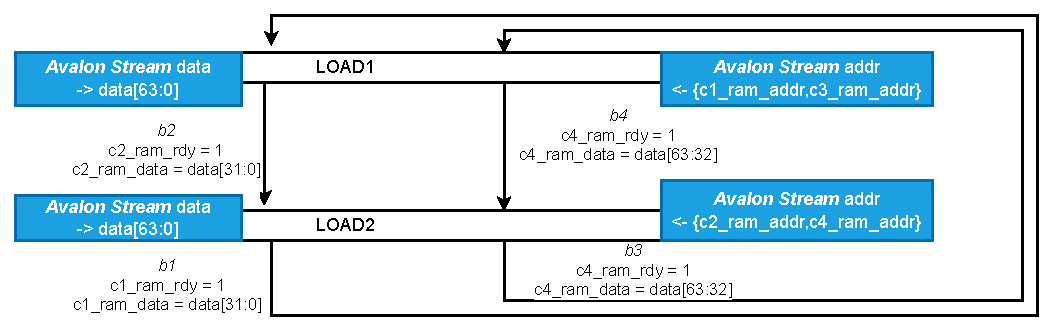
\includegraphics[width=1\textwidth]{IDMA.pdf}
	\caption{Architektura rdzenia komponentu klasyfikatora}
\end{figure}
\FloatBarrier %zatrzymanie przenoszenia rysunku

W stanie \textit{LOAD1} moduł odbiera dane z~interfejsu strumieniowego, jednocześnie wystawiając adres do \textit{DMA} pochodzący z~rdzeni 1 i~3 (na podstawie interfejsów \textit{c1\_ram} i~\textit{c3\_ram}), buforując informacje o~transakcji w~rejestrach \textit{b1} i~\textit{b3}. Jeżeli zbuforowano żądanie w~\textit{b2}, wystawiane są do drugiego rdzenia najmłodsze 32 bity odczytane z~\textit{AI\_RAM}, zaś w~przypadku \textit{b4} wysyła się najstarsze 32 bity do czwartego rdzenia. Przeciwnie, w~przypadku następnego stanu \textit{LOAD2}, moduł wraca do stanu pierwotnego.

Taki układ pozwala na ograniczenie maksymalnego czasu oczekiwania na koniec transakcji do 3 cykli dla rdzenia.

\subsubsection{Budowa rdzenia \textit{AI\_core}}

Budowa jednego z~czterech rdzeni znajdujących się w~komponencie ilustruje rys. 4.14. Dane po interfejsie strumieniowym (określonym w~4.5.2) trafiają do modułu \textbf{wait}, który buforuje dane na dwa cykle za pomocą automatu stanów - zabieg ten skraca ścieżki krytyczne. Wartości z~wcześniej wspomnianego modułu trafiają do bloku \textbf{buffer}, gdzie sprawdzane są pod kątem poprawności pakietów danych zarezerwowanych dla nośnika oraz usuwane są bajty związane z~pakietem, przekazując czyste, skompresowane dane dalej.

\begin{figure}[h]
	\centering
	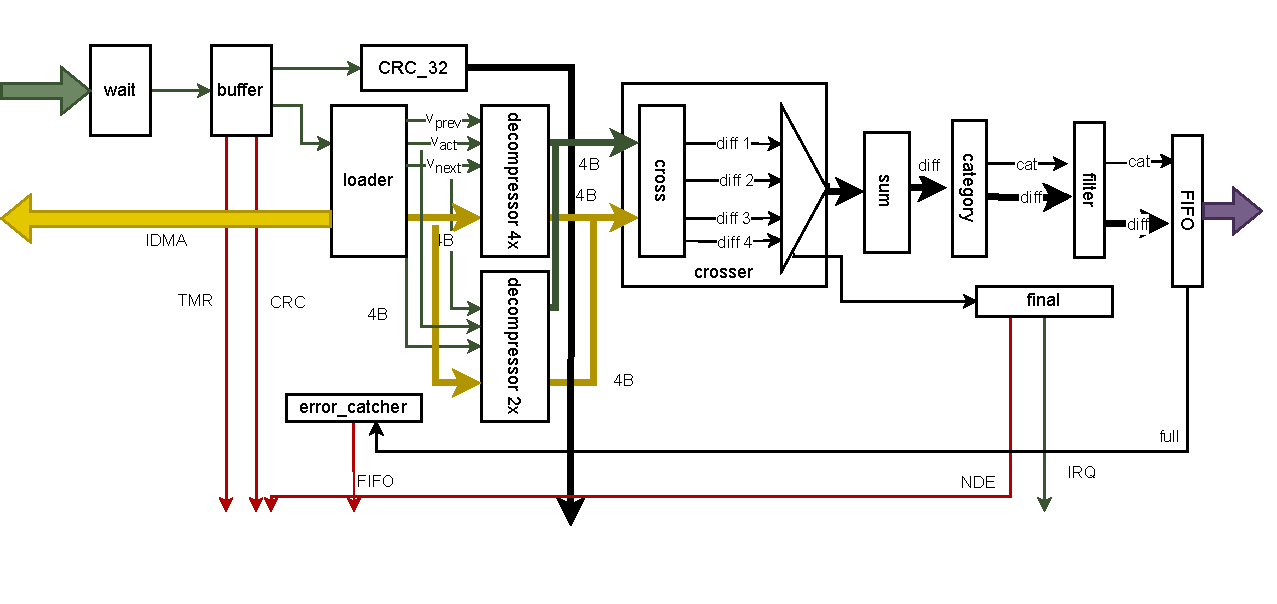
\includegraphics[width=1\textwidth]{AI_core.pdf}
	\caption{Architektura rdzenia komponentu klasyfikatora}
\end{figure}

Dane trafiają stamtąd równocześnie do modułu liczącego \textit{CRC\_32} i~do \textbf{loadera}. \textit{CRC\_32} przekazuje samą wartość bez użycia interfejsu strumieniowego na zewnątrz. \textit{Loader} odpowiada za odczytanie danych z~pamięci \textit{AI\_RAM}, aby dopasować je do odczytanych, skompresowanych danych z~nośnika. Połączony ciąg zdekompresowanych wartości z~nośnika i~z pamięci RAM trafia do jednego z~modułów dekompresujących. Kompresji 2x nie stosuje w~projekcie, więc jej opis zostanie pominięty.

Komponent \textbf{decompressor\_4x} odbiera i~wysyła dane strumieniowo, realizując algorytm określony w~3.2.3. Uzyskuje się w~ten sposób cztery bajty zdekompresowane z~nośnika i~cztery bajty z~pamięci RAM. Jeden bajt w~tym systemie odpowiada jednej próbce profilu, na podstawie której obliczana jest różnica pomiędzy danymi z~modelu a~odebranym dźwiękiem.

Wartości te trafiają do modułu \textbf{crosser}, gdzie ustawia się je przed obliczaniem różnicy. Pozwala to obliczyć ich wartość bezwzględną oraz uniknąć wartości ujemnych, po czym oblicza się sumę różnic między tymi czterema bajtami z~nośnika i~pamięci RAM. Suma ta trafia do modułu \textbf{sum}, gdzie sumuje się uzyskane wartości, aż uzyskano pełną odległość pomiędzy profilem z~modelu a~odebranym dźwiękiem.

Sumie nadaje się kategorię w~module \textbf{category}, a~wyniki o~zbyt dużej różnicy są odrzucane w~module \textbf{filter}. Przed opuszczeniem rdzenia przez dane trafiają one do kolejki \textit{FIFO}.


\FloatBarrier %zatrzymanie przenoszenia rysunku

Rdzeń realizuje koncepcję przetwarzania potokowego.

\subsubsection{Moduły odczytu danych w~rdzeniu}
Dane z~bufora w~module \textit{wait}, po interfejsie strumieniowym (określonym w~4.5.2), trafiają do bloku \textbf{buffer}. Moduł odbiera pojedyncze bajty tworzące pakiety, w~których znajdują się właściwe dane pochodzące z~pamięci zewnętrznej. Budowę pakietu ilustruje rys. 4.15, który przenosi jednocześnie 512-bajtowy sektor czytanego nośnika danych.

\begin{figure}[h]
	\centering
	\begin{tabular}{|r|r|r|r|r|r|r|}
		\hline
		Wartość & Zarezerowane / Stan pakietu & Stan pakietu & Zawartość sektora    \\
		\hline
		Zakres & 1B & 1B & 512B \\
		\hline
	\end{tabular}
	
	\caption{Pakiet zawierający pełny sektor nośnika przesyłany do rdzenia}
\end{figure}

Pierwsze dwa bajty pakietu sprawdzane są pod kątem wystąpienia błędu. Komponent zarządzający nośnikami wysyła jako stan 0xFE, gdy czas oczekiwania na nośnik jest zbyt długi, lub 0xFD w~przypadku błędu przy odczycie CRC. Jeżeli w~którymkolwiek z~powyższych bajtów wystąpi taka wartość, wysyłany jest odpowiedni sygnał informujący o~błędzie (\textit{tmr} lub \textit{crc}).

Bajty te są odrzucane, a~w~przypadku niewystąpienia błędu na kolejne interfejsy wystawiane są pozostałe 512 bajtów paczki. Jeden interfejs jest połączony z~podmodułem CRC (\textit{CRC\_32}), a~drugi z~modułem \textit{loader}. Ze względu na brak handshake'u, wysłanie jednocześnie informacji do dwóch modułów jest proste i~nie wymaga oczekiwania na odpowiedź, a~jedynie wystawienia sygnału \textit{rdy} i~wartości w~polu \textit{data} przez jeden cykl zegarowy.

Moduł \textbf{CRC\_32} został wygenerowany za pomocą zewnętrznego narzędzia \textit{Online generator for CRC HDL code} \cite{CRC_32}. Moduł pozwala na proste podłączenie do zastosowanego wcześniej interfejsu strumieniowego, gdyż stosuje on taki sam interfejs do ładowania do niego danych.

\textbf{Loader} łączy dane z~pamięci \textit{AI\_RAM}, stosując automat stanów opisany na rys. 4.16.

Moduł czeka w~stanie \textit{IDLE} na transakcje strumieniową po czym dokonuje ustalenia wartości aktualnej, poprzedniej i~przyszłej. Odebrane wcześniej dane z~pamięci \textit{AI\_RAM} są przepisywane do rejestrów dla aktualnych wartości. Na podstawie licznika moduł wystawia do \textit{IDMA} żądanie odczytu danego adresu pamięci (tak aby dopasować go do odebranych wcześniej danych). Po otrzymaniu wartości automat przechodzi do stanu \textit{READ} gdzie wystawia na interfejs blokowi \textit{decompressor} informacje z~odczytu pamięci (\textit{last1},\textit{last2},\textit{last3} i~\textit{last4}) oraz te które potrzebne będą dalej do dekompresji wartości z~nośnika (\textit{next\_mem}, \textit{mem} i~\textit{last\_mem}).

\begin{figure}[h]
	\centering
	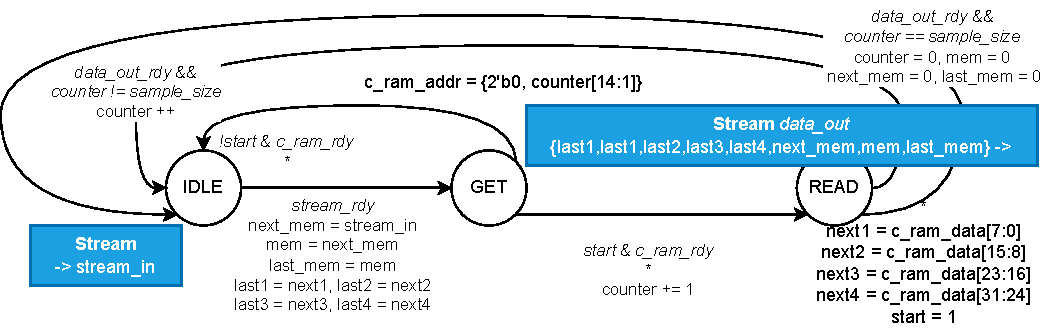
\includegraphics[width=1\textwidth]{loader_fsm.pdf}
	\caption{Automat stanów modułu \textit{loader}}
\end{figure}
\FloatBarrier %zatrzymanie przenoszenia rysunku



Ze względu na stosunkowo wolne odczytywanie danych z~nośnika pakiety nie przepadają gdyż cały cykl dla zastosowanego w~tym projekcie \textit{IDMA} może trwać 5 cykli. Dane z~pamięci zewnętrznej są odczytywane zdecydowanie wolniej (jeden bajt odczytywany jest przez 12 cykli).

\subsubsection{Moduły dekompresujące i~obliczające różnicę w~rdzeniu}

Dane z~modułu \textit{loader} trafiają do bloku \textbf{decompressor 4x}. Moduł otrzymuje 64-bitową wartość zgodną z~rys. 4.16. Dzięki temu, że dekompresor ma dostęp do wartości aktualnej, bieżącej i~przyszłej próbki, zadanie dekompresji realizowane jest przez prosty automat stanów, który buforuje odebrane wartości, po czym wykonuje obliczenia zgodne z~algorytmem w~3.2.3. Zamiast mnożeń stosuje on odpowiednie przesunięcia bitowe - 0.5 to przesunięcie o~1, 0.25 przesuwa o~2 itd. Wartości odebrane z~pamięci są przekazywane na interfejs wyjściowy.

Założono, że wartości próbek na potrzeby algorytmu KNN są nieujemne, więc ignoruje się potrzebę obsługi takich liczb. Finalnie automat wystawia na interfejsie dane w~postaci takiej jak na rys. 4.17. Zwracana wartość jest 64-bitowa.

\begin{figure}[h]
	\centering
	\begin{tabular}{|r|r|r|r|r|r|r|r|r|}
		\hline
		Wartość & Zdeko. & Zdeko. & Zdeko. & Zdeko. & War 1.  & War. 2  & War. 3  & War. 4\\
				& war. 1  & war. 2  & war. 3  & war. 4	& z~RAM & z~RAM & z~RAM & z~RAM\\
		\hline
		Zakres & [63:56] & [55:48] & [47:40] & [39:32] & [31:24] & [23:16] & [15:8] & [7:0] \\
		\hline
	\end{tabular}
	
	\caption{Pakiet informacji wysyłana z~komponentu dekompresującego, skróty \textit{Zdeko.} - zdekompresowany, \textit{War.} - wartość }
\end{figure}
\FloatBarrier %zatrzymanie przenoszenia rysunku

Wartości te trafiają do bloku \textbf{crosser} (także z~użyciem interfejsu strumieniowego określonego w~rozdziale 4.5.2). Jest to prosty automat stanów, który po odebraniu transakcji w~stanie \textit{IDLE} wewnętrznie przestawia liczby, zapisując je do rejestrów wewnętrznych. Dzięki temu w~następnym stanie (\textit{ABS}) uzyskuje wartość bezwzględną różnicy odpowiadających sobie próbek profilu (zdekompresowana wartość 1 z~wartością 1 z~pamięci RAM, zdekompresowana wartość 2 z~wartością 2 z~pamięci RAM itd.). W~finalnym stanie \textit{FINAL} moduł zwraca sumę tych różnic przez interfejs strumieniowy o~szerokości 10 bitów (tak aby mogła się w~nim zmieścić maksymalna suma różnic 4 liczb 8-bitowych).

Kolejnym modułem przetwarzającym dane po obliczeniu różnicy dla pakietów 4B danych jest \textbf{sum}, do którego dane trafiają strumieniowo. Po otrzymaniu transakcji uzyskana wartość jest dodawana przez sumator do rejestru. Licznik oblicza, ile różnic trafiło do modułu. Jeżeli zostanie przekroczony zakres ustawiony za pomocą rejestru konfiguracyjnego \textit{sample\_size} (określa rozmiar profilu w~kilobajtach po kompresji), ustawianego przez procesor, wystawia się na interfejsie wyjściowym sumę obliczoną do tamtej pory. Gdy transakcję zakończono, suma jest zerowana. W~ten sposób oblicza się sumę dla jednego profilu dźwięku pobranego z~pamięci. Profile te są ułożone w~zawartości nośnika po kolei, stąd możliwe jest analizowanie wielu profili przez jeden rdzeń. Uzyskana suma jest wartością 32-bitową, ale realnie używano jedynie 24 bitów.

Wynika to z~faktu, iż maksymalna różnica pomiędzy tablicą 8 bitowych elementów o~całkowitym rozmiarze 32 kB z~dedykowanej pamięci RAM klasyfikatora a~zdekompresowanym profilem z~modelu wynosi $32 * 1024 * \Delta_{max} = 32 * 1024 * 255 = 8 355 840$. Liczba ta jest mniejsza niż $2^{24} = 16 777 216$.

Jednym z~modułów sprawdzających, czy zakończono komparację w~danym rdzeniu, jest \textbf{final}. Nasłuchuje on transakcji strumieniowych pomiędzy blokiem \textit{crosser} a~\textit{sum}, a~gdy wykrywa transakcję, moduł zeruje wewnętrzny licznik, w~przeciwnym wypadku odlicza aż do przekroczenia granicznej wartości 500000. Gdy rejestr ten osiąga 499998, sprawdza, czy moduł odczytał prawidłową liczbę transakcji na podstawie rejestru konfiguracyjnego \textit{len}, ustawianego przez procesor, po czym ustala długość strumienia danych w~sektorach. Na potrzeby tego modułu wartość ta jest mnożona przez 512, aby uzyskać z~liczby sektorów liczbę bajtów potrzebnych do pełnego odczytu żądanej zawartości. Gdy wczytano mniej danych niż wskazuje rejestr, wysyła się sygnał błędu \textit{NDE}, w~przeciwnym przypadku sygnał \textit{irq} do rdzenia.

\subsubsection{Moduły klasyfikujące w~rdzeniu}

Uzyskana suma różnic, będąca odległością pomiędzy profilami dla algorytmu \textit{KNN}, trafia do modułu \textbf{category}. Do 24-bitowej sumy blok dodaje kategorię, tworząc 32-bitową wartość zgodnie z~tabelą na rys. 4.18.

\begin{figure}[h]
	\centering
	\begin{tabular}{|r|r|r|r|r|r|r|r|r|}
		\hline
		Wartość & 4'b0100 & Kategoria (wartość z~licznika kategorii) & Odległość (suma różnic)\\
		\hline
		Zakres & [31:28] & [27:24] & [23:0] \\
		\hline
	\end{tabular}
	
	\caption{Pakiet tworzony przez moduł \textit{category}}
\end{figure}

Licznik, będący rejestrem wewnętrznym, liczy liczbę transakcji na interfejsie wejściowym. Gdy ta wartość jest równa zawartości rejestru \textit{packet\_size} (określającego, ile profili dla danego dźwięku znajduje się na nośniku), ustawianego przez procesor, licznik wyznaczający numer kategorii wówczas się inkrementuje. Moduł obsługuje maksymalnie 8 rodzajów wykryć (kategorii). Wartość rejestru liczącego wówczas się zeruje. Każda transakcja wejściowa kończy się wysłaniem dalej po interfejsie strumieniowym pakietu opisanego na rys. 4.12.

Suma z~kategorią trafia do modułu \textbf{filter}, który odrzuca wartości sum większe niż określony próg przez rejestr konfiguracyjny \textit{max}, ustawiany z~poziomu procesora. Wartość uzyskana z~bloku \textit{category} jest przekazywana, o~ile spełnia warunki sprawdzane przez rejestr. Jeżeli suma była większa, sumę podmieniano wartością 0xFFFFFF. Dzięki temu minimalizowano prawdopodobieństwo, że niespełniająca warunków odległość może być uznana przez klasyfikator w~dalszej analizie za interesującą. Moduł, po otrzymaniu transakcji na interfejsie wyjściowym, wysyła dane strumieniowo dalej do kolejki synchronicznej w~module \textbf{FIFO}. Wspomniana kolejka może przechowywać maksymalnie 64 słowa 32-bitowe.

Implementacja synchronicznego \textbf{FIFO} pochodzi z~zewnętrznego źródła \cite{FIFO:source}. Rejestr FIFO pozwala na bezpośrednie podłączenie wejścia do interfejsu strumieniowego stosowanego w~tym rdzeniu. Sygnał \textit{full} jest podłączony do modułu \textbf{error\_catcher}. Jeżeli wykrywa on zmianę ze stanu wysokiego na niski sygnału informującego o~tym, że kolejka jest pełna, wysyła impuls do modułu \textit{error\_catcher} znajdującego się poza rdzeniem. Dane z~kolejki można pobierać za pomocą interfejsu składającego się z~sygnałów jednobitowych \textit{read}, \textit{full} i~\textit{empty} oraz 32-bitowego \textit{data\_out}. Działa on analogicznie do natywnego interfejsu BRAM - po wystawieniu sygnału \textit{read} w~następnym cyklu zegarowym pojawi się pobrana z~kolejki wartość.


\subsubsection{Moduły zbierające i~sortujące dane}
Modułem zbierającym dane z~kolejek wyjściowych rdzeni jest automat stanów \textbf{core\_collect}. Korzysta on z~algorytmu \textit{round robin} \cite{RoundRobin}. Każdy rdzeń ma swój dedykowany stan, w~którym moduł sprawdza na interfejsie kolejki, czy nie jest pusta, korzystając z~sygnału \textit{empty}. Gdy wykryje na nim stan niski, zapisuje tę informację w~dedykowanym dla rdzenia rejestrze oraz wysyła sygnał \textit{read}. W~następnym stanie odczytana z~kolejki wartość jest przekazywana na interfejs strumieniowy, taki jak stosowany wcześniej w~rdzeniach, do kolejki wyjściowej. Do wartości dodaje się 2-bitowy numer nośnika na podstawie tego, z~którego rdzenia pochodziła. Schemat nowo powstałego pakietu ilustruje rys. 4.19.

\begin{figure}[h]
	\centering
	\begin{tabular}{|r|r|r|r|r|r|r|r|r|}
		\hline
		Wartość & 2'b01 & Numer nośnika & Kategoria & Odległość (suma różnic) \\
		\hline
		Zakres & [31:30] & [29:28] & [27:24] & [23:0] \\
		\hline
	\end{tabular}
	\caption{Pakiet tworzony przez moduł \textit{core\_collect}}
\end{figure}
\FloatBarrier %zatrzymanie przenoszenia rysunku

Kategorię i~odległość przenosi się bez zmiany z~kolejki. Automat w~stanie \textit{LOAD1} zapisuje stan \textit{FIFO} 1 i~przesyła w~przypadku wcześniejszego zapisania odpowiedniego rejestru dane związane z~odczytem kolejki rdzenia 4. Dla \textit{LOAD2} wpisuje się informację o~zawartości \textit{FIFO} z~rdzenia 2, zaś wystawia się na interfejs odczyt z~kolejki bloku \textit{core} 2. Podobna reguła obowiązuje w~pozostałych stanach \textit{LOAD3} i~\textit{LOAD4}. Moduł po zakończeniu stanu \textit{LOAD4} wraca do \textit{LOAD1}. Czeka on też na to, aby kolejka wyjściowa - również o~rozmiarze 64 słów - podłączona do interfejsu wyjściowego była niepełna; w~innym przypadku nie odczytuje danych z~kolejek rdzeni.

Dane wystawione z~modułu \textit{core\_collector} trafiają strumieniowo do wrappera \textbf{sort} z~dwoma modułami - \textbf{collector} i~\textbf{sorter}. Moduł \textbf{collector} odpowiada za wybranie najlepszych 8 dopasowań, czyli najmniejszych sum różnic. Automat stanów zastosowany w~tym module znajduje się na rys. 4.20.

\begin{figure}[h]
	\centering
	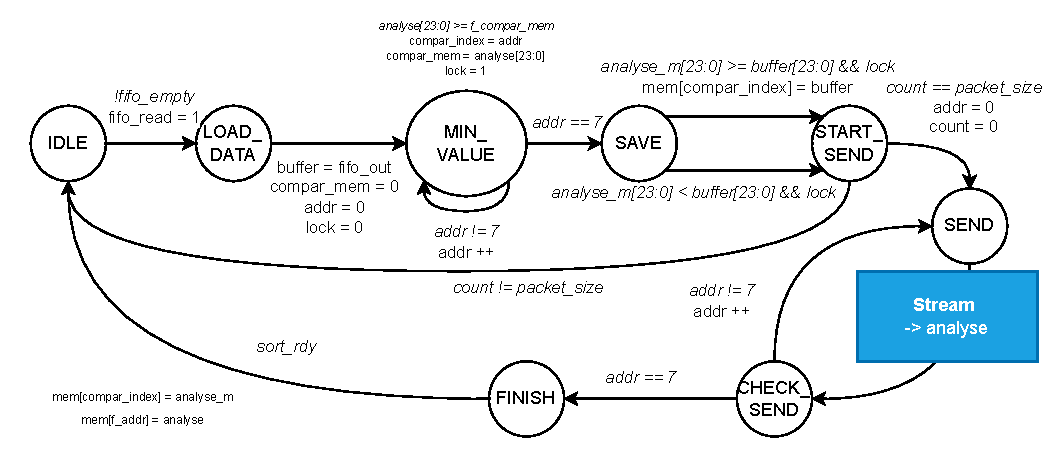
\includegraphics[width=1\textwidth]{collector.pdf}
	\caption{Automat stanów \textit{collector}}
\end{figure}
\FloatBarrier %zatrzymanie przenoszenia rysunku

Najpierw odczytuje pakiet z~kolejki (o ile kolejka była niepusta), stosując interfejs dla kolejek z~rozdziału 4.5.7. Automat zeruje swoje rejestry wewnętrzne, po czym rozpoczyna wyszukiwanie największej wartości w~zbiorze 8 zapisanych wewnątrz modułu. Po przeszukaniu wszystkich 8 wartości moduł sprawdza, czy ta wartość jest większa od odebranej w~stanie \textit{IDLE}. Gdy spełniono ten warunek, moduł podmienia to pole w~tablicy. Aby zbyt często nie wysyłać pakietów, moduł wystawia dane do bloku \textit{sorter} tylko co liczbę odebranych pakietów, jaką wskazuje parametr \textit{packet\_size} ustawiany przez procesor. Gdy osiągnięto tę wartość, moduł przechodzi do procedury przesyłu interfejsem strumieniowym zbioru 8 najmniejszych odległości. W~innym przypadku wraca do \textit{IDLE}. Finalnie, po przesyle, czeka na to, aż pod-komponent sortujący zwróci informację o~zakończeniu sortowania, po czym automat wraca do stanu \textit{IDLE}.

Dzięki takiej budowie moduł odrzuca wszystkie zbyt duże odległości i~zostawia jedynie informacje potrzebne klasyfikatorowi.

Dane z~modułu \textit{collector} przechodzą do modułu \textbf{sorter}, będącego prostym \textit{FSM} sortującym odebrany ciąg 8 pakietów z~najmniejszymi odległościami pomiędzy profilami. Najpierw w~stanie \textit{IDLE} jest ona podczas transakcji po interfejsie strumieniowym zapisywana do dedykowanych rejestrów tworzących tablicę. Gdy odebrany został cały zestaw 8 najmniejszych różnic, moduł przechodzi do stanu \textit{MIN\_VAL}. Moduł szuka tam najmniejszej wartości z~zapisanych w~pamięci. Następnie zapisuje jej pozycję, po przeszukaniu całego zbioru (na jedną wartość jeden cykl). Po przeszukaniu całego zapisanego zbioru moduł przechodzi do stanu \textit{SEND}, gdzie wystawia na interfejs strumieniowy znalezioną wartość, jednocześnie nadpisując pole w~tablicy maksymalną wartością 32-bitową (0xFFFFFFFF). Licznik wysłanych liczb jest inkrementowany. Następnie wraca do stanu \textit{MIN\_VAL}, o~ile nie wykryto, że wysłano 8 paczek. Gdy okazuje się, że wystawiono wszystkie wartości z~tablicy, wysyła z~powrotem do modułu \textit{collector} sygnał o~zakończeniu operacji sortowania, po czym automat wraca do stanu \textit{IDLE}.

Dane po interfejsie strumieniowym trafiają do modułu \textit{scorer} oraz pod-komponentu odczytu rejestrów, dzięki czemu efekt tego sortowania może być sprawdzany przez procesor.

\subsubsection{Moduły decyzyjne}

Po opuszczeniu wrappera dane są analizowane przez \textbf{scorer}. Moduł w~stanie \textit{IDLE} odbiera pakiet z~sumą, po czym rozbija ją na kategorię i~odległość, zapisując je w~dedykowanych rejestrach. Następnie przechodzi do stanu \textit{CLEAR}, gdzie w~przypadku odebrania pierwszego bajtu zestawu 8 najmniejszych różnic, czyszczona jest z~zawartości tablica z~wynikami punktowymi. Potem, w~stanie \textit{SAVE}, zgodnie z~licznikiem transakcji przydzielane są punkty według algorytmu 3.2.4. Ustalona liczba jest dodawana do rejestru dedykowanego dla jednej z~8 kategorii, jakie są rozpoznawane przez klasyfikator. W~przypadku odebrania 8 pakietów, moduł przechodzi do stanu \textit{SEND}, gdzie wystawia 2 rejestry z~obliczoną liczbą punktów dla każdej kategorii. Rysunek 4.21 pokazuje zawartość wspomnianych rejestrów.

 \begin{figure}[h]
 	\centering
 	\begin{tabular}{|r|r|r|r|r|r|r|r|r|}
 		\hline
 		Zakres & [31:24]& [23:16]& [15:8] & [7:0]\\
 		\hline
 		reg1 &  kategoria 1 & kategoria 2 & kategoria 3 & kategoria 4 \\
 		\hline
 		reg2 & kategoria 5 & kategoria 6 & kategoria 7 & kategoria 8 \\
 		\hline
 	\end{tabular}
 	
 	\caption{Rejestry wynikowe modułu \textit{scorer} gdzie określono pozycję punktów w~rejestrach dla danej kategorii}
 \end{figure}
 
Rejestry są udostępnione przez komponent \textit{av\_reader}, dzięki czemu mogą być one odczytane przez program procesora. Gdy wartość rejestrów jest nadpisana, wystawia się sygnał \textit{rdy} poza moduł. Moduł po zapisaniu tych rejestrów wraca do stanu \textit{IDLE}.

Ostatnim modułem przetwarzającym dane jest \textbf{decision}. Ponownie jest to automat stanów, który czeka na gotowość ze strony modułu \textit{scorer}. Następnie w~rejestrach wystawionych przez poprzedni moduł sprawdza po kolei (jeden wynik na cykl zegara), która liczba punktów jest największa. Po wybraniu największego wyniku sprawdzane jest, czy wartość spełnia warunki określone przez rejestr konfiguracyjny \textit{min}, ustawiany przez procesor. Pozwala to na odrzucanie zbyt słabych klasyfikacji, zgodnie z~rozważaniami w~rozdziale 3.2.4. Wartość po zatrzaśnięciu jest przekazywana do modułu odczytu rejestrów bez użycia interfejsu strumieniowego, aby można było ją sprawdzać z~poziomu programu.
 
 
\subsubsection{Rejestry sterujące komponentem}

Komunikację komponentu z~procesorem umożliwiają moduły \textbf{av\_reader} i~\textbf{av\_writer}. Udostępniają one rejestry przy użyciu interfejsu \textit{Avalon Memory Mapped}, na potrzeby sprawdzenia stanu operacji lub skonfigurowania komponentu tak, aby wykonał żądaną operację na odpowiednich danych. Tabela na rys. 4.22 prezentuje rejestry udostępniane przez wspomniane wcześniej moduły. Wartości możliwe do odczytu nie mogą być nadpisane z~poziomu programu procesora.

 \begin{figure}[h]
	\centering
	\begin{tabular}{|r|r|r|}
		\hline
		Adres & Znaczenie rejestru & Wartości \\
		\hline
		0x14 &  Zwolnienie przerwania & Nadpisanie jakiejkolwiek wartością  \\
			 &						  & powoduje zwolnienie przerwania	   \\
		\hline
		0x4 &  Minimalny limit punktów & Tylko do zapisu: [3:0] - minimalny próg \\
			&						   & punktowy dla klasyfikatora - parametr \textit{min} \\
 		\hline
 		0x8 & Rozmiary pakietów danych & Tylko do zapisu: [23:16] (parametr \textit{packet\_size}) \\	
 		& 						   & - liczba profili dla danej \\
 		& 						   & kategorii dla jednego nośnika  \\
 		&						   & [14:0] - rozmiar skompresowanego \\
 		&						   & profilu w~kilobajtach	\\
 		\hline
		0xa & Maksymalna odległość	   & Zapis : bity [23:0] (parametr \textit{max})\\
		& między profilami oraz	   & Odczyt : [3] błąd kolejek fifo, \\
		& komunikaty o~błędach     & [2] Nie wczytano wszystkich informacji \\
		& 	   					   & w~odpowiednim czasie \textit{NDE} \\
		&						   & [1] zbyt długi czas oczekiwana na nośnik \textit{TMR} \\
		&						   & [0] błąd CRC nośnika	\\
		
		\hline 
		0x0 & Inicjacja komponentu	   & Tylko do zapisu - zapis inicjuje operację \\
			&						   & wysyłając sygnał \textit{init} oraz \\
			&						   & nadpisuje rejestry kofiguracyjne: \\
			&						   & [31:16] (parametr \textit{load\_sector}) \\ 
			&						   & - adres sektora na nośniku z~\\
			&						   & precyzją do 256 \\
			&						   & [15:0] - rozmiar ładowanych \\ 
			&						   &  danych w~sektorach z~\\
			&						   & jednego nośnika\\
			\hline
		0x10& Kompresja				   & Zapis [0] - 1'b1 kompresja x4 , \\
			&						   & 1'b0 - kompresja x2 \\
		&						   & Odczyt - pakiet o~najmniejszej różnicy	taka jak \\
		&						   & w~4.5.8 \\
		\hline
		0x10 - & Posortowane 8 pakietów od  & Odczyt tak jak w~4.5.8\\
		0x2c & najmniejszej odległości do & \\
		& największej wraz  & \\
		& z~informacjami pobocznymi					 & \\

		\hline
	\end{tabular}
 \end{figure}
\FloatBarrier %zatrzymanie przenoszenia rysunku

 \begin{figure}[h]
	\centering
	\begin{tabular}{|r|r|r|}
		\hline
		Adres & Znaczenie rejestru & Wartości \\
				\hline
		0x30 & Pierwszy rejestr z~wynikami  & Tylko do odczytu tak jak w~4.5.9\\
		& punktowymi (\textit{reg1)}	& \\
		\hline

		
		0x34 & Pierwszy rejestr z~wynikami  & Tylko do odczytu tak jak w~4.5.9\\
		& punktowymi (\textit{reg2)}	& \\
		\hline
		0x38 & Rezultat operacji		& Tylko do odczytu [3:0] - wynik operacji \\
			 & 							& 4'hF - brak wykrycia , \\
			 &							& wartości 0-7 przydzielanych \\
			 &							& kategorii \\
		\hline
		0x3c & Suma sum kontrolnych CRC & Tylko do odczytu [31:0] \\
		\hline
	\end{tabular}
	
	\caption{Rejestry konfiguracyjne komponentu \textit{AI\_comparer}}
\end{figure}
\FloatBarrier %zatrzymanie przenoszenia rysunku

Offset komponentu wyniósł 0x40000 oraz otrzymał numer przerwania 3. Podłączono go do szyny procesora za pomocą narzędzia \textit{Platform Designer}, łącząc \textit{IDMA} z~pamięcią \textit{AI\_RAM}, demultiplekser komponent obsługujący nośniki oraz komponent rejestrów i~przerwanie z~procesorem. Więcej szczegółów związanych z~połączeniem do procesora znajduje się w~załączniku 1. Moduł rejestrów nie wykorzystuje sygnału \textit{byteenable}, stąd nadpisanie jednego rejestru powoduje zmianę wartości całej zawartości, bez względu na to, czy zapisywano tam jeden bajt, czy 4 bajty w~jednej transakcji.

\subsection{Komponent \textit{AI\_RAM}}

Aby szybciej ładować dane do komparacji przez klasyfikator \textit{AI\_comparer}, opracowano specjalną pamięć RAM dual-port o~rozmiarze 32 kB. Procesor ma do niej dostęp pod offsetem 0x10000 i~może z~niej korzystać jak ze zwykłej pamięci RAM. Interfejs komunikacyjny \textit{Avalon Memory Mapped} używany przez nią wspiera sygnał \textit{byteenable}. Do komponentu, za pomocą narzędzia \textit{Platform Designer}, podłączony jest interfejs strumieniowy wejściowy \textit{Avalon Stream} z~\textit{AI\_DMA} (32-bitowy) oraz dwa z~komponentu \textit{AI\_comparer} (z IDMA), jeden z~adresami, drugi z~zwróconymi danymi (64-bitowy).

Interfejs strumieniowy z~\textit{AI\_DMA} posiada dodatkowo sygnały \textit{endofpacket} i~\textit{startofpacket}. Dane z~interfejsu strumieniowego wychodzącego z~\textit{AI\_DMA} trafiają do kolejki, po czym specjalny moduł zapisuje je po kolei, zaczynając od adresu zerowego. Zapis rozpoczyna się od otrzymania pakietu składającego się z~4 bajtów w~jednej transakcji wraz z~sygnałem \textit{startofpacket}, a~kończy się otrzymaniem wartości z~\textit{endofpacket} w~stanie wysokim.

Zgodnie z~rozdziałem 4.5.3, interfejsy wychodzące z~\textit{AI\_comparer} do omawianej pamięci pozwalają na odczyt 2 wartości w~tym samym czasie. Transakcja strumieniowa z~interfejsu, na którym komponent otrzymuje adres, jest rozbijana na 2 operacje odczytu wykonywane za pomocą dwóch wyjść umożliwiających odczyt. Ponieważ jest to pamięć typu \textit{dual port}, operacje te są wykonywane w~tym samym czasie. Odczytane wartości są łączone, po czym wysyłane jedną transakcją z~powrotem do klasyfikatora.

Komponent składa się z~4 bloków pamięci, z~których każdy odpowiedzialny jest za odczyt bajtu dla danego bitu sygnału \textit{byteenable} z~adresu otrzymanego przez interfejs \textit{Avalon MM} slave. Na wyjściu dane są łączone w~jedno wyjście, co pozwala na prostą implementację odczytu pojedynczych bajtów z~poziomu procesora.
\subsection{Komponent \textit{AI\_DMA}}

Schemat komponentu \textbf{AI\_DMA} znajduje się na rys. 4.23.

\begin{figure}[h]
	\centering
	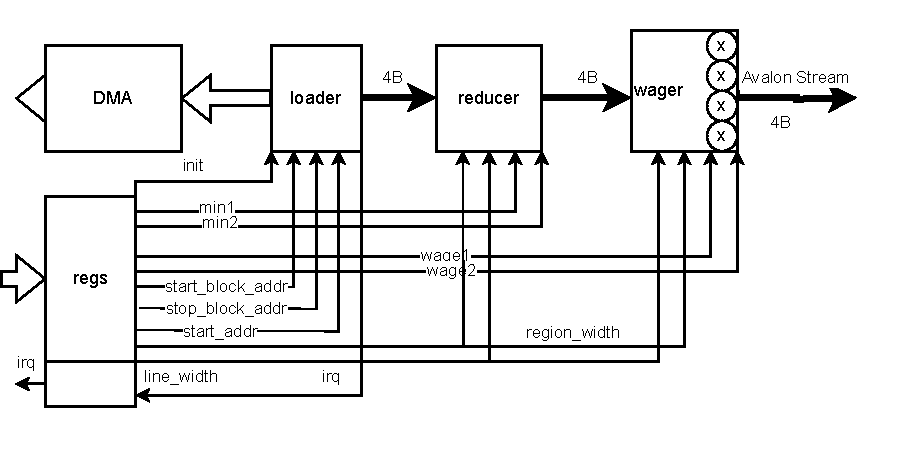
\includegraphics[width=1\textwidth]{AI_DMA.pdf}
	\caption{Schemat komponentu \textit{AI\_DMA}}
\end{figure}

Do czytania danych z~pamięci głównej \textit{RAM} komponent używa tego samego modułu \textit{DMA} co \textit{Signal\_Processor}. Komunikuje się z~nim \textbf{loader}, który czyta dane i~przekazuje je do przetwarzania potokowego, dzięki któremu wartości są przygotowywane do zapisania jako profil dla klasyfikatora. \textbf{Reducer} usuwa z~ładowanych danych próbki, które były zbyt małe (mniejsze niż skonfigurowana wartość minimalna), aby ignorować wpływ nieznacznych niuansów będących potencjalnie szumem. Dane trafiają dalej do modułu \textbf{wager}, gdzie otrzymane próbki są mnożone przez przydzieloną im wagę, aby odzwierciedlić wpływ próbek bez potrzeby angażowania do tego procesora. Procedurę tę zaimplementowano sprzętowo, aby przyspieszyć pomiar cech kluczowych. W~tym projekcie waga była stała dla całego profilu, a~blok \textit{wager} zaimplementowano przyszłościowo pod kątem stworzenia uniwersalnej platformy AI dla urządzeń o~małych zasobach. Dane z~modułu \textit{loader} przez bloki \textit{reducer} i~\textit{wager} płyną interfejsami strumieniowymi typu \textit{Avalon Stream} z~zastosowaniem sygnałów \textit{endofpacket} i~\textit{startofpacket}.

Komponent otrzymał offset 0x0 oraz numer przerwania 10. Podłączony jest za pomocą narzędzia \textit{Platform Designer} do szyny adresowej zarówno \textit{DMA}, jak i~rejestrów oraz wyjścia strumieniowego do pamięci \textit{AI\_RAM}. Pozycje adresów opisuje rys. 4.24.

\begin{figure}[h]
	\centering
	\begin{tabular}{|r|r|r|}
		\hline
		Adres & Funkcja & Zakresy wartości\\
		\hline
		0x0 & Zwolnienie przerwania & Nadpisanie jakąkolwiek wartością \\
		& & tego adresu powoduje \\
		& & wyzerowanie przerwania procesorowego\\
		
		\hline 
		0x4 & Początek bloku danych & [31:0] (parametr \textit{start\_block\_addr})\\
		
		\hline 
		0x8 & Koniec bloku danych & [31:0] (parametr \textit{stop\_block\_addr})\\
		
		\hline 
		0xc & Długość ładowanych danych  & [15:0] (parametr \textit{data\_len})\\
		
		\hline 
		0x10 & Minima & [16] - przesunięcie danych \\
			 &		  & o~2 podczas ładowania  \\
			 &        & [15:8] - minimum 2 (\textit{min1}) \\
			 &		  & [7:0] - minimum 1 (\textit{min2})\\
		
		\hline 
		0x14 & Wagi & [7:0] - waga 1 (\textit{wage1}), \\
			 &      & [15:8] - waga2 (\textit{wage1})\\
			 
		\hline 
		0x18 & Adres rozpoczęcia odczytu & [31:0] (parametr \textit{start\_addr})\\
		
		\hline 
		0x1c & Inicjacja operacji & Nadpisanie tej wartości jakąkolwiek wartością\\
			 & 					  & rozpoczyna operację ładowania danych\\
			 
			 
			 \hline 
		0x20 & Rozmiar linijki profilu & [15:0] (parametr \textit{line\_width})\\
		
		\hline 
		0x24 & Szerokość pierwszego regionu & [15:0] (parametr \textit{region\_width})\\
		\hline
	\end{tabular}
	
	\caption{Rejestry komponentu \textit{AI\_DMA}}
\end{figure}
\FloatBarrier %zatrzymanie przenoszenia rysunku

\textit{Loader} jest automatem stanów. Moduł oczekuje na inicjację z~poziomu rejestrów, po czym rozpoczyna odczyt od adresu rozpoczęcia. \textit{Loader} jest przystosowany do ładowania danych z~bufora cyrkularnego, dlatego należy określić również adresy początku i~końca bloku. Jeżeli podczas ładowania danych z~pamięci blok odczyta dane z~adresu końcowego bloku, moduł przechodzi do adresu początkowego dla bloku. Odczytane 32 bity przez \textit{DMA} zamienia się na 2 wartości 8-bitowe. W~standardowym przypadku są to bity o~pozycjach dla pierwszej liczby [7:0] a~dla drugiej [23:16]. W~przypadku, gdy ustawiono parametr przesunięcia, są to przedziały [9:2] i~[25:18]. Moduł zbiera dane przez 2 takie transakcje, po czym wystawia zebrane wartości na interfejs strumieniowy. Licznik transakcji odlicza ilość odczytów \textit{DMA}, dodając 4 dla każdej z~nich (podczas jednej transakcji odczytuje się 4 bajty), aż do osiągnięcia długości ustawionej w~parametrze. Wówczas zakańcza się odczyt danych oraz wysyła do modułu rejestrów sygnał inicjujący wystawienie przerwania.

Dzięki takiej implementacji komponent może służyć nie tylko do ładowania danych na potrzeby pamięci dedykowanej klasyfikatora, ale także do innych operacji na danych, od których można wyręczyć procesor.

Moduły \textbf{reducer} i~\textbf{wager} są przystosowane do usuwania zbyt małych wartości i~stosowania wag dla dwóch stref w~jednym profilu ładowanym do danych. Profile, tak jak wcześniej ustalono (rozdział 3.2.2), składają się z~linijek. Każda linijka ma taką samą długość i~można je podzielić na dwie strefy - związane ze spektrogramem i~\textit{ZCR} o~stałych rozmiarach, wymagających innego traktowania (innej wartości minimalnej). Parametr \textit{region\_width} pozwala na ustalenie rozmiaru pierwszej strefy, a~drugą strefę stanowią pozostałe bajty w~linijce. Za pomocą wartości licznika linijki moduł może sprawdzać, która strefa dla odebranej próbki ma być zastosowana. Liczniki te są zerowane po osiągnięciu wartości wynoszącej rozmiar linijki. Moduły obsługują rozmiary stref będących wielokrotnością liczby 4, co upraszcza przetwarzanie 4 bajtów w~tym samym czasie.

Moduł \textbf{reducer} odrzuca próbki o~minimalnej wartości (parametr \textit{min1} dla strefy pierwszej i~\textit{min2} dla drugiej), zaś \textbf{wager} mnoży je za pomocą bloków \textit{DSP} przez wartość dedykowanej wagi powiększonej o~1 (parametr \textit{wage1} dla strefy pierwszej i~\textit{wage2} dla drugiej). Na interfejs wyjściowy wystawiane były bajty [15:8] wyniku. Moduły przystosowano do przetwarzania 4 wartości na raz, zgodnie z~danymi przychodzącymi z~modułu \textit{loader}.

Wszystkie rejestry są w~trybie tylko do zapisu przez interfejs \textit{Avalon Memory Mapped} w~uproszczonym trybie rejestrowym (bez sygnałów \textit{byteenable} itd.). Komponent informuje o~zakończeniu operacji przerwaniem.

\subsection{Komponent \textit{Normalizer}}
Moduł \textbf{Normalizer} służy do normalizowania wartości, aby przystosować je do porównywania przez klasyfikator. Schemat komponentu znajduje się na rys. 4.25. Dane są ładowane przez moduł \textbf{controller} pobierający dane z~pamięci przez \textit{DMA} opisaną w~rozdziale 4.3. Ładowanie odbywa się dwukrotnie, najpierw po to, aby znaleźć maksymalną wartość bezwzględną, którą wystawia do modułów obliczeniowych sygnałem \textit{max}. Następnie dane są czytane ponownie, aby załadować je do przetwarzania strumieniowego. Moduły tworzące potok \textit{controller}, \textit{sqrt} i~\textit{saver} są połączone interfejsem \textit{Avalon Stream}, przekazującym 2 wartości 16-bitowe, co pozwala na przetwarzanie 2 próbek jednocześnie. Moduł \textbf{divider} rozbija otrzymaną liczbę na wartość bezwzględną i~znak, po czym dzieli ją na wejściu strumieniowym przez \textit{max} za pomocą dołączonych automatów stanów realizujących dzielenie liczb (moduły \textit{division\_block}).

Wyniki wraz ze znakami liczb przekazuje się do modułu \textbf{sqrt}. Jeśli z~poziomu procesora ustawiono parametr \textit{log\_nor}, liczba jest pierwiastkowana. W~przeciwnym razie wynik mnoży się przez maksymalną wartość ustaloną z~poziomu rejestrów parametrem \textit{max\_value}. Wartość zamienia się następnie zgodnie z~otrzymanym znakiem, aby była odpowiednio ujemna lub dodatnia jak liczba otrzymana na wejściu bloku \textit{divider}. Później są one zapisywane za pomocą bloku \textbf{saver} przy użyciu standardowego interfejsu \textit{DMA}. Do pierwiastkowania liczb wykorzystano zewnętrzną implementację komponentu \cite{Sqrt}, podłączoną do głównego modułu \textit{sqrt}, przetwarzającego potokowo dane.

\begin{figure}[h]
	\centering
	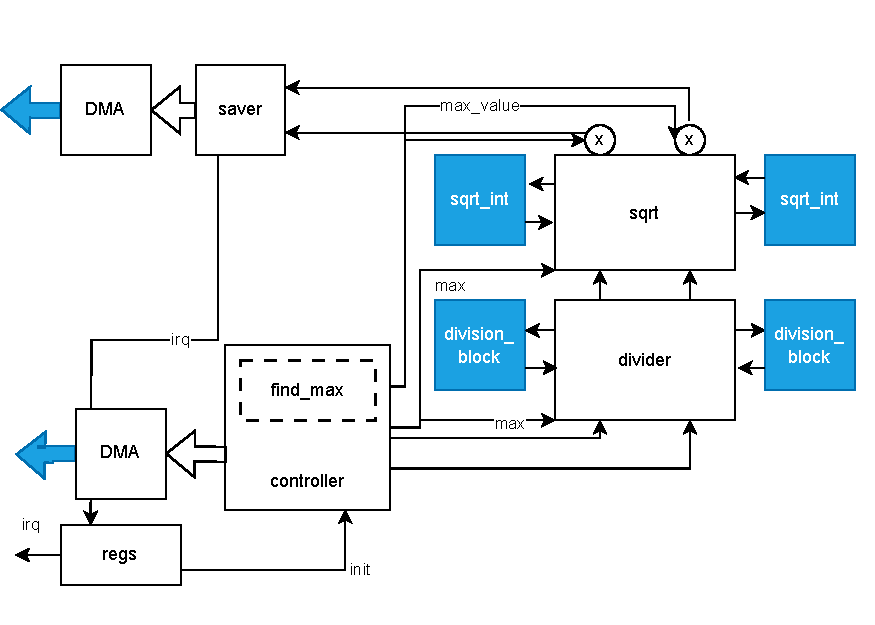
\includegraphics[width=1\textwidth]{Normalizer.pdf}
	\caption{Schemat komponentu \textit{Normalizer}}
\end{figure}
\FloatBarrier %zatrzymanie przenoszenia rysunku

\subsubsection{Kontroler}
Automat stanów \textbf{controller} opisany jest na rys. 4.26. Moduł zgodnie z~poprzednim rozdziałem realizuje 2 cykle ładowań danych za pośrednictwem \textit{DMA}. Do tego celu wykorzystuje się ustawione wcześniej przez program za pomocą rejestrów adres początkowy i~końcowy. Komponent normalizuje tylko pierwszą strefę załadowanej linijki profilu (pojęcie stref wyjaśniono w~rozdziale 4.7). Moduł korzysta z~parametrów \textit{area1} i~\textit{area2}. Jeżeli licznik pobranych próbek wykryje, że przekroczono rozmiar \textit{area1}, wówczas adres zamiast dodawania 4, aby pobrać kolejną wartość 32-bitową, dodaje \textit{area2}. Pozwala to pominąć obszar, który nie ma być normalizowany. Na przykładzie profilu dźwięku będzie to obszar związany ze współczynnikiem \textit{ZCR}. Podobny zabieg zastosowano w~module \textit{saver}.

\begin{figure}[h]
	\centering
	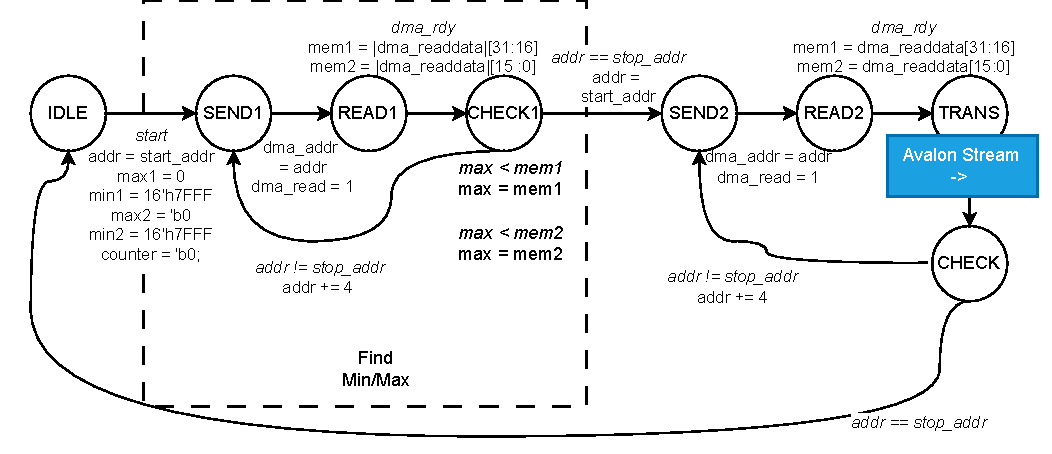
\includegraphics[width=1\textwidth]{Nor_Controller.pdf}
	\caption{Schemat automatu \textit{controller}}
\end{figure}
\FloatBarrier %zatrzymanie przenoszenia rysunku

\subsubsection{Rdzeń modułu}

Moduł \textbf{division} po otrzymaniu 16-bitowej wartości od modułu \textit{controller} separuje znak oraz wartość bezwzględną. Otrzymany moduł liczby oraz maksimum są przesuwane o~16 bitów w~lewo, aby móc realizować obliczenia w~notacji \textit{fixed point}. Liczby te przesyła się do modułów \textit{division\_block}, aby podzielić je tak jak liczby stałoprzecinkowe. Komponent realizuje algorytm dzielenia \cite{Division} z~modyfikacją pod kątem obsługi liczb \textit{fixed point}. Na interfejs wyjściowy wystawiane są najmłodsze 16 bitów, aby przesłać dalej jedynie część wartości odpowiedzialną za przechowywanie ułamkowej części liczby wraz ze znakiem.

Moduł \textbf{sqrt} otrzymuje wartości po interfejsie strumieniowym i~następnie realizuje koncepcję opisaną w~rozdziale 4.8. Zgodnie z~parametrem \textit{log\_nor} otrzymana wartość jest pierwiastkowana z~użyciem zewnętrznego modułu lub mnożona przez maksimum będące liczbą całkowitą. Po uzyskaniu wyniku mnożenia wystawia się do bloku \textit{saver} najstarsze 16 bitów z~32-bitowej wartości (co wynika z~mnożenia liczby całkowitej przez wartość o~precyzji 16 bitów po przecinku), zaś w~przypadku pierwiastkowania najmłodsze 16 bitów. Nie ma potrzeby zamiany liczby \textit{fixed point} na całkowitą, gdyż wybranie części ułamkowej z~wartości stałoprzecinkowej wyniku dzielenia przez maksimum daje znormalizowaną liczbę w~zakresie 0 - 65535. Po spierwiastkowaniu uzyskano wynik znormalizowany w~zakresie 0-255, który można swobodnie wystawić jako wartość finalną normalizacji pseudo-logarytmicznej.

Wynik jest zapisywany przez moduł \textbf{saver}, nadpisując blok opisany w~rejestrach konfiguracyjnych (adres początkowy i~końcowy). Stosuje się podobnie jak w~module \textit{loader} strefy, aby uniknąć niespójności danych, w~sposób podobny jak dla rozdziału 4.8.1. Różnica polega na tym, że zamiast operacji odczytu zastosowano operacje zapisu. Po zakończeniu działania moduł wysyła prośbę o~wystawienie przerwania do modułu rejestrów.

\subsubsection{Rejestry sterujące}

Komponent otrzymał offset 0x25000 oraz przerwanie o~numerze 4. Wymienione wcześniej rejestry są jedynie do zapisu, a~komponent informuje o~zakończeniu operacji przerwaniem. Układ rejestrów znajduje się na rys. 4.26. Na wyjściu wystawiane są najstarsze 16 bitów wyniku mnożenia liczby.

\begin{figure}[h]
	\centering
	\begin{tabular}{|r|r|r|}
		\hline
		Adres & Funkcja & Zakresy wartości\\
		\hline
		0x0 & Zwolnienie przerwania & Nadpisanie jakąkolwiek wartością \\
			&						& tego adresu powoduje \\
			&						& wyzerowanie przerwania procesorowego\\
		
		\hline 
		0x4 & Maksymalna wartość  & [15:0] (parametr \textit{max\_value})\\
		&   bezwzględna                  & \\
		
		\hline 
		0x8 & Adres początkowy & [31:0] (parametr \textit{start\_addr})\\
		
		\hline 
		0xc & Adres końcowy & [31:0] (parametr \textit{stop\_addr})\\
		\hline
		0x10 & Inicjacja operacji &Nadpisanie jakąkolwiek wartością tego adresu\\
		&& powoduje rozpoczęcie generowania profilu \\
		\hline
		0x14 &  Skalowanie logarytmiczne & [0] - 1'b1 skalowanie ,,logarytmiczne''\\
			 & 							 & 1'b0 - skalowanie liniowe \\
			 &							 & parametr \textit{log\_nor} \\
		
		\hline 
		0x18 & Strefy & [15:0] - rozmiar strefy 1 \textit{area1}\\
		     &        & [31:16] - rozmiar strefy 2 \textit{area2}\\
		\hline 
	\end{tabular}
	
	\caption{Rejestry komponentu \textit{Normalizer}}
\end{figure}
\FloatBarrier %zatrzymanie przenoszenia rysunku
\newpage
\section{Implementacja SoC}
\subsection{Koncepcja SoC}
Po opracowaniu komponentów odpowiedzialnych za detekcję słów, należało stworzyć pozostałą część systemu odpowiedzialną przede wszystkim za komunikację ze światem zewnętrznym. Należało stworzyć komponenty do odbioru dźwięku z~otoczenia, odtwarzania nagrań, odczytu zewnętrznych nośników na potrzeby komparatora. Dodatkowo należało opracować interakcję z~użytkownikiem poprzez przyciski (przykładowo, aby zresetować system), sposób informowania użytkownika o~stanie urządzenia oraz pomiar odległości pomiędzy użytkownikiem a~urządzeniem zgodnie z~ustaleniami w~ostatnim akapicie 3.3.1. Finalnie należało opracować komponent pozwalający na komunikację z~wykorzystaniem protokołu \textit{Bluetooth Low Energy}. Schemat wspominanego systemu znajduje się na rys. 5.1.

\begin{figure}[h]
	\centering
	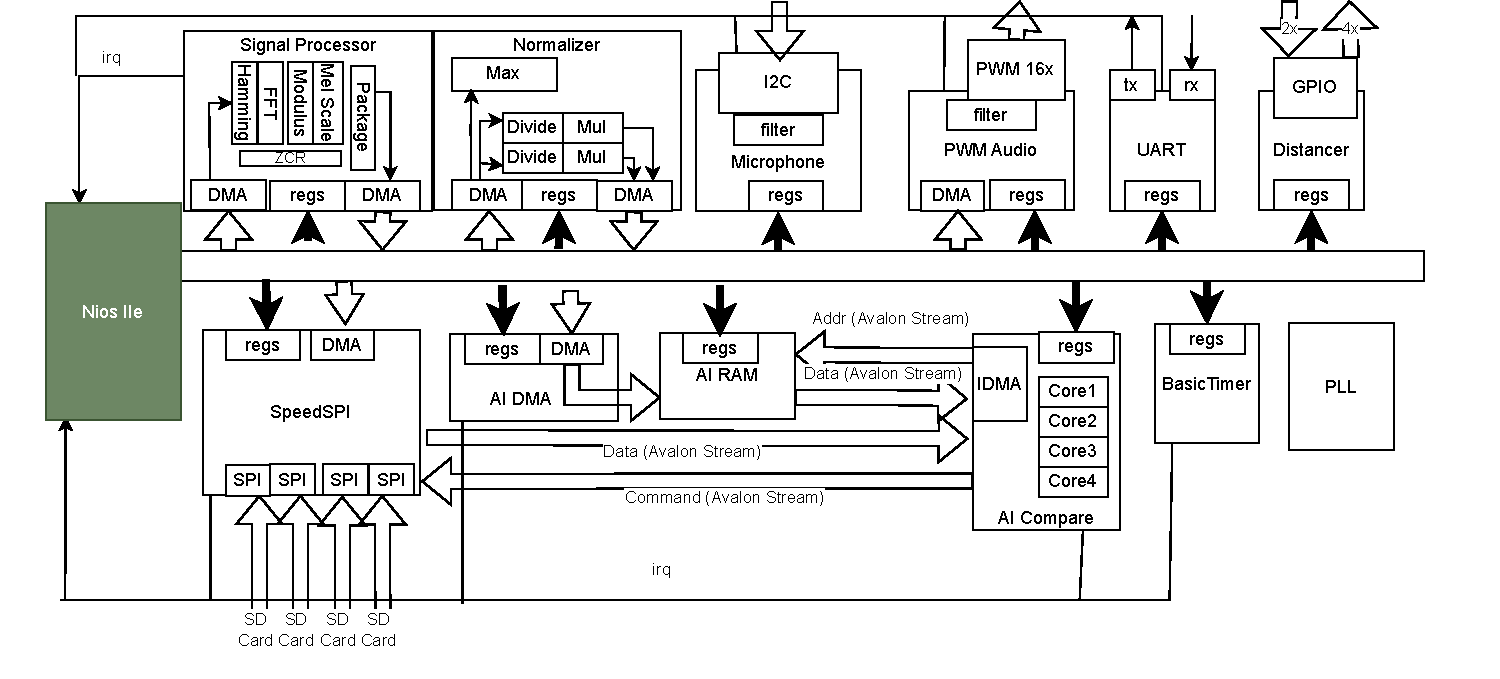
\includegraphics[width=1\textwidth]{all_system.pdf}
	\caption{Schemat systemu}
\end{figure}
\FloatBarrier

System, poza komponentami wcześniej opisanymi, składał się z~\textit{SpeedSPI}, \textit{Microphone}, \textit{PWM Audio}, \textit{UART}, \textit{Distancer} (GPIO) oraz timera \textit{BasicTimer}.

\textbf{SpeedSPI} umożliwia odczyt danych z~kart SD. Na potrzeby klasyfikatora potrafi on czytać 4 karty na raz, ponadto pozwala na odczyt danych z~pierwszego nośnika i~zapis za pomocą \textit{DMA} do pamięci. Pozwala to na odczyt zawartości nośnika przez program na potrzeby np. odtwarzania dźwięku czy obsługi systemu plików (rozdział 3.5). Do czytania danych z~kart komponent używa interfejsów SPI.

System pozwala na odbiór dźwięku przez mikrofon. Na potrzeby realizacji tego zadania opracowano komponent \textbf{Microphone}. Dzięki niemu system może odbierać próbki dźwięku, które mogą być zapisane przez procesor na potrzeby dalszego przetwarzania sygnałów. Odbiera on wartości za pomocą interfejsu I$^2$S, po czym przechodzą one przez odpowiedni filtr cyfrowy. Następnie trafiają do kolejki, z~której program może odczytywać potrzebne dane.

Aby odtwarzać dźwięki, opracowano komponent \textbf{PWM\_Audio}. Pozwala on, aby odczytane przy użyciu \textit{DMA} nagranie mogło być odtworzone przy użyciu głośnika. Odebrane próbki są filtrowane, po czym imitowany jest sygnał analogowy za pomocą \textit{PWM}. Aby dźwięki były głośniejsze, zdecydowano się na wyprowadzenie aż 16 wyjść PWM, które podłączone są do dwóch głośników. Dźwięk wydawany przez głośniki jest monofoniczny.

Kolejnym komponentem jest \textbf{BLE\_UART}, pozwalający na komunikację z~płytką obsługującą interfejs \textit{BLE}. Dzięki niemu urządzenie może wysyłać informacje dalej w~celu dalszego przetworzenia przez większy system. Dodatkowo, na potrzeby obsługi przycisków i~prostych komunikatów, w~systemie znajduje się komponent \textbf{GPIO}, który pozwala na obsługę diod przekazujących informację o~stanie urządzenia, komponentu mierzącego odległość pomiędzy użytkownikiem a~urządzeniem oraz przycisków. System, aby mógł dokonywać pomiarów czasu na potrzeby programu, korzysta z~uproszczonej wersji timera wystawiającego przerwanie co określony okres czasu.

Płytka DE10-Lite ma zegar 50 MHz. Aby przyspieszyć system, zdecydowano się na zwiększenie jego częstotliwości do 100 MHz za pomocą pętli sprzężenia fazowego. Zegar jest mnożony 2 razy. Do tego celu wykorzystano dostarczony przez producenta układu FPGA IP Core \textit{ALTPLL Intel FPGA IP}, za pomocą którego doprowadzono nowy zegar do wszystkich komponentów systemu, jak pokazano w~załączniku 1.

\subsection{Dobór komponentów zewnętrznych}

Po ustaleniu interfejsów, jakich komponenty używają do komunikacji z~systemem, dobrano odpowiednie czujniki zewnętrzne do odbierania danych z~otoczenia. Jako moduł komunikacyjny BLE system stosuje płytkę \textit{HM10} \cite{HM10} używaną w~trybie master, pozwalającą na odbieranie danych. Skonfigurowana jest tak, aby komunikowała się z~systemem poprzez interfejs UART o~prędkości 115200 baud.

Jako mikrofon system używa mikrofonu MEMS \textit{MSM261S4030H0R} \cite{Microphone}. Próbki podczas komunikacji po I$^2$S \cite{Wiki
} są odbierane tylko przez jeden kanał, dlatego dźwięk jest monofoniczny (tak jak dźwięki w~modelu). Do wydawania dźwięków używa się dwóch głośników YD30 0,5 W~o~impedancji 8 Ohm.

System stosuje również dwa przyciski pojemnościowe \cite{Button}: jeden do zmiany głośności, a~drugi, w~zależności od czasu przytrzymania przycisku, albo do resetu urządzenia, albo do rozpoczęcia nasłuchu rozkazów bez wywoływania imienia. Do komunikowania stanu urządzenia użyto 4 diod - 3 czerwonych i~jednej zielonej. Przyciski, jak i~diody, są podłączone do GPIO.

Jako czujnik odległości, który podłączony jest do modułu \textit{Distancer}, użyto ultradźwiękowego detektora \textit{HC-SR04} \cite{Distance}, pozwalającego na pomiar odległości w~przedziale 2-200 cm. W~prototypie stosuje się karty SD o~pojemności do 64 GB różnych producentów (ScanDisk, Kingston, Goodram).

Aby podłączyć karty SD do płytki w~systemie, stosuje się odpowiedni moduł czytnika \cite{Shield} od firmy Waveshare. Użyto 4 takie komponenty. Do przechowywania danych zastosowano karty, które umożliwiają komunikację po interfejsie \textit{SPI} o~częstotliwości zegara wynoszącej 50 - 67 MHz.

Aby podłączyć wcześniej wspomniane komponenty, używa się pinów GPIO oraz tych związanych z~wyjściami \textit{Arduino}, zgodnie z~dokumentacją płytki z~układem FPGA \cite{DE10L}.

\subsection{Komponent \textit{SpeedSPI}}
\subsubsection{Architektura komponentu}
Komponent \textbf{SpeedSPI} umożliwia jednoczesny odczyt danych z~4 kart SD na potrzeby klasyfikatora oraz z~jednej karty w~dedykowanym wyjściu na potrzeby programu procesora. Schemat budowy tego komponentu przedstawiono na rysunku 5.2.

\begin{figure}[h]
	\centering
	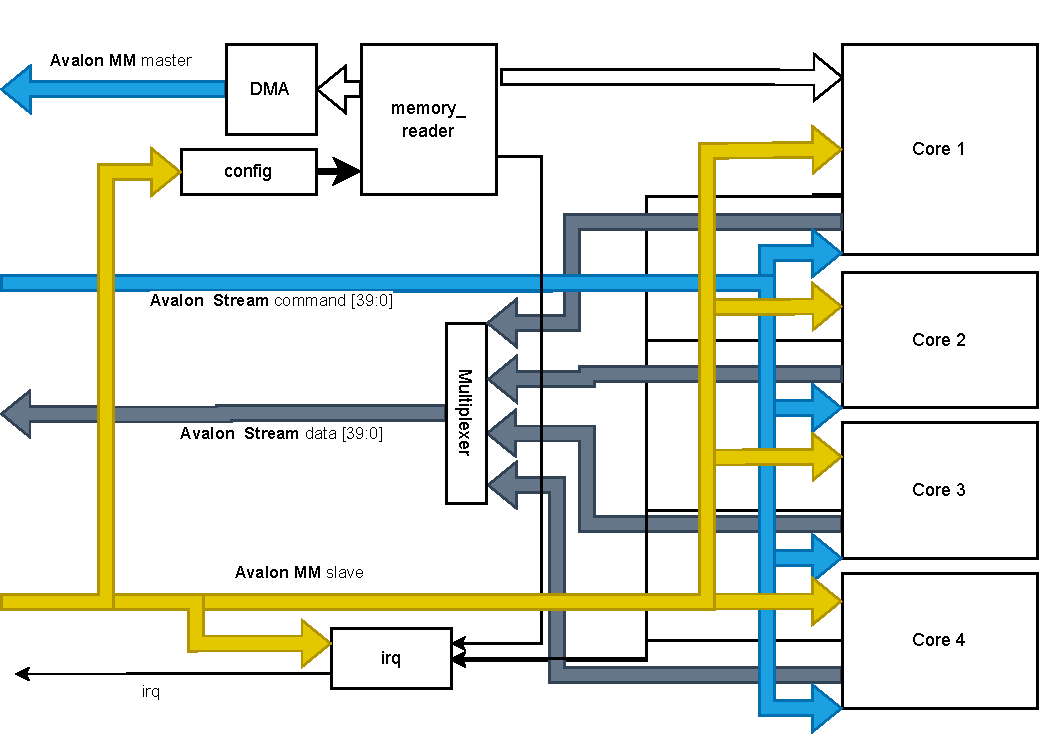
\includegraphics[width=1\textwidth]{SpeedSPI.pdf}
	\caption{Schemat architektury komponentu \textit{SpeedSPI}}
\end{figure}
\FloatBarrier %zatrzymanie przenoszenia rysunku

Komponent składa się z~4 rdzeni (\textit{core}), z~których każdy odpowiada za odczyt danych z~jednej karty. Rdzeń jest podłączony do interfejsów strumieniowych \textit{Avalon Stream}. Interfejs wejściowy \textit{command} pochodzi bezpośrednio z~komponentu \textit{AI\_comparer}, który przesyła polecenie równoległego odczytu danych z~4 kart SD. Interfejs ten jest podłączony do każdego rdzenia bez pośredniczenia przez specjalny moduł, a~cały komponent wystawia sygnał \textit{ready} w~stanie wysokim, co pozwala na uzyskanie prostego połączenia dla wielu wejść interfejsu strumieniowego.

Kolejnym interfejsem strumieniowym używanym przez rdzeń jest 8-bitowy interfejs wyjściowy \textit{data\_core}, za pomocą którego rdzeń transmituje odczytane dane z~karty SD opatrzone odpowiednim nagłówkiem (zgodnie z~założeniami z~rozdziału 4.5.5). Dane te są łączone w~formę pakietu przez moduł \textbf{Multiplexer}. Budowę niego określono w~rozdziale 4.5.2, po czym są one przesyłane do komponentu \textit{AI\_Comparer} przez 40-bitowy interfejs \textit{data}.

Każdy rdzeń ma również dostęp do interfejsu \textit{Avalon Memory Mapped}, który jest udostępniony do szyny procesora. Pozwala to na inicjację karty SD (każda karta SD wymaga przed odczytem lub zapisem danych wykonania procedury określonej w~specyfikacji standardu kart SD \cite{SDA}) z~poziomu programu procesora.

Moduł \textbf{irq} zbiera przerwania z~rdzeni, które są przekazywane do procesora i~mogą być zwolnione przez program dzięki podłączeniu go do interfejsu \textit{Avalon MM}, tego samego, do którego podłączono rdzenie kart \textit{SD}.

Jeden z~rdzeni posiada dodatkowe wyjście \textit{Avalon MM} do wewnętrznego sterowania daną kartą, co pozwala na wysyłanie sprecyzowanych danych poleceń nośnika. Automat \textbf{memory\_reader} wykonuje polecenie \textit{CMD17} (odczyt strumieniowy z~danego sektora \cite{SDA}), które jest wykonywane na podstawie parametrów ustawianych w~komponencie \textbf{config}. Dane są zapisywane pod odpowiednim adresem pamięci procesora za pomocą standardowego dla tego projektu modułu \textit{DMA} (specyfikacja określona w~rozdziale 4.3).

\subsubsection{Budowa rdzenia \textit{SpeedSPI\_card\_core}}
Budowę rdzenia komponentu zaprezentowano na rysunku 5.3. Moduł odpowiada za transakcje po interfejsie \textit{SPI} związane z~jedną kartą.

Modułami odpowiedzialnymi za bezpośrednią komunikację po interfejsie \textit{SPI} są \textit{read} i~\textit{send}. Moduł \textbf{read} pozwala na odbiór danych, zaś \textbf{send} na wysyłanie jednego bajta danych po wspomnianym interfejsie. Moduł \textit{read} kontroluje linię \textit{MISO}, a~\textit{send} linię \textit{MOSI}. Moduły te udostępniają także zegar interfejsu \textit{SCK}. Istnieje moduł korzystający z~logiki kombinacyjnej, wybierający zegar, który będzie wystawiany na wyjściu na podstawie sygnałów z~wspomnianych modułów.

Automat \textit{send} jest automatem stanów, który wysyła dane po interfejsie z~prędkością 50 MHz. Moduł \textit{read} czyta dane z~szybkością 50 MHz lub 66,7 MHz. Stworzono dwie wersje tego modułu: jedną, która korzysta z~automatu stanów w~tej samej domenie zegarowej co cały system (sterujący interfejsem z~częstotliwością 50 MHz) oraz drugą, pozwalającą na uzyskanie częstotliwości 66,7 MHz, która wymaga do prawidłowego działania oddzielnej domeny zegarowej o~częstotliwości 200 MHz udostępnianej przez globalny PLL użyty w~systemie. Wersja ta jest szybsza od 50 MHz-owej, ale nie zapewnia pełnego zabezpieczenia przed pojawieniem się metastabilności przez niestworzenie w~pełni poprawnego przejścia między domenami zegarowymi. Jest to wersja eksperymentalna, ale pozwala na demonstrację maksymalnych możliwości urządzenia - gdyż wąskim gardłem tego systemu nie są obliczenia sztucznej inteligencji, a~szybkość czytania danych. Jedna i~druga operacja nie mogą dziać się jednocześnie.

\begin{figure}[h]
	\centering
	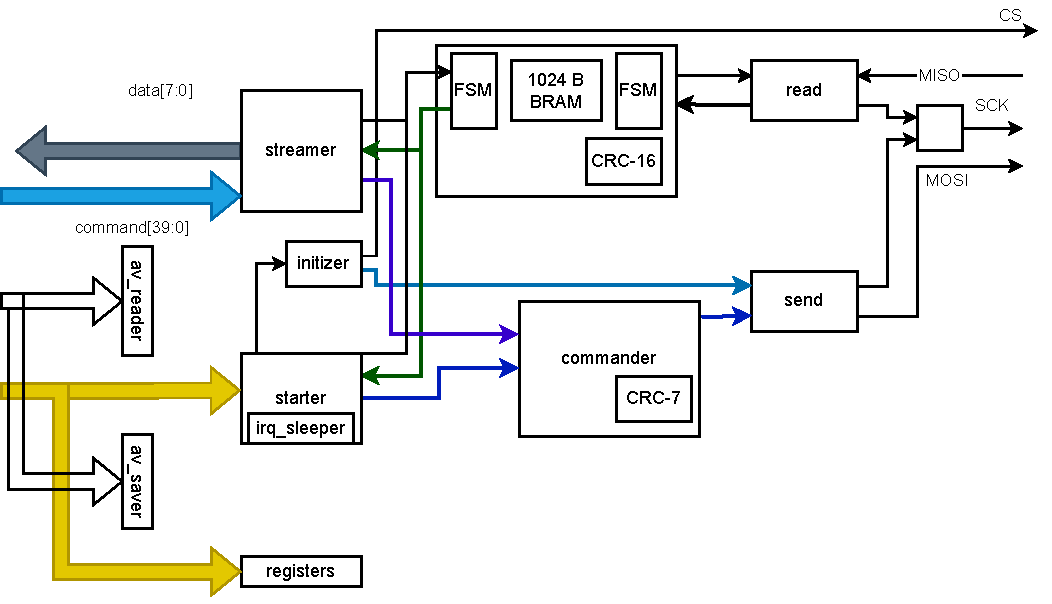
\includegraphics[width=1\textwidth]{SPICore.pdf}
	\caption{Schemat rdzenia dla odczytu jednej karty SD}
\end{figure}
\FloatBarrier %zatrzymanie przenoszenia rysunku

Linię \textit{CS} kontroluje moduł \textbf{initizer}. Linia ta jest w~stanie niskim (karta może przyjmować dane) przez cały czas poza procedurą wysłania 80 cykli rozruchowych wymaganych do uruchomienia karty SD (zgodnie ze standardem komunikacji z~kartą SD \cite{SDA}). Aby wysłać wspomniane cykle rozruchowe, wspomniany moduł podłączony jest do modułu \textit{send}, któremu zleca wysłanie 8 znaków 0xFF przy pinie \textit{CS} w~stanie wysokim.

Do modułu \textit{send} podłączony jest również \textbf{commander}. Pozwala on na wysłanie rozkazu do karty SD zgodnie z~formatem określonym w~specyfikacji \cite{SDA}. Na rysunku 5.4 znajduje się format takiej wiadomości.

\begin{figure}[h]
	\centering
	\begin{tabular}{|r|r|r|r|r|r|r|r|r|}
		\hline
		Wartość & 2'b01 & Numer komendy & Argument & CRC-7 & 1'b1 \\
		\hline
		Rozmiar & 2 bity & 6 bitów & 32 bitów & 7 bitów & 1 bit \\
		\hline
	\end{tabular}
	
	\caption{Blok danych wysyłany do karty SD wydania jej polecenia}
\end{figure}


Moduł \textbf{commander} odpowiada za przygotowanie polecenia w~formacie akceptowanym przez kartę SD. Składa się on z~automatu stanów, który generuje odpowiednią sekwencję bitów na podstawie parametrów ustawionych przez procesor. Komenda jest przesyłana przez interfejs \textit{SPI} za pośrednictwem modułu \textit{send}.

Dodatkowo, moduł \textit{read} obsługuje odbiór odpowiedzi z~karty SD po wysłaniu polecenia. Odbierane dane są przetwarzane przez moduł \textbf{responder}, który sprawdza poprawność odebranych danych i~zwraca je do procesora przez interfejs \textit{Avalon MM}.

Dzięki takiemu rozwiązaniu komponent \textbf{SpeedSPI} jest w~stanie efektywnie zarządzać komunikacją z~wieloma kartami SD jednocześnie, co znacząco przyspiesza proces odczytu danych niezbędnych do działania klasyfikatora.

Taka wiadomość, podzielona na bajty na podstawie żądań z~innych komponentów, jest wysyłana przez ten moduł. Moduł posiada wewnętrzną implementację obliczania odpowiedniego CRC-7, która jest podobna do tej zastosowanej w~komponencie \textit{AI\_Comparer} dla obliczania kontrolnego CRC-32 dla modelu. Ponieważ tylko \textit{initizer} i~\textit{commander} mają dostęp do wysyłania danych po interfejsie \textit{SPI}, nie ma możliwości zapisywania nowej zawartości na nośnikach.

Żądania odczytu danych trafiają jedynie z~modułu \textbf{loader}. Moduł ten odpowiada za buforowanie danych odebranych z~karty SD. Otrzymuje on żądanie załadowania sektora (standardowo dla kart SD 512 bajtów), po czym czyta dane z~karty. Sprawdza on jednocześnie integralność danych, weryfikując CRC-16 oraz czas odpowiedzi od karty.

Stan wspomnianych testów jest zapisywany w~buforze. Moduł pozwala w~czasie ładowania na odczyt zawartości przez inny moduł. Dzięki temu rdzeń może jednocześnie czytać dane z~sektora nośnika oraz wcześniej załadowane dane z~bufora, o~ile odczyt danych z~bufora jest szybszy od tego z~nośnika. Moduł zawiera wewnątrz siebie specjalną pamięć BRAM potrzebną do zapisywania odczytywanych danych z~nośnika. Umożliwia to ciągły odczyt danych wraz z~walidacją, zapobiegając nadpisaniu bloków pamięci nieodczytanych jeszcze przez rdzeń.

Dla standardu 66,7 MHz odczyt bajtu trwa 12 cykli zegarowych, zaś dla 50 MHz 16 cykli zegarowych. Dane z~bufora są czytane co 5 cykli, co spełnia założenia szybszego odczytu danych z~bufora niż ich ładowanie.

\textbf{Starter} odpowiada za inicjację karty zgodnie z~procedurą określoną w~specyfikacji standardu karty \textit{SD}, opisaną na schemacie 5.5.

\begin{figure}[h]
	\centering
	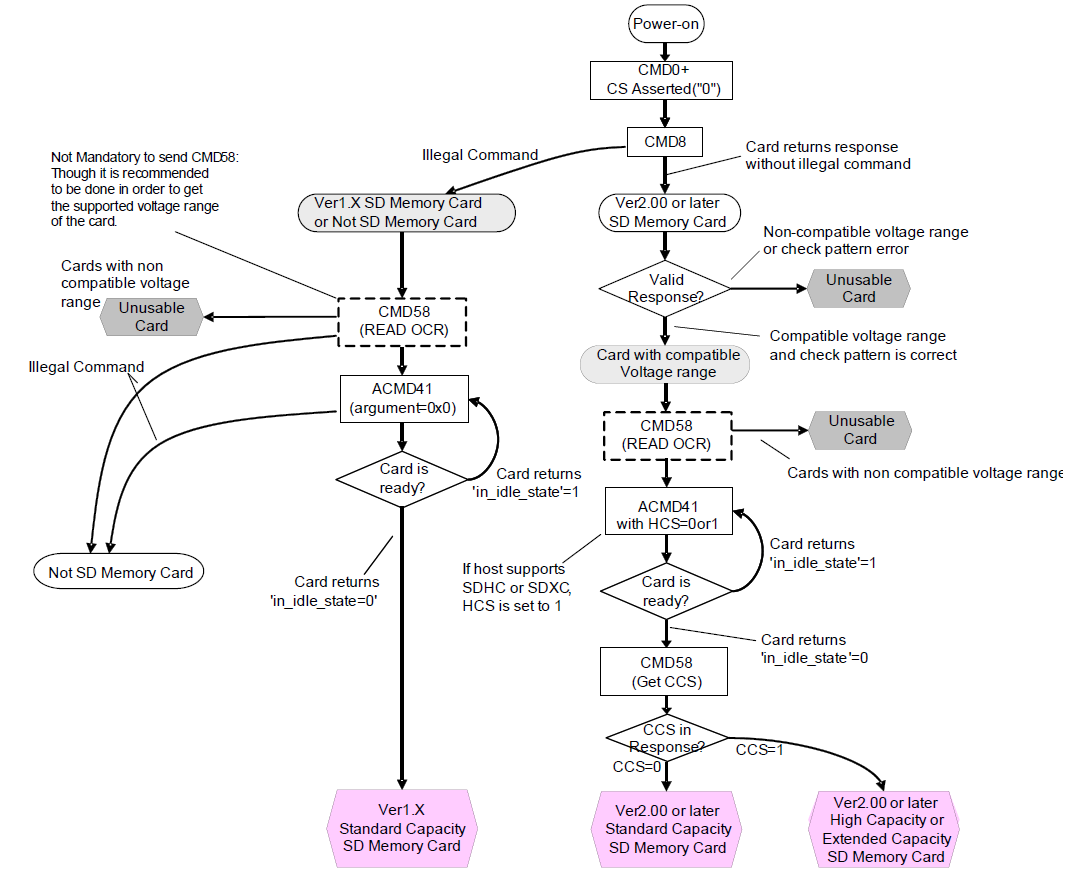
\includegraphics[width=1\textwidth]{init.png}
	\caption{Procedura inicjacji karty zgodnie z~specyfikacją \cite{SDA}}
\end{figure}
\FloatBarrier %zatrzymanie przenoszenia rysunku

Moduł \textbf{starter} rozpoczyna inicjację karty SD, wysyłając sekwencję odpowiednich poleceń przez interfejs \textit{SPI}. Proces ten obejmuje wysyłanie cykli synchronizacji, wysyłanie komendy resetującej (CMD0), a~następnie ustawienie napięcia operacyjnego i~trybu pracy karty. Wszystkie te operacje są zgodne ze specyfikacją standardu karty SD, zapewniając poprawną inicjalizację i~gotowość karty do odczytu i~zapisu danych.

Moduł \textbf{loader} po otrzymaniu żądania odczytu sektora, przechodzi do stanu odczytu, w~którym dane są pobierane z~karty i~zapisywane do wewnętrznej pamięci BRAM. Moduł sprawdza poprawność danych za pomocą weryfikacji CRC-16, a~w~przypadku wykrycia błędów, sygnalizuje je odpowiednimi flagami. Dzięki temu system jest w~stanie zapewnić wysoką integralność danych odczytywanych z~kart SD.

Kiedy dane są gotowe do odczytu przez rdzeń, moduł \textbf{loader} przełącza się w~tryb odczytu z~bufora, umożliwiając rdzeniowi dostęp do załadowanych danych z~minimalnym opóźnieniem. Dzięki zastosowaniu pamięci BRAM, system jest w~stanie zapewnić płynny przepływ danych, niezależnie od prędkości odczytu z~karty SD.

Na potrzeby systemu wykrycie karty o~wersji standardu rzędu 1.X jest uznawane za błąd. Moduł rozpoczyna pracę po nadpisaniu wartości udostępnionego rejestru oraz informuje o~zakończeniu operacji przerwaniem. Komendy muszą być wykonywane w~odpowiednim tempie – zbyt szybkie wywołanie nowego polecenia skutkowało podczas testów błędami. Aby temu zapobiec, wewnątrz modułu \textit{starter} znajduje się \textit{irq\_sleeper}, który opóźnia wewnętrzne przerwanie związane z~zakończeniem jednej z~operacji: wysłanie cyklów rozruchowych, zlecenie załadowania sektora do bufora, wysłanie rozkazu.

Zgodnie z~opisem z~rozdziału 5.3, jeden z~rdzeni ma wyprowadzony specjalny interfejs \textit{Avalon MM}, który pozwala na niskopoziomowe sterowanie rdzeniem. Używa go automat \textit{memory\_reader} do wykonywania swoich zadań na rdzeniu. Za tę komunikację odpowiadają moduły \textbf{av\_reader} i~\textbf{av\_writer}. Wykaz rejestrów udostępnionych przez interfejs \textit{Avalon MM}, którymi moduł \textit{memory\_reader} może sterować rdzeniem, znajduje się na rys. 5.6.

\begin{figure}[h]
	\centering
	\begin{tabular}{|r|r|r|}
		\hline
		Adres & Funkcja & Zakresy wartości\\
		\hline
		0x4 & Wysłanie komendy & [31:24] - kod komendy\\
			&				   & [23:0] - argument \\			
		0x8 & Odczyt bajtu z~bufora & [7:0] odczytany bajt\\			
		0xc & Zamknięcie karty SD & \\		
		0x10 & Inicjalizacja karty & \\
		0x14 & Załadowanie sektora & [31:0] długość ładowanych danych\\		
		\hline
	\end{tabular}
	
	\caption{Rejestry sterujące rdzeniem}
\end{figure}
\FloatBarrier %zatrzymanie przenoszenia rysunku



\subsubsection{Rejestry sterujące komponentem}


Komponent otrzymał offset 0x23000 oraz przerwanie o~numerze 2. Wymienione wcześniej rejestry są jedynie do zapisu, komponent informuje o~zakończeniu operacji przerwaniem. Układ rejestrów znajduje się na rys. 5.7.

\begin{figure}[h]
	\centering
	\begin{tabular}{|r|r|r|}
		\hline
		Adres & Funkcja & Zakresy wartości\\
		\hline
		0x0 & Zwolnienie przerwania & Nadpisanie jakąkolwiek wartością tego adresu\\
		&& powoduje wyzerowanie przerwania \\
	
		\hline 
		0x4 & Inicjacja rdzenia 1.  & Zapis jakiejkolwiek wartości \\
			&						& rozpoczyna procedurę inicjacji karty \\
			&						& Odczyt: \\
			&						& 32'h1 - prawidłowa inicjacja karty 	   \\
			&						& 32'h2 - brak odpowiedzi od karty		   		   \\
			&						& 32'h3 - Zbyt długie oczekiwanie na gotowość	   \\
			&						& karty										 	   \\
			&						& 32'h0 - nie inicjowano tej karty 	   			   \\
		\hline 
		0x8 & Inicjacja rdzenia 2.  & Analogicznie do rdzenia 1.\\
		\hline 		
		0xc & Inicjacja rdzenia 3.  & Analogicznie do rdzenia 1.\\
		\hline 						
		0x10 & Inicjacja rdzenia 4.  & Analogicznie do rdzenia 1.\\
		\hline 	
		
	\end{tabular}
\end{figure}
\begin{figure}[h]
	\begin{tabular}{|r|r|r|}
		\hline
		Adres & Funkcja & Zakresy wartości\\
		\hline
		0x14 & Adres początkowy do zapisu  & Tylko do zapisu [31:0] \\
			 & zawartości z~nośnika 1.	   &						\\
		\hline 	
		0x18 & Adres sektora oraz dlugość  & Tylko do zapisu [15:0] - \\
			 & odczytanego bloku danych	   & [31:16] - 				\\
		\hline
		0x1c & Rozpoczęcie odczytu		   & Zapis jakiejkolwiek wartości  \\
			 & zawartości z~nośnika 1.	   & rozpoczyna procedurę odczytu danych z~nośnika				\\
		\hline  				
	\end{tabular}
	
	\caption{Rejestry komponentu \textit{Speed\_SPI}}
\end{figure}
\FloatBarrier %zatrzymanie przenoszenia rysunku

\subsection{Komponent mikrofonu}
Komponent \textbf{Microphone} służy do odbioru sygnału dźwiękowego z~mikrofonu i~jego przetworzenia. Rysunek 5.8 prezentuje jego budowę.

\begin{figure}[h]
	\centering
	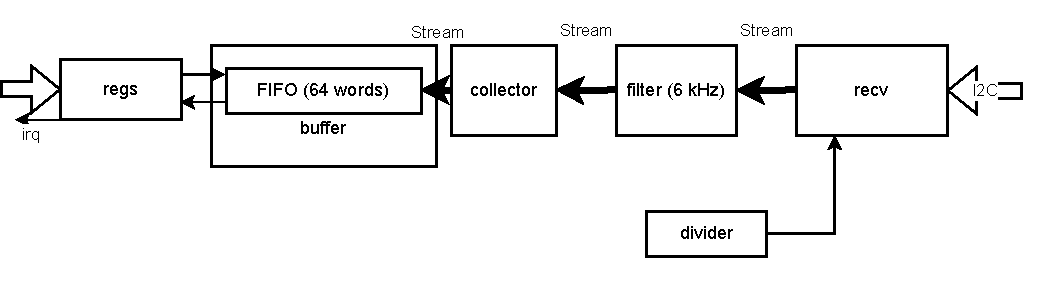
\includegraphics[width=1\textwidth]{Microphone.pdf}
	\caption{Schemat komponentu obsługującego mikrofon}
\end{figure}
\FloatBarrier %zatrzymanie przenoszenia rysunku

Komponent odbiera dane przy użyciu interfejsu \textit{I$^2$S}. Do tego celu wykorzystuje się moduł \textit{recv}, będący automatem stanów, który działa przez cały czas, zbierając 24-bitowe próbki 48 kHz-owego dźwięku z~kanału lewego. Format odbieranych danych prezentuje rys. 5.9.

Moduł udostępnia zegar (linia \textit{SCK}) interfejsowi oraz steruje linią \textit{WS} w~taki sposób, że dla kanału lewego jest ona w~stanie niskim, a~dla prawego w~stanie wysokim. Moduł nasłuchuje linii \textit{SD}, odczytując kolejno bity od 2 do 25, zbierając je w~interfejsie, co daje wartość 24-bitową. Dzięki temu uzyskuje się monofoniczny dźwięk. Interfejs I$^2$S działa z~częstotliwością 3,072 MHz. Odczytana wartość próbki jest wystawiana na interfejsie strumieniowym do filtra.

\begin{figure}[h]
	\centering
	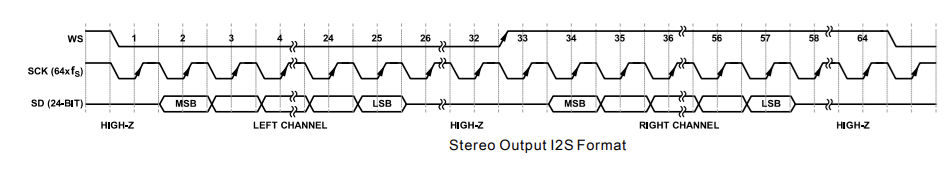
\includegraphics[width=1\textwidth]{I2C.png}
	\caption{Komunikacja z~mikrofonem po I$^2$S}
\end{figure}
\FloatBarrier %zatrzymanie przenoszenia rysunku

\textbf{Divider} jest modułem, który wysyła sygnał \textit{tick} co 16 lub 17 cykli zegarowych, aby uzyskać częstotliwość, której średnia wynosi żądaną wartość dla zastosowanego mikrofonu. Pozwala to na odmierzenie prawidłowych odstępów czasowych, tak aby w~odpowiednim tempie zmieniać stany na pinach wyjściowych interfejsu I$^2$S.

Moduł \textbf{filter} jest dolnoprzepustowym filtrem \textit{FIR} korzystającym z~własnej potokowej implementacji. Filtr ma 23 współczynniki i~działa zgodnie z~założeniami opisanymi w~rozdziale 2.1. Moduł zbiera opóźnione próbki, jednocześnie dokonując mnożeń z~współczynnikami filtra. Następnie potokowo zbierane są wyniki, które sumuje się. Proces sumowania podzielono na kilka etapów w~potoku, tworząc drzewo, co skróciło ścieżki krytyczne. Dzięki temu układ może działać z~szybszym zegarem. Finalnie, na wyjściu strumieniowym, takie jak dla \textit{recv}, wychodzą 24-bitowe próbki o~częstotliwości 48 kHz. Filtr ma częstotliwość graniczną 6 kHz oraz współczynniki pokazane na rys. 5.10. Takie podejście zapewnia, że przetworzone sygnały dźwiękowe są odpowiednio filtrowane, co umożliwia ich dalsze wykorzystanie w~systemie.

\begin{figure}[h]
\begin{lstlisting}[language=Python]
	
wspolczynniki = {
	-0,001107021588482344; 0,000146548252557626; 0,002354411824246723; 
	0,005206642050872691; 0,006392463561962282; 0.002348264305160368;
	-0.008704511540797525; -0.023246665480880974; -0.031476710933373515; 
	-0.020819573471449592; 0.017024975944599396; 0.079349116069050263;
	0.150569427091290925; 0.207406503294046751; 0.229112261242394033; 
	0.207406503294046751; 0.150569427091290925; 0.079349116069050277;
	0.017024975944599396; -0.020819573471449596; -0.031476710933373515; 
	-0.023246665480880981; -0.008704511540797533; 0.002348264305160369;
	0.006392463561962284; 0.005206642050872692; 0.002354411824246721;
	0.000146548252557627; -0.001107021588482344
}
	
\end{lstlisting}
\caption{Współczynniki filtru komponentu \textit{Microphone}}
\end{figure}
\FloatBarrier %zatrzymanie przenoszenia rysunku
Wartości zamieniono tak, aby były zgodne z~notacją \textit{fixed\_point} z~precyzją do 16 bitów po przecinku. Do wygenerowania tych współczynników wykorzystano narzędzie \textit{FIIR!} \cite{FIRDesign}.

Próbki trafiają z~filtra do bloku \textbf{collector}. W~nim odbywa się zmniejszenie częstotliwości próbkowania zgodnie z~założeniami z~rozdziału 3.2.1 (suma z~trzech próbek podzielona przez cztery). Powstałe w~ten sposób próbki odkłada się na kolejkę \textit{FIFO} o~rozmiarze 64 słów. Za pomocą rejestrów można pobierać dane z~tej kolejki. Aby kolejka przyjmowała dane, należy zainicjować komponent, nadpisując jeden z~rejestrów konfiguracyjnych.

Komponent otrzymał offset 0x28000 oraz numer przerwania 8. Podłączony jest do szyny procesora tak jak pozostałe komponenty przy użyciu narzędzia \textit{Platform Designer}. Rejestry konfiguracyjne są udostępnione do szyny adresowej poprzez interfejs \textit{Avalon MM}. Na rysunku 5.11 znajduje się spis rejestrów konfiguracyjnych wraz z~ich adresami. Wszystkie rejestry konfiguracyjne są w~trybie tylko do zapisu. Po skonfigurowaniu komponentu za pomocą tych rejestrów, procesor może pobierać próbki z~kolejki FIFO, inicjując odpowiednie operacje. Komponent informuje o~zakończeniu operacji za pomocą przerwania.



\begin{figure}[h]
	\centering
	\begin{tabular}{|r|r|r|}
		\hline
		Adres & Funkcja & Zakresy wartości\\
		\hline
		0x0 & Zwolnienie przerwania & Nadpisanie jakąkolwiek wartością tego adresu\\
		\hline 
		0x4 & Włączenie/ & Tylko do zapisu [0] rejestr \textit{enable} \\
			& Wyłącznie komponentu		 & 1'b1 - włączony 1'b0 - wyłącozny \\
		\hline
		0x8 & Odczyt wartości z~kolejki		 & Tylko do odczytu [23:0] - odczytana próbka\\
		\hline
		0xc & Stan kolejki					& Tylko do odczytu [1] - pełna kolejka\\
			&								& [0] - pusta kolejka\\

		\hline 
	\end{tabular}
	
	\caption{Rejestry komponentu \textit{Microphone}}
\end{figure}
\FloatBarrier %zatrzymanie przenoszenia rysunku

\subsection{Komponent modułu dźwiękowego \textit{PWM\_Audio}}
Komponent \textbf{PWM\_Audio} pozwala na odtwarzanie dźwięku monofonicznego o~częstotliwości próbkowania 48 kHz. Jego budowa jest zaprezentowana na rys. 5.12.

\begin{figure}[h]
	\centering
	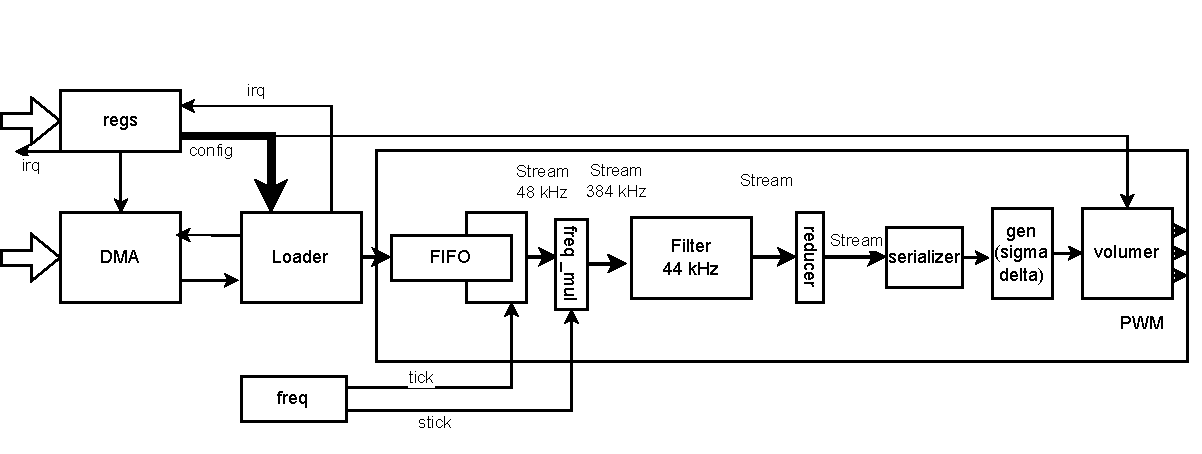
\includegraphics[width=1\textwidth]{PWM_Audio.pdf}
	\caption{Schemat komponentu odtwarzającego dźwięki}
\end{figure}
\FloatBarrier %zatrzymanie przenoszenia rysunku

Komponent ładuje dane za pomocą modułu \textbf{loader} przy użyciu standardowego \textit{DMA}, opisanego w~rozdziale 4.3. Moduł jest automatem stanów, który po inicjacji sygnałem \textit{init} pobiera po jednym słowie 32-bitowym, zaczynając od adresu określonego w~parametrze \textit{start\_addr}, po czym dzieli je na dwie wartości 16-bitowe. Najpierw wysyła interfejsem strumieniowym (składającym się z~sygnału 16-bitowego \textit{data} i~\textit{rdy}) wartość odczytaną z~bitów [15:0], a~później [31:16]. Proces jest zapętlony aż do odczytania adresu końcowego podanego w~parametrze \textit{stop\_addr}. Następnie moduł wysyła sygnał do modułu rejestrów (\textit{regs}), aby wystawił przerwanie do procesora i~wraca do stanu wyjściowego.

Kolejkę oraz moduły \textit{freq\_mul}, \textit{filter}, \textit{reducer} oraz \textit{serializer} połączono interfejsami strumieniowymi, podobnie jak w~module \textit{loader}.

Wartość wystawiana przez moduł \textit{loader} trafia do kolejki \textit{FIFO} (takiej samej jak dla mikrofonu). Moduł ten wystawia na wyjściowy interfejs dane z~odpowiednią częstotliwością zgodnie z~sygnałem \textit{tick}.

Dane z~kolejki trafiają do modułu \textbf{freq\_mul}, który mnoży częstotliwość wysyłanych próbek ośmiokrotnie. Zabieg ten pozwala na uzyskanie lepszego wygładzania sygnału przez filtr, co finalnie daje lepszą jakość dźwięku. Moduł po otrzymaniu próbki wystawia ją osiem razy na wyjściu w~tempie wyznaczanym przez sygnał \textit{stick}.

Sygnały \textit{stick} i~\textit{tick} są wysyłane przez moduł \textbf{freq}, który działa analogicznie do modułu \textit{divider} z~rozdziału 5.4. Wysyła on sygnał \textit{tick} co 2083 cykli zegarowych, co daje 48 kHz, oraz \textit{stick} co 260, co daje 384 kHz.

Próbki z~modułu \textit{freq\_mul} trafiają do filtra FIR dolnoprzepustowego o~częstotliwości granicznej 44 kHz. W~komponencie zastosowano tę samą implementację filtru co w~rozdziale 5.4, ale z~24 różnymi współczynnikami wymienionymi na rys. 5.13.

\begin{figure}[h]
\begin{lstlisting}[language=Python]
	
	wspolczynniki = {
	 -0,009516779255357086;-0,006634627097522952; -0,001964000252086015;
	  0,004526576810336817; 0,012717470176747183; 0,022333254551317520;
		0,032953052429183359; 0,044035716452676711; 0,054958065869915460;
		0,065062917629958472; 0,073712495949834603; 0,080342101272426983;
		0,084508760225141061; 0.085929990474856069; 0.084508760225141061;
		0.080342101272426983; 0.073712495949834603; 0.065062917629958472;
		0.054958065869915460; 0.044035716452676711; 0.032953052429183359;
		0.022333254551317520; 0.012717470176747183; 0.004526576810336817;
		-0.001964000252086015;-0.006634627097522952;-0.009516779255357086
	}
	
\end{lstlisting}
	\caption{Współczynniki filtru w~komponencie \textit{Audio\_PWM}}
\end{figure}
\FloatBarrier %zatrzymanie przenoszenia rysunku
Próbki z~filtru trafiają do modułu \textbf{reducer}, który dzieli je przez 2 (odpowiada za to przesunięcie bitowe), po czym trafiają do modułu \textbf{serializer}. Moduł zapisuje otrzymaną wartość do wewnętrznego rejestru, zamienia ją na wypełnienie sygnału dla generowanego dźwięku \textit{PWM} (negując najstarszy bit), a~następnie zatrzaskuje ją, wystawiając ją do generatora \textit{gen}.

Moduł \textbf{gen} jest pierwszorzędowym generatorem \textit{PWM} \cite{Wiki:PWM} sigma-delta \cite{Wiki:Sigma}. Do jego realizacji zastosowano zewnętrzną implementację \cite{SigmaDeltaI}, której kod głównego fragmentu generującego sygnał znajduje się na rys. 5.14.


\begin{figure}[h]
\begin{lstlisting}[language=Verilog]
	input [15:0] PWM_in;
	output PWM_out;
	
	reg [16:0] PWM_accumulator;
	always @(posedge clk) PWM_accumulator <= PWM_accumulator[15:0] 
+ PWM_in;
	
	assign PWM_out = PWM_accumulator[16];
\end{lstlisting}
	\caption{Kod generatora \textit{sigma-delta}}
\end{figure}
\FloatBarrier %zatrzymanie przenoszenia rysunku

Sygnał PWM trafia do modułu \textbf{volumer}. Tam sygnał jest mnożony na odpowiednią ilość wyjść z~komponentu, ustalonych przez parametr \textit{volume}.

Komponent otrzymał offset 0x26000 oraz numer przerwania 6. Jest podłączony do szyny procesora, tak jak pozostałe komponenty, za pomocą narzędzia \textit{Platform Designer}. Wspomniane wcześniej wartości parametrów są wystawiane z~modułu rejestrów. Rejestry konfiguracyjne są udostępnione do szyny adresowej poprzez interfejs \textit{Avalon MM}. Na rysunku 5.15 znajduje się spis rejestrów konfiguracyjnych wraz z~ich adresami.
 
 \begin{figure}[h]
 	\centering
 	\begin{tabular}{|r|r|r|}
 		\hline
 		Adres & Funkcja & Zakresy wartości\\
 		\hline
 		0x0 & Zwolnienie przerwania & Nadpisanie jakąkolwiek wartością tego adresu\\
 		\hline 
 		0x4 & Adres początkowy & Tylko do zapisu [31:0]  \\
 			&				   & parametr \textit{start\_addr} \\
 		\hline
 		0x8 & Adres końcowy	 & Tylko do zapisu [31:0] \\
 			&				 & parametr \textit{stop\_addr}\\
 		\hline
 		0xc & Poziom głośności	& Tylko do zapisu [3:0] \\
 			&				    & parametr \textit{volume}\\
 		
 		\hline 
  		0x10 & Inicjacja	 	& Nadpisanie jakąkolwiek wartością \\
 		   	 &- pełna kolejka    & powoduje inicjację modułu \textit{loader}\\		
 		\hline
 	\end{tabular}
 	
 	\caption{Rejestry komponentu \textit{Microphone}}
 \end{figure}
 \FloatBarrier %zatrzymanie przenoszenia rysunku
 
\subsection{Pozostałe komponenty}
W skład systemu wchodzą również mniejsze komponenty, takie jak \textit{Distancer}, \textit{BLE\_UART} oraz \textit{BasicTimer}.

Komponent \textit{Distancer} pełni rolę kontrolera GPIO, umożliwiając sterowanie 9 pinami wyjściowymi układu. Piny te są wykorzystywane do zapalania diod LED, co umożliwia użytkownikowi monitorowanie stanu urządzenia, oraz do obsługi układu mierzącego odległość. Procesor może sterować tymi pinami poprzez ustawienia rejestrów za pomocą interfejsu \textit{Avalon MM}. Dodatkowo, komponent \textit{Distancer} pozwala na odczyt stanów 3 pinów wejściowych: dwa z~nich są przeznaczone do obsługi przycisków, a~ostatni do odbioru sygnału z~układu pomiarowego. Komponent został przypisany do offsetu 0x27000.

Komponent \textit{BLE\_UART} odpowiada za komunikację poprzez interfejs UART, umożliwiając obsługę płytki \textit{HM10}, która realizuje komunikację Bluetooth Low Energy (BLE). Komponent posiada kolejkę wyjściową, zbierającą bajty do wysłania, oraz kolejkę wejściową, przechowującą odebrane bajty. Procesor może odczytywać pojedyncze bajty z~kolejki lub dodawać dane do wysłania poprzez odpowiednie rejestry konfiguracyjne. Komponent jest przystosowany do pracy z~prędkością 115200 baud. Ponadto, umożliwia monitorowanie stanu pinu \textit{STATE}, który sygnalizuje nawiązane połączenie BLE (stan wysoki). Każde odebranie lub wysłanie bajtu jest sygnalizowane przerwaniem o~numerze 7. Rejestry komponentu są dostępne przez interfejs \textit{Avalon MM}.

\textit{BasicTimer} to prosty timer generujący przerwanie w~ustalonych odstępach czasu, określonych w~cyklach zegarowych. Ustawienia te są konfigurowane poprzez rejestry dostępne za pośrednictwem interfejsu \textit{Avalon MM}. Komponent ma przypisany offset 0x22000 oraz numer przerwania 1. Timer ten może być używany do różnych zadań w~systemie, takich jak regularne sprawdzanie stanu komponentów, zarządzanie czasem próbkowania danych, czy realizacja zadań cyklicznych, które muszą być wykonywane w~określonych odstępach czasu.
 
Wyżej wspomniane komponenty podłączone są do szyny procesora za pomocą narzędzia \textit{Platform Designer}. Implementacja tych komponentów oraz ich integracja w~systemie pokazują kompleksowe podejście do tworzenia wszechstronnych i~skalowalnych rozwiązań embedded, które mogą być dostosowywane do różnych aplikacji poprzez odpowiednie modyfikacje konfiguracji i~parametrów systemowych.

\subsection{Podłączenie komponentów zewnętrznych}

Po stworzeniu projektu SoC, konieczne było podłączenie do układu FPGA zewnętrznych komponentów wymienionych w~rozdziale 5.2. Schemat podłączeń przedstawiono na rysunku 5.16.

Komponenty \textit{HC-SR04} oraz \textit{HM10} są zasilane napięciem 5~V, natomiast pozostałe elementy, w~tym karty SD i~diody, zasilane są napięciem 3,3~V. Diody są zabezpieczone przed przepływem zbyt dużego natężenia prądu poprzez dodanie szeregowo rezystorów o~wartości 1 k$\Omega$. Wyjścia PWM, generujące dźwięk, są podłączone do dwóch głośników. Połączenia związane z~jednym głośnikiem są złączone w~jeden węzeł, aby zgodnie z~prawem Kirchhoffa uzyskać odpowiednio duże natężenie prądu. Jest ono wprost proporcjonalne do liczby wyjść, na których generowany jest sygnał. Im większe natężenie prądu, tym głośniejszy dźwięk wydaje głośnik. Można było zastosować wzmacniacz, ale w~ramach budowy prototypu uznano, że takie rozwiązanie będzie prostsze w~implementacji.

\begin{figure}[h]
	\centering
	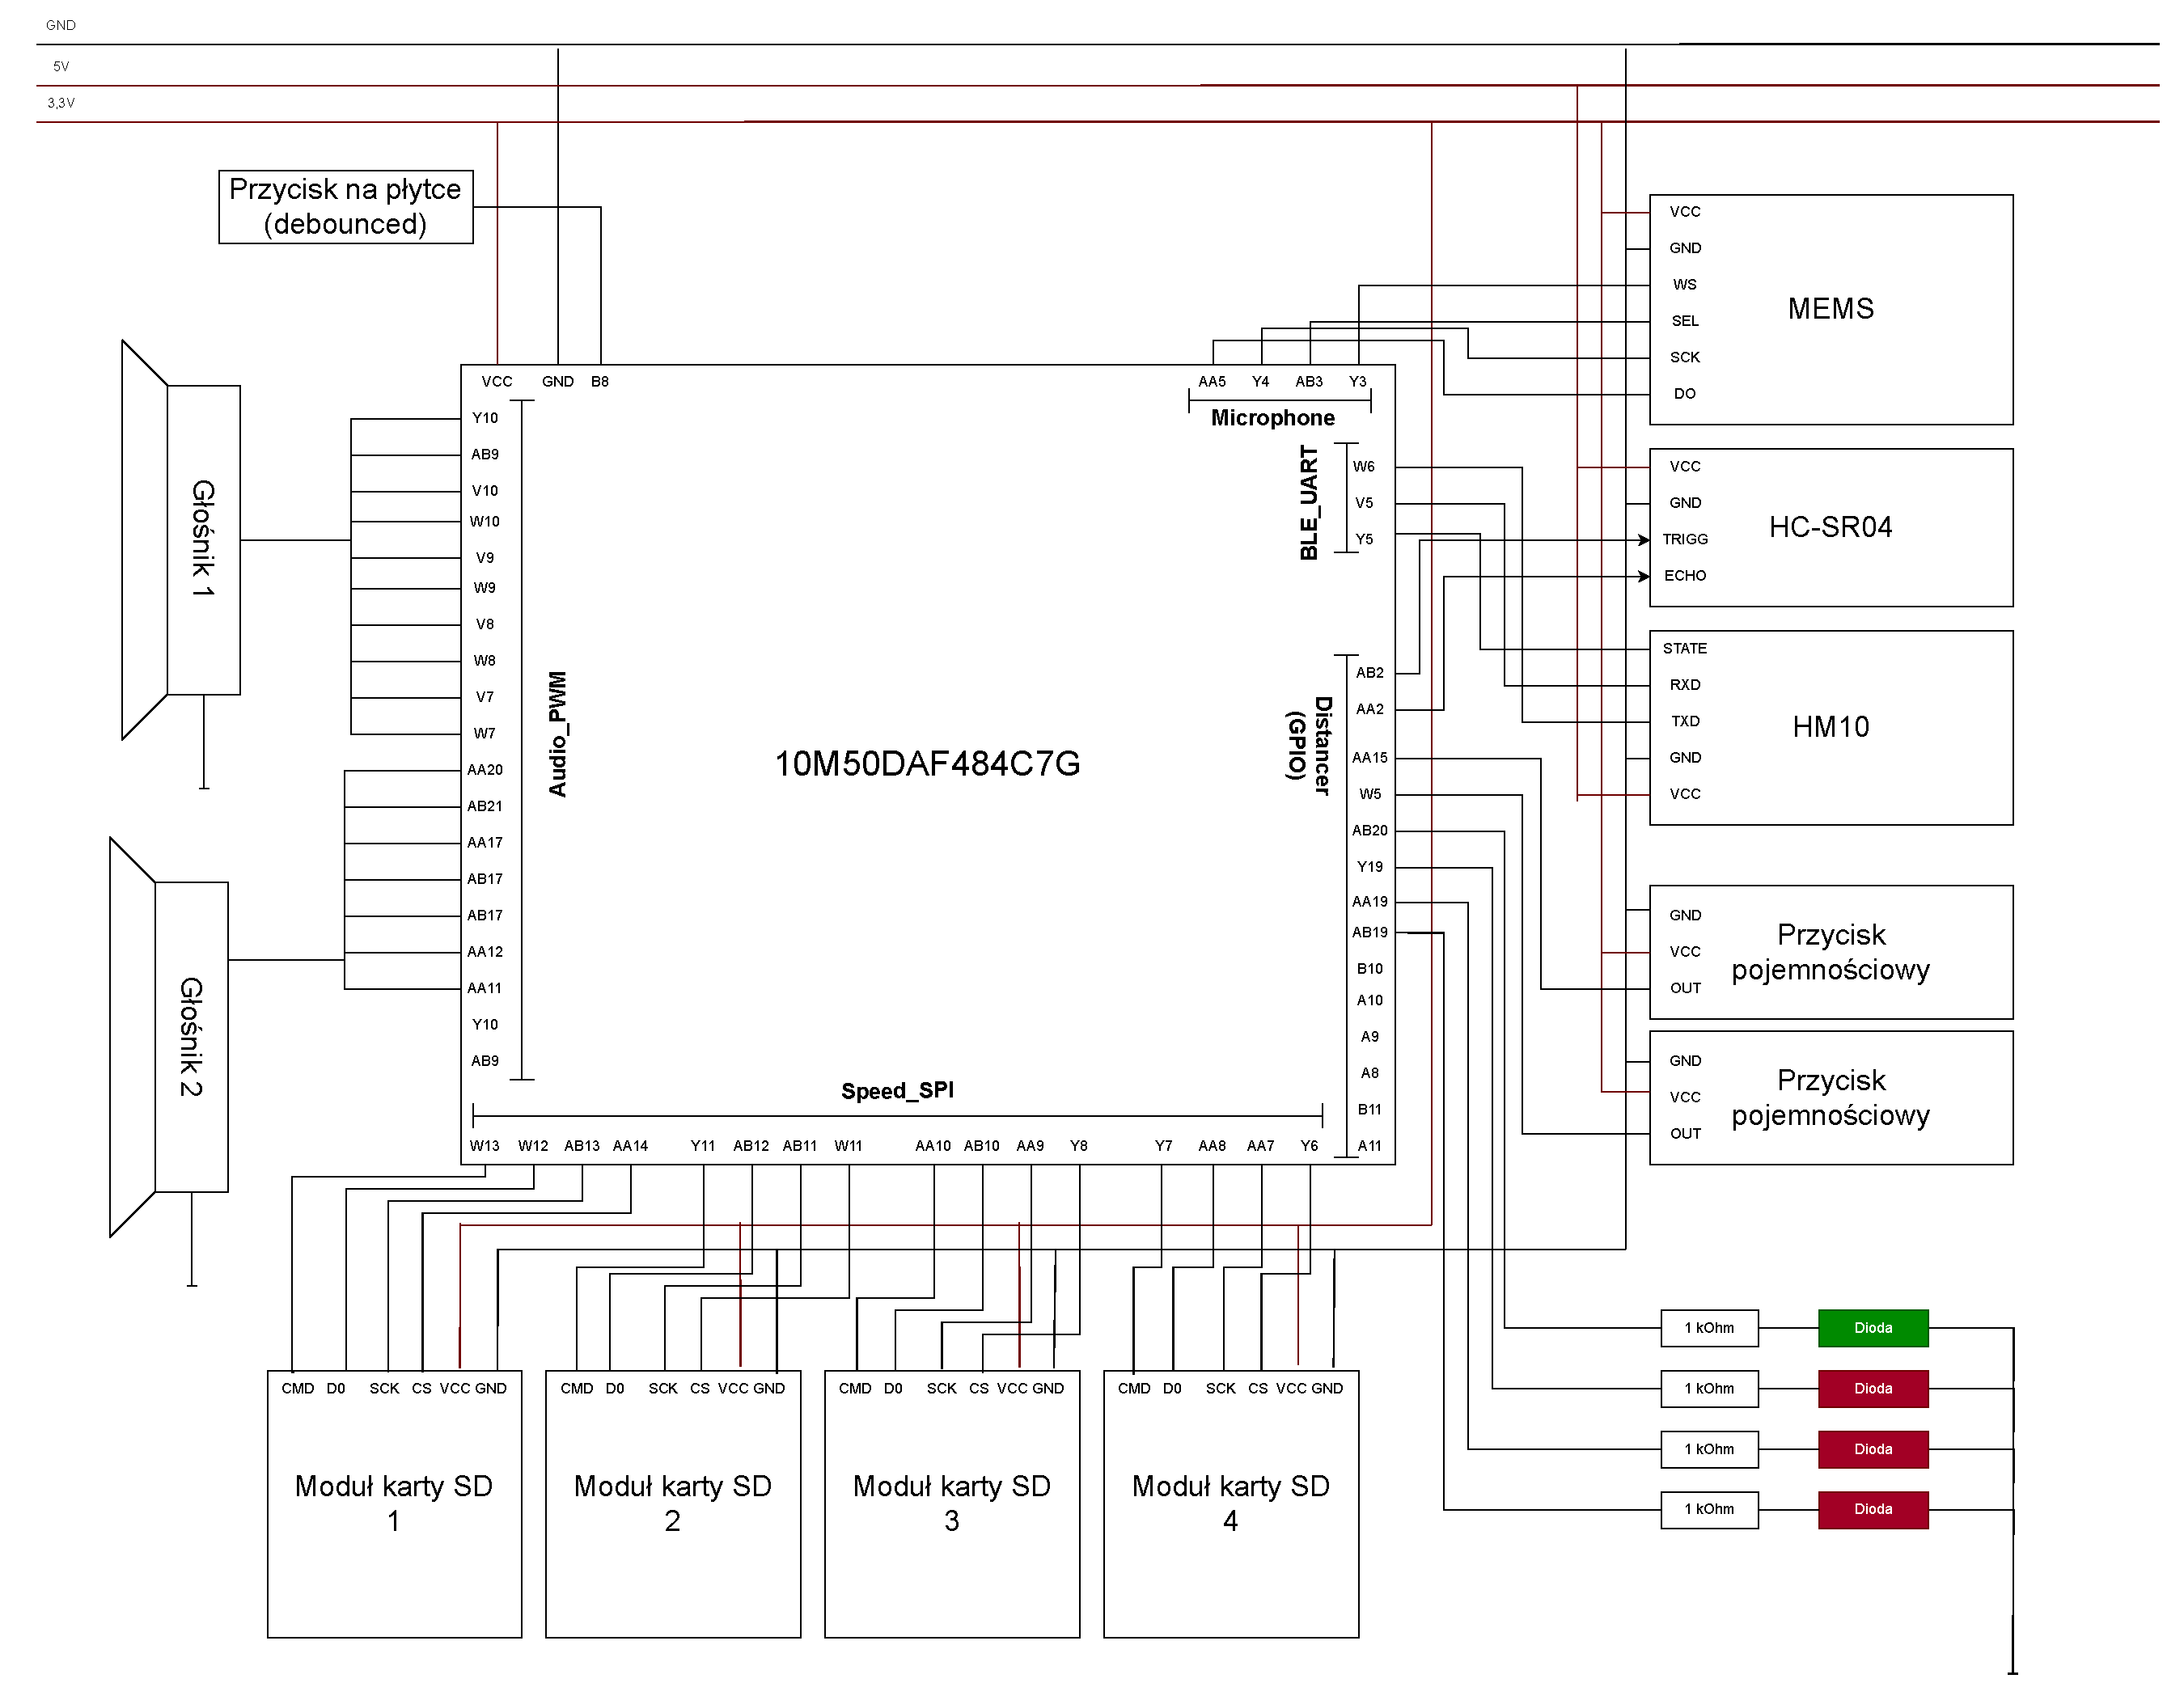
\includegraphics[width=1\textwidth]{Podlaczenie.pdf}
	\caption{Schemat podłączenia komponentów zewnętrznych do układu FPGA i~źródeł zasilania}
\end{figure}
\FloatBarrier %zatrzymanie przenoszenia rysunku

Ponieważ w~systemie zastosowano moduły gotowe, przystosowane do budowania prototypów, nie stosowano dodatkowych komponentów elektronicznych zabezpieczających układy zewnętrzne.

\subsubsection{Wyprowadzenia układu}

Wszystkim pinom wyjściowym i~wejściowym ustalono napięcie 3,3 V (standard wejścia-wyjścia \textit{LVTTL}) oraz natężenie 8 mA, poza tymi związanymi z~komunikacją dla JTAG-UART, gdzie ustalono napięcie 2,5 V oraz natężenie 12 mA, zgodnie z~sugestią narzędzia Pin Planner. Wykaz wyjść zaprezentowano na rys. 5.17.

Podczas nazywania wyjść związanych z~kartami SD, błędnie oznaczono wyjścia \textit{MISO} i~\textit{MOSI} – zamiast MOSI powinno być MISO i~vice versa.

\begin{figure}[h]
	\centering
	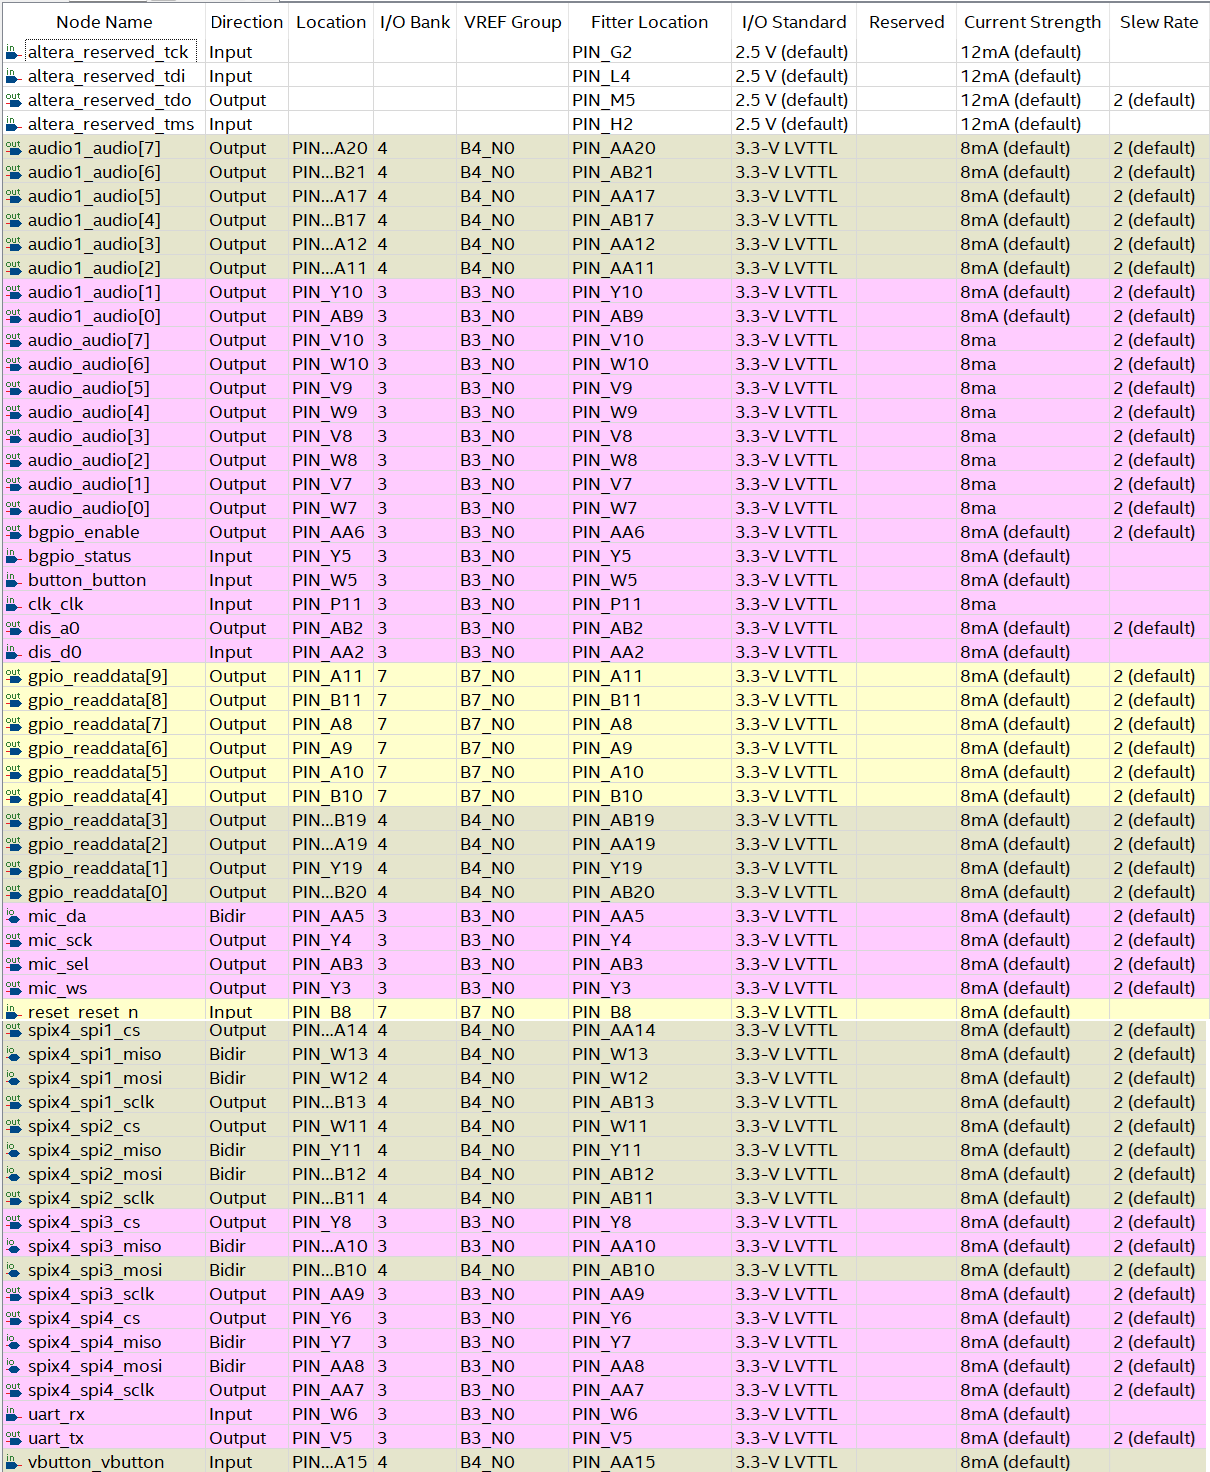
\includegraphics[width=1\textwidth]{Pinout.png}
	\caption{Wykaz wyprowadzeń dla projektu dla projektu}
\end{figure}
\FloatBarrier %zatrzymanie przenoszenia rysunku


\newpage
\section{Program urządzenia}
\subsection{Procedura wykrycia dźwięku}

Ostatnią częścią realizacji projektu w~ramach tej pracy było opracowanie oprogramowania dla użytego w~opracowanym SoC procesora NIOS II/e. Procesor w~wersji darmowej nie wspiera sprzętowego mnożenia, dzielenia oraz pamięci cache. Oznacza to, że pomimo taktowania tego procesora zegarem 100 MHz (tak jak cały system), program wykonywany na nim działałby stosunkowo wolno.

Mając na uwadze ograniczenia tej platformy, opracowano oprogramowanie, które pomimo tych ograniczeń działa na tyle efektywnie, aby proces wykrywania wyrazów nie był uciążliwy z~perspektywy użytkownika. Za umowną granicę komfortu uznano czas jednej sekundy. Oprogramowanie musiało zmieścić się w~pamięci RAM przydzielonej procesorowi, która wynosi 92 kB.

W docelowym rozwiązaniu zaprogramowano FPGA w~taki sposób, aby przy uruchomieniu układu (np. po otrzymaniu zasilania) załadował i~zbootował opracowane oprogramowanie. Do jego przechowywania użyto wbudowanej pamięci UFM.

Do opracowania oprogramowania użyto narzędzia \textit{NIOS II Software Build Tools for Eclipse}, które pozwala na stworzenie projektu oraz jego skompilowanie w~takiej formie, aby możliwe było jego nagranie na układ FPGA wraz z~implementacją sprzętową projektu.

\subsubsection{Nagrywanie dźwięku}

Procedura detekcji wyrazów rozpoczyna się od zbierania próbek przez bufor cykliczny zgodnie z~założeniami rozdziału 3.2.1. Po odebraniu przerwania z~mikrofonu program zwalnia przerwanie i~ustawia flagę dla pętli głównej nagrywającej dźwięk. Program po odebraniu flagi odczytuje z~odpowiedniego rejestru komponentu \textit{Microphone} i~sprawdza, czy kolejka nie jest przepełniona, korzystając z~rejestru komponentu. Wartość odebrana z~kolejki mikrofonu jest zamieniana z~wartości 24-bitowej na 16-bitową.

Gdy kolejka jest przepełniona, program czyści ją odpowiednią liczbą odczytów, po czym resetuje bufor cykliczny. Jeżeli kolejka nie jest przepełniona, odebrana próbka jest sprawdzana pod kątem poprawności. Jeżeli przez sekundę program odbiera próbki o~wartości 0xFFFF, oznacza to, że z~dużym prawdopodobieństwem na linii danych mikrofonu występuje wysoka impedancja. Może to oznaczać rozłączenie mikrofonu lub jego uszkodzenie. Komponent rejestruje próbki z~częstotliwością 16 kHz, co oznacza, że po odebraniu 16000 próbek o~wspomnianej wartości program zgłasza błąd krytyczny, który sygnalizuje miganiem jednej z~czerwonych diod na panelu.

Próbka uznana za prawidłową jest zapisywana do bufora cyklicznego o~rozmiarze 24000 próbek 16-bitowych. Jeżeli wykryta zostanie próbka o~wartości bezwzględnej większej niż 1536, wówczas ustawiany jest licznik \textit{margin} na 1 i~odliczane są kolejne próbki aż do 11950. Wówczas w~buforze zapisywane jest sąsiedztwo wykrytej \textit{głośnej} próbki: 0,75 sekundy nagrania przed nią i~0,75 sekundy po niej. Dzięki temu z~dużym prawdopodobieństwem taki zestaw danych zawiera całe słowo o~maksymalnie 2 sylabach.

Program, aby przechwytywać próbki, sprawdza też, czy użytkownik jest w~pobliżu, korzystając z~czujnika odległości. Do tego celu wykorzystywane jest przerwanie czasowe, które także odpowiada za miganie diodami. Program wystawia żądanie do przerwania czasowego za pomocą odpowiedniej struktury komunikacyjnej o~pomiar odległości. Przerwanie, otrzymując je, triggeruje czujnik, wystawiając stan wysoki na 1 ms na wyjście TRIGG. Wykorzystuje do tego rejestry komponentu \textit{Distancer}. Przerwanie sprawdza przy każdym wywołaniu (co 100 $\mu$s), czy najpierw występuje stan wysoki, a~potem niski. Gdy wystąpi wspomniana sekwencja, mierzony jest jej czas, który zwracany jest do programu przez wspomnianą strukturę. Sprawdzane są pewne warunki krytyczne, w~jakim momencie układ czujnika odpowiedział stanem wysokim. Jeżeli odbyło się to zbyt szybko, przekazywany jest błąd do programu głównego, a~ten zgłasza błąd krytyczny, sygnalizując to miganiem diody.

Zapisane w~buforze nagranie z~wykrytą \textit{głośną} próbką jest normalizowane liniowo za pomocą komponentu \textit{Normalizer} do maksymalnej wartości 512. Program, za pomocą rejestrów, wskazuje początek i~koniec bloku, w~którym zapisywano próbki z~mikrofonu, po czym inicjuje operację i~czeka na flagę przerwania od normalizatora.

Następnie próbki są kopiowane za pomocą \textit{AI\_DMA}, stosując przesunięcie do pamięci dedykowanej, aby uzyskać z~danych z~bufora cyklicznego uporządkowany zestaw próbek. Do tego celu przystosowano wspomniany komponent. Program konfiguruje go za pomocą udostępnionych rejestrów, wskazując adresy na podstawie wskaźników miejsc początku, końca bloku danych i~miejsca, gdzie zakończono zapisywanie próbek. Rejestr wag, w~przypadku kopiowania danych bez używania tej funkcjonalności, ustawiany jest na 0xFFFF. Następnie program czeka na przerwanie, po czym ponownie kopiuje dane bez użycia DMA do ich starego miejsca, stosując poniższy kod przedstawiony na rys. 6.1.


\begin{figure}[h]
\begin{lstlisting}[language=C]
	volatile uint16_t* table = memories -> table;
	volatile uint8_t* swap = memories -> swap;
	
	for(int k=0;k<len/2;k++){
		DMA_swap_mem_t get = swap[k];
		DMA_table_mem_t value = 0;
		
		if(get >> 7 == 0x1){
			value = ((get << 2) | 0x3) | MINUS_12_BITS;
		}else{
			value = get << 2;
		}
		
		table[k] = value;
	}
\end{lstlisting}
\caption{Kod funkcji kopiującej dane z~dedykowanej pamięci \textit{AI\_RAM}}
\end{figure}
\FloatBarrier %zatrzymanie przenoszenia rysunku

gdzie \textit{table} to pamięć, w~której zapisano dane z~mikrofonu, a~\textit{swap} to pamięć specjalna dla AI. W~ten sposób, używając małej ilości pamięci, porządkuje się dane z~bufora cyklicznego kosztem ich precyzji. Precyzja ta jest wystarczająca na potrzeby detekcji dla urządzenia embedded, a~zastosowanie komponentu sprzętowego znacznie przyspieszyło proces.

\subsubsection{Wybór \textit{głośnego} fragmentu}

Uporządkowane dane analizowane są w~celu wybrania głośnego fragmentu. Algorytm tego procesu opisano w~rozdziale 3.2.1. Wynikiem jest uzyskanie adresu początkowego i~końcowego fragmentu do dalszej analizy. Następnie ponownie kopiujemy dane przez \textit{AI\_DMA}, wskazując na wyznaczony blok danych oraz adres startowy na jego początek. Wówczas komponent nie porządkuje danych tak jak przy wcześniejszym kopiowaniu, a~jedynie kopiuje fragment do pamięci specjalnej. Tutaj również wykorzystuje się wbudowane w~komponent przesunięcie.

Dane wracają z~powrotem do tablicy z~próbkami, podobnie jak przy sortowaniu danych bufora cyklicznego. W~ten sposób wydziela się fragment nagrania, który potencjalnie może być wymawianym słowem. W~przypadku, gdy kod nie wykryje fragmentu spełniającego minimalne wymagania (określone w~rozdziale 3.2.1), program zwraca informację o~wykryciu szumu, po czym czyści tablicę bufora cyklicznego i~wraca do nagrywania dźwięków od nowa.

\subsubsection{Pomiar cech kluczowych}
Próbkom \textit{głośnego} fragmentu wyznacza się profile dla każdej 512-próbkowej ramki, po czym cały zestaw danych normalizowany jest logarytmicznie.

Najpierw pętla wyznacza adresy początku i~końca kolejnych ramek. Dla każdej iteracji komponent ustawia \textit{Signal\_Processor}, po czym czeka na przerwanie. Operację wykonuje się tyle razy, ile jest potrzebne do przeanalizowania wszystkich próbek.

Następnie program, przy użyciu komponentu \textit{Normalizer}, normalizuje cały analizowany zakres używając stref (zgodnie ze specyfikacją dla linijki o~320 próbkach: 1. strefa 256 próbek dla spektrogramu oraz 2. strefa 64 próbek dla ZCR) za pomocą sprzętowego normalizatora. Normalizuje się je w~taki sposób, aby normalizować tylko pierwszą strefę.

Po przygotowaniu profilu skaluje się go w~osi czasu, aby zawsze składał się z~64 linijek, bez względu na to, jak długi był przechwycony fragment. Do tego celu wykorzystuje się funkcję programu urządzenia, którego kod znajduje się na rys. 6.2.

\begin{figure}[h]
\begin{lstlisting}[language=C]
	
#define FIXED_POINT_POS 16
#define INT_TO_FIXED_POINT(n) (uint32_t) (n << (FIXED_POINT_POS - 1))
#define FIXED_TO_INT_POINT(n) (uint32_t) (n >> (FIXED_POINT_POS - 1))
typedef uint32_t fixed_t;
	
	...
	
	fixed_t delta =  INT_TO_FIXED_POINT(height)/ stoppos;
	fixed_t deltar = delta;
	
	for (uint32_t no =0 ; no < width; no++) {
		int offset = no;
		
		uint16_t old_border[height];
		uint16_t new_border[height];
		
		for (uint32_t n = 0; n < height; n++) {
			
			if (n < stoppos) {
				old_border[n] = table[offset];
				offset += width;
			} else {
				old_border[n] = 0;
			}
			
			new_border[n] = 0;
		}
		
		int posX = 0;
		for (uint32_t n = 0; n < stoppos; n++) {
			
			fixed_t startPos = posX;
			fixed_t stopPos = posX + deltar;
			
			for (uint32_t k = FIXED_TO_INT_POINT(startPos); k <
			FIXED_TO_INT_POINT(stopPos); k++) {
				
				if(k < height){
					if (new_border[k] < old_border[n])
					new_border[k] = old_border[n];
				}
			}
			
			
			posX += deltar;
		}
		
		offset = no;
		for (uint32_t n = 0; n < height; n++) {
			table[offset] = new_border[n];
			offset += width;
		}
	}
\end{lstlisting}
	\caption{Kod funkcji normalizującej w~dziedzinie czasu}
\end{figure}
\FloatBarrier %zatrzymanie przenoszenia rysunku


Zapisuje on do bufora z~każdej linijki profilu próbki o~tym samym numerze. Linijkę skaluje się metodą najbliższego sąsiada, korzystając z~algebry \textit{fixed\_point}. Następnie program zapisuje je, nadpisując kolejnymi linijkami profilu próbki o~danym numerze. Program analizuje w~ten sposób wszystkie 320 numery próbek dla linijki.

Tak uzyskany profil może być wykorzystany przez klasyfikator do porównania z~innymi profilami w~modelu. Model kopiowany jest za pomocą \textit{AI\_DMA}, z~uwzględnieniem stref oraz minimum dla strefy 1. (Aby usunąć z~profilu nieistotne informacje, zgodnie z~rozdziałem 3.2.2, należy usunąć próbki z~widma o~wartości poniżej 16). Program, po wykryciu flagi przerwania od \textit{AI\_DMA}, może przejść do klasyfikacji wychwyconego głośnego dźwięku, który może być wyrazem.

\subsubsection{Analiza modelu}

Program odczytuje z~pierwszej karty dane na temat modelu. Do tego celu używa komponentu \textit{SpeedSPI}. Program, przy użyciu wspomnianego modułu, odczytuje dane z~nośnika oraz interpretuje je zgodnie ze specyfikacją systemu plików węzła (opis znajduje się w~rozdziale 3.5). Dzięki temu program uzyskuje dane na temat modelu - adresy sektorów baz, długości oraz inne parametry niezbędne do skonfigurowania komponentu klasyfikatora, aby mógł porównać dane z~tymi w~pamięci \textit{AI\_RAM}, oraz nazwy kategorii dla klasyfikatora. Jeżeli wystąpi błąd podczas odczytu danych, czyli nie zgodzi się suma kontrolna, to zwracana jest informacja o~błędzie dyskowym, po czym program zgłasza błąd krytyczny, który wyświetla się jako miganie jednej z~czerwonych diod na panelu (dedykowanej dla błędu dyskowego).

Odczyt danych z~karty polega na konfiguracji rejestrów komponentu \textit{SpeedSPI}. Wskazuje się adres sektora oraz długość ładowanego bloku danych. Moduł informuje o~zakończeniu operacji przerwaniem, po którym można sprawdzić stan rejestru błędu.

Następnie, za pomocą klasyfikatora (komponent \textit{AI\_Comparer}), porównuje się kolejne wczytane bazy z~zawartością pamięci \textit{AI\_RAM}. Komponent jest konfigurowany za pomocą rejestrów, po czym program czeka na przerwanie od niego. Po każdej iteracji sprawdzana jest wybrana przez komponent kategoria. Następnie program odczytuje 6 najmniejszych różnic dla tej kategorii z~udostępnianej tablicy przez rejestry i~sumuje ich odległości od modelu. Taki zestaw danych odkłada się w~wyniku punktowym dla danej bazy. Gdy dla najlepszego dopasowania nie znaleziono 6 najmniejszych różnic, brakujące punkty dopełnia się kopiami największej widocznej w~udostępnionym zbiorze odległości dla danej kategorii. Do odczytanego numeru kategorii dodaje się offset, tak aby rozróżniać kategorie z~różnych baz.

Tak obliczone wyniki dla baz są porównywane między sobą, po czym wybiera się najmniejszą sumę odległości. Do tego wyniku dopasowuje się na podstawie wczytanych z~systemu plików danych nazwę kategorii, po czym zwraca się ją w~formie tablicy typu string. Jeżeli węzeł nie wykryje żadnego wyrazu, zwraca komunikat poprzez strukturę, że nic nie wykrył.

\subsection{Komunikacja z~innym urządzeniem}
Podczas nagrywania dźwięku przez węzeł i~zapisywania go do bufora cyklicznego, węzeł również nasłuchuje poleceń przekazywanych przez standard komunikacyjny Bluetooth Low Energy (BLE). Moduł zewnętrzny BLE skonfigurowano w~trybie master, przez co to inne urządzenie musi się z~nim połączyć. BLE w~module \textit{HM10} stosuje tak zwany \textit{BLE-Serial}, który umożliwia wysyłanie informacji do nadajniko-odbiornika za pomocą standardowego interfejsu \textit{UART}. Dzięki temu możliwe jest odbieranie i~nadawanie komunikatów w~postaci prostych ciągów wartości 8-bitowych, bez potrzeby stosowania wyrafinowanego protokołu.

Do odbioru i~nadawania danych do połączonego z~węzłem urządzenia służy komponent \textit{BLE\_UART}, działający jak każdy standardowy komponent obsługujący \textit{UART} z~zastosowaniem przerwań. Każde nadanie i~odebranie bajtu jest sygnalizowane przerwaniem. Dodatkowo zarówno nadajnik, jak i~odbiornik są podłączone do kolejek.

Aby wysłać komunikat, program nadpisuje odpowiedni rejestr komponentu - dla wysłania jednego bajtu nadpisywano jeden raz rejestr. Ponieważ wyrazy wykrywane przez węzeł są krótkie, nie można za jednym razem wysłać całego komunikatu. Każdy ciąg wysyłany przez węzeł kończony jest znakiem końca linii (bajt 0x13). Podobnie też wiadomości odbierane przez węzeł są krótkie. Program korzysta z~globalnego bufora, do którego odkłada każdy bajt po wykryciu przerwania i~stwierdzeniu, że na kolejce wejściowej znajdują się dane. Po wykryciu znaku 0x13 ciąg jest kopiowany do tablicy wyjściowej i~przekazywany do programu głównego, po czym bufor jest resetowany. Jeżeli bufor zostałby przepełniony, jest również zerowany.

Program węzła obsługuje dwie komendy:
\begin{itemize}
	\item \textbf{word} - zwraca ostatnio wykryty wyraz wraz z~globalnym czasem wyznaczanym przez węzeł w~formacie \textit{czas.hasło}.
	\item \textbf{echo} - komenda testowa. Po odebraniu jej węzeł zwraca komunikat \textit{Echo}. Polecenie może posłużyć do testowania tego czy węzeł odpowiada na komunikaty, czy się nie zawiesił.
	\item \textbf{inrange} - polecenie to zwraca komunikat \textit{T} gdy wykrywa detektorem odległości użytkownika w~otoczeniu zaś gdy jest sytuacja przeciwna zwraca \textit{N}.
\end{itemize}

Po wykryciu wyrazu przez urządzenie, wykryte słowo jest automatycznie wysyłane bez potrzeby wywoływania specjalnego polecenia.

Każde inne urządzenie obsługujące standard BLE może komunikować się z~urządzeniem w~ten sposób. Prosta aplikacja, np. napisana w~Pythonie i~uruchomiona na komputerze jednopłytkowym (np. \textit{Raspberry Pi}), umożliwiłaby stworzenie bramki dla takiego węzła. Dane mogłyby być następnie przekazywane do serwera zarządzającego większym systemem. Dzięki temu urządzenie może być częścią większego ekosystemu, spełniając założenia opisane w~rozdziale 1.1.

Urządzenie takie może mieć wiele zastosowań, szczególnie tam, gdzie konieczne jest zbieranie informacji dotyczących \textit{języka naturalnego} z~wielu miejsc. W~ten sposób unika się konieczności używania w~każdym z~tych miejsc potencjalnie prądożernych i~ciężkich platform sprzętowych.

\subsection{Główny automat stanów węzła}
Urządzenie, zgodnie z~założeniami rozdziału 3.3.1, używa prostego systemu dialogowego, który został zrealizowany z~użyciem oprogramowania. Program urządzenia wykorzystuje do tego implementację programistyczną automatu stanów.

Urządzenie rozpoczyna pracę w~stanie \textit{WAIT\_FOR\_NAME}, gdzie czeka na odebranie hasła wykonawczego (w tym przypadku jest to wyraz \textit{Sheila}). Po odebraniu hasła, węzeł odtwarza nagranie wyrazu \textit{Hello} lub \textit{Yes} odczytane z~karty SD, po czym przechodzi do stanu \textit{WAIT\_FOR\_COMMAND}.

W stanie \textit{WAIT\_FOR\_COMMAND} węzeł oczekuje przez 5 sekund na komendę. Komponent timera umożliwia programowi wyznaczenie czasu trwania tego stanu. Program czeka na wykrycie wyrazu z~bazy. Jeżeli w~tym czasie nie zostanie wykryty żaden wyraz po przechwyceniu \textit{głośnego} fragmentu, węzeł odtworzy nagranie \textit{Could you repeat}, rozpoczynając od nowa odliczanie czasu. Jeżeli w~tym czasie nie zostanie wykryty jakikolwiek wyraz ani głośny fragment, odtwarzane jest nagranie \textit{I can't understand you. Sorry}, a~urządzenie wraca do stanu początkowego. Po wykryciu wyrazu, węzeł odpowiada komunikatem głosowym \textit{You said}, po czym wymawia wykryty wyraz i~go zapisuje do bufora. Następnie program przechodzi do stanu \textit{WAIT\_FOR\_RETRY}.

W stanie \textit{WAIT\_FOR\_RETRY} węzeł ponownie czeka 5 sekund na odpowiedź od użytkownika. Jest to moment na ewentualne poprawienie źle wykrytego wyrazu przez użytkownika poprzez powtórzenie komendy głosowej. Po wykryciu wyrazu przez urządzenie, program informuje o~tym w~podobny sposób jak w~poprzednim stanie, również zerując czasomierz. Jeśli program wychwyci głośny fragment, ale nie wykryje wyrazu, również poinformuje o~tym użytkownika. Wykryty wyraz jest zapisywany w~buforze.

Jeżeli przez 5 sekund nie zostanie wykryty \textit{głośny} fragment, program sprawdza ostatnie wykrycie. Jeżeli w~trakcie ostatniego wykrycia został wykryty wyraz, węzeł odpowiada komunikatem głosowym \textit{OK}, wysyła wykryty wyraz przez UART do bramki lub innego urządzenia odbiorczego, po czym wraca do stanu \textit{WAIT\_FOR\_NAME}. Jeśli ostatnie wykrycie było związane z~komunikatem \textit{Could you repeat} lub użytkownik dokona czwartej próby poprawy rozkazu, węzeł odpowie komunikatem \textit{I can't understand you. Sorry}, po czym wróci do stanu początkowego bez wysyłania dodatkowej informacji.

\subsubsection{Odtwarzanie dźwięków}

Program, mając nazwę nagrania do odtworzenia, szuka poprzez system plików (opis znajduje się w~3.5) adresu sektora, w~którym rozpoczyna się nagranie, oraz jego długość. Tablica bufora cyrklicznego jest czyszczona i~dzielona na dwie części. Do jednej ładowane są dane, a~z~drugiej komponent \textit{PWM\_Audio} czyta dane, odtwarzając je na głośnikach. Obie części bufora mają po 8 kB. Program najpierw ładuje dane do pierwszej części, po czym rozpoczyna się cykl jednoczesnego ładowania danych z~nośnika oraz odtwarzania nagrania.

Program konfiguruje oba komponenty, aby wskazać prawidłowe obszary pamięci. Dzięki temu z~jednego obszaru były czytane dane do odgrywania dźwięku, a~do drugiego ładowane dane z~nośnika (gdyż SpeedSPI potrafi ładować dane tylko z~jednej karty SD). Obszary po zgłoszeniu przerwania przez \textit{PWM\_Audio} oraz \textit{SpeedSPI} są zamieniane rolami, po czym ponownie rozpoczyna się jednoczesne czytanie danych i~odgrywanie dźwięku. Proces ten trwa do momentu odczytania całego nagrania, zgodnie z~uzyskanym z~systemu plików rozmiarem dźwięku.

Zabieg ten pozwala na małe zużycie pamięci podczas odtwarzania dźwięku o~dużej częstotliwości próbkowania (48 kHz). Umożliwia to węzłowi IoT wypowiadanie słów o~dobrej jakości. Ze względu na ograniczenia pamięciowe nie można jednocześnie nagrywać dźwięku i~nasłuchiwać wymawianych rozkazów.

\subsection{Efekty kompilacji}

Program po finalnej kompilacji ma rozmiar 20 kB, zgodnie z~wskazaniami kompilatora \textit{nios2-elf-gcc}. Program wraz z~zainicjowanymi tablicami (np. tablica bufora cyklicznego) zajmuje 66 kB, pozostawiając 11 kB na stos i~stertę. Odejmując rozmiar programu i~zainicjowanych danych, rozmiar 46 kB przypada na tablicę bufora cyklicznego, co jest zgodne z~oczekiwaniami (tablica bufora cyklicznego składała się z~24000 próbek 16-bitowych, co daje 46,875 kB). Była to jedyna duża tablica inicjowana podczas uruchamiania programu.

Program podczas późniejszych testów działał stabilnie, co oznacza, że pamięć pozostawiona dla stosu i~sterty jest wystarczająca. Operacje wykonywane poza buforem cyklicznym i~pamięcią specjalną \textit{AI\_RAM} nie są wymagające pamięciowo. Oznacza to, że do prawidłowego działania programu potrzeba 46 kB bufora cyklicznego, 24 kB pamięci specjalnej klasyfikatora oraz 11 kB dla stosu i~sterty. Sumarycznie daje to \textbf{81} kB.

Raport z~kompilacji znajduje się na rys. 6.3.

\begin{figure}[h]
\begin{lstlisting}
	
	...
	
	Info: Linking AI_Speech1.elf
	nios2-elf-g++  -T'../AI_Speech1_bsp//linker.x' ...
	../system.sopcinfo
	Info: (AI_Speech1.elf) 66 KBytes program size (code + initialized
	 data).
	Info:                  11 KBytes free for stack + heap.
	Info: Creating AI_Speech1.objdump
	nios2-elf-objdump --disassemble --syms --all-header --source 
	AI_Speech1.elf > AI_Speech1.objdump
	[AI_Speech1 build complete]
	
\end{lstlisting}
	\caption{Raport kompilacji oprogramowania węzła}
\end{figure}
\FloatBarrier %zatrzymanie przenoszenia rysunku

\newpage
\section{Ocena rozwiązania}

\subsection{Wynik kompilacji}

\subsubsection{Zajętość zasobów}
Na rysunku 7.1 przedstawiono wykaz zużycia zasobów w~układzie programowalnym, z~wyszczególnieniem poszczególnych komponentów, po dokonaniu kompilacji i~syntezy projektu. Analiza została przeprowadzona dla wersji obsługującej SPI o~częstotliwości 67 MHz.

 \begin{figure}[h]
	\centering
	\begin{tabular}{|r|r|r|r|r|r|r|}
		\hline
		Komponent & LC  & Rejestry & Pamięć & Pamięci & Bloki & Bloki \\
				  &     & logiczne & [bit]	& M9K		& DSP 9x9 &	DSP 18x18\\
		\hline
		AI\_comparer 		& 9228 & 6112 & 9408 & 5 & 0 & 0\\
		AI\_DMA		 		& 771 & 525 & 0 & 0 & 0 & 0\\	
		AI\_RAM				& 215 & 48 & 262144 & 32 & 0 & 0 \\
		BLE\_UART	 		& 251 & 164 & 1024 & 2 & 0 & 0\\
		Distancer    		& 14 & 7 & 0 & 0 & 0 & 0\\
		Microphone   		& 4292 & 3225 & 1536 & 1 & 10 & 36 \\
		Normalizer  	    & 1882 & 1217 & 0 & 0 & 0 & 2\\
		Audio\_PWM   		& 3676 & 2865 & 512 & 1 & 0 & 24 \\
		Signal\_Processor   & 3790 & 2604 & 174400 & 30 & 0 & 21\\
		SpeedSPI		    & 3649 & 2277 & 32760 & 4 & 0 & 0\\
		\hline
	\end{tabular}
	
	\caption{Zużycie zasobów dla poszczególnych komponentów}
\end{figure}
\FloatBarrier %zatrzymanie przenoszenia rysunku

Na rysunku 7.1 przedstawiono wykaz zużycia zasobów w~układzie programowalnym po dokonaniu kompilacji i~syntezy projektu. Analiza dotyczy wersji obsługującej SPI o~częstotliwości 67 MHz.

Największym komponentem, zgodnie z~oczekiwaniami, jest \textit{AI\_comparer}, ze względu na jego złożoność oraz zastosowanie implementacji potokowej i~4 rdzeni umożliwiających dobre zwielokrotnienie obliczeń. Komponent ten wykorzystuje bloki BRAM do implementacji dużych kolejek FIFO (5 modułów kolejek, 64 słowa po 32 bajty).

Duże zużycie wbudowanej pamięci można również zauważyć w~komponencie \textit{Signal\_Processor}. Wynika to z~faktu zastosowania specjalnej pamięci do obsługi iteracyjnej wersji zewnętrznego komponentu obliczającego \textit{FFT}. Komponent ten, zgodnie z~oczekiwaniami, korzysta z~wielu bloków DSP (21), aby wykonywać szybkie mnożenia, aczkolwiek nie wykorzystuje ich najwięcej spośród opracowanych komponentów. Bloki DSP są także wykorzystywane przez komponent \textit{Normalizer} podczas normalizowania analizowanych wartości.

Komponent dedykowanej pamięci \textit{AI\_RAM} zużywa najwięcej bloków M9K spośród wszystkich komponentów, umożliwiając przechowywanie żądanej ilości pamięci (do 32 kB).

Znaczące zużycie zasobów zauważono również w~komponentach \textit{Microphone} i~\textit{Audio\_PWM}, szczególnie pod względem wykorzystania bloków DSP oraz logicznych. Komponenty te zawierają potokowe filtry FIR o~dużej liczbie współczynników, co pozwala na bardzo szybkie przetwarzanie danych. Chociaż w~tym projekcie nie było to konieczne, próby implementacji wolniejszych filtrów (np. korzystających częściowo z~rozwiązań iteracyjnych, tj. automatu stanów) nie przyniosły znaczącego zmniejszenia zużycia zasobów ani lepszych parametrów czasowych. Mimo tego, udało się zmieścić cały projekt na założonym układzie.

Poza wspomnianymi komponentami, system używa procesora NIOS II/e oraz pamięci BRAM (96 kB). Różnice pomiędzy wersją dla 50 MHz a~67 MHz są nieznaczne. Na rysunku 7.2 znajduje się podsumowanie raportu kompilacji dla wersji 67 MHz.

\begin{figure}[h]
	\centering
	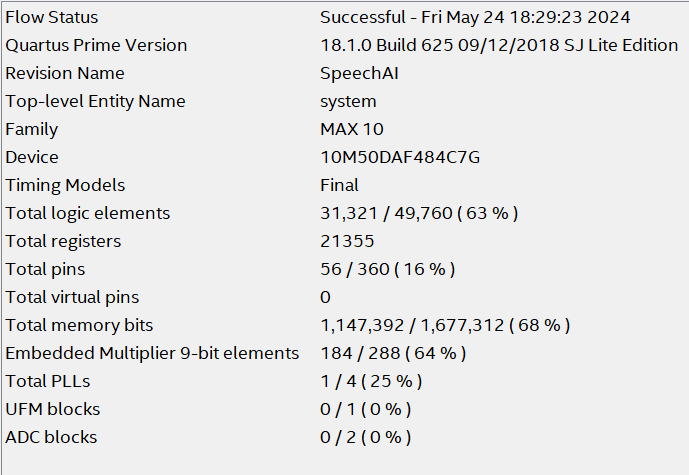
\includegraphics[width=0.7\textwidth]{zasoby1.png}
	\caption{Zużycie zasobów sprzętowych po podłączeniu wszystkich komponentów do procesora NIOS dla wersji systemu obsługującej SPI o~szybkości 67 MHz}
\end{figure}
\FloatBarrier %zatrzymanie przenoszenia rysunku

Projekt mieści się w~zaproponowanym układzie (\textit{MAX10} \textit{10M50}), zarówno pod względem zużycia bloków logicznych, pamięci BRAM, jak i~bloków DSP. System wykorzystuje jeden PLL, zarówno w~wersji z~dodatkową domeną zegarową w~celu osiągnięcia częstotliwości 67 MHz, która nie w~pełni zabezpiecza przed metastabilnością, jak i~w wersji 50 MHz-owej. Zużycie zasobów oscyluje wokół 64\%, a~pozostały zapas zasobów może posłużyć do dalszego rozwoju projektu, w~szczególności do dodawania nowych komponentów sprzętowych. Różnice między obiema wersjami są niewielkie.

Przy założeniu idei uniwersalnego systemu IoT dla algorytmu KNN, zaprojektowany system spełnia te wymagania. Ograniczając się do komponentów związanych ściśle z~rozpoznawaniem dźwięków (\textit{Signal\_Processor} oraz komponenty I/O), można uzyskać znaczący zapas bloków logicznych różnych typów. Można je wykorzystać do implementacji komponentów do pomiaru innych cech kluczowych, na przykład związanych z~rozpoznawaniem wideo, co również wymaga akceleracji sprzętowej.

Projekt pod względem zużycia zasobów należy więc ocenić pozytywnie, zarówno w~kontekście rozpoznawania dźwięków, jak i~jako uniwersalna platforma \textit{AI}.

\subsubsection{Parametry czasowe}

Po kompilacji sprawdzono również maksymalną bezpieczną częstotliwość dla danych domen zegarowych. Na rys. 7.3 i~7.4 zaprezentowano raport analizy czasowej dla temperatur 0°C i~85°C.

\begin{figure}[h]
	\centering
	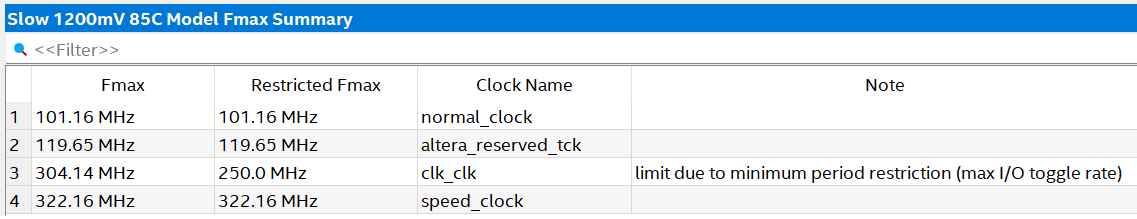
\includegraphics[width=1\textwidth]{85C.png}
	\caption{Maksymalna częstotliwość dla danych domen zegarowych dla wersji obsługującej SPI o~szybkości 67 MHz dla temperatury 85°C}
\end{figure}
\FloatBarrier %zatrzymanie przenoszenia rysunku

\begin{figure}[h]
	\centering
	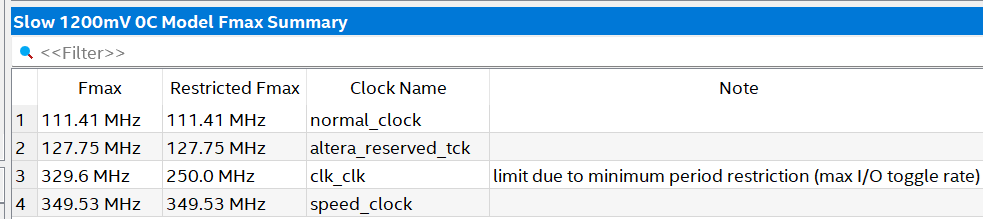
\includegraphics[width=0.8\textwidth]{0C.png}
	\caption{Maksymalna częstotliwość dla danych domen zegarowych dla wersji obsługującej SPI o~szybkości 67 MHz dla temperatury 0°C}
\end{figure}
\FloatBarrier %zatrzymanie przenoszenia rysunku

Układ FPGA, zarówno po dłuższej pracy (układ może się nagrzewać podczas intensywnego działania), jak i~w niskiej temperaturze, zachowuje parametry czasowe zgodne z~założeniami. Dla domeny \textit{normal\_clock}, czyli tej związanej z~procesorem i~komponentami, częstotliwość maksymalna wynosi powyżej 100 MHz (dla wysokich temperatur nieznacznie). Podobnie jest dla specjalnej domeny przeznaczonej do szybkiego odczytywania danych przez SPI - częstotliwość jest większa niż 200 MHz.

Parametry czasowe są zachowane również dla wersji 50 MHz. Nie wykorzystuje ona domeny \textit{speed\_clock}, gdyż dla tej częstotliwości nie ma potrzeby stosowania takiego rozwiązania. Rozwiązanie pod względem działania dla założonych częstotliwości zegara można uznać za wykonane poprawnie. Kompilator nie zgłasza problemów związanych z~konfliktami domen zegarowych dla wersji 67 MHz oraz innych problemów czasowych.

\subsection{Testowanie kluczowych komponentów}

Ze względu na złożoność systemu zdecydowano się na szczegółowe testowanie jedynie kluczowych komponentów, tj. \textit{SpeedSPI} oraz \textit{Signal\_Processor}.

Procesor sygnałowy testowano za pomocą testbencha. Stworzono kod w~języku \textit{Verilog}, który pozwala na generowanie ciągu próbek wystawianych na interfejs \textit{Avalon Stream}. Testbench wypisywał dane uzyskane po obliczeniu ich przez komponent. Wyniki porównywano z~wynikami generowanymi za pomocą skryptu w~środowisku \textit{Python}.

Wyniki były bardzo podobne, zazwyczaj różniły się o~około 2-3\%. Wynika to z~faktu, że obliczenia w~notacji \textit{fixed\_point} są mniej precyzyjne niż zmiennoprzecinkowe. Precyzja ta jest jednak nadal akceptowalna w~przypadku zastosowań w~sprzęcie embedded do pomiaru cech sygnału szumowego, gdzie sam szum ma większy wpływ na wyznaczenie transformacji niż wspomniany wcześniej błąd. Uznano więc, że \textit{Signal\_Processor} działa poprawnie.

Ze względu na bardzo dużą ilość ładowanych danych podczas analizy przez \textit{SpeedSPI}, jak na możliwości darmowej wersji programu \textit{ModelSim}, uznano, że testy zostaną wykonane w~sprzęcie. Test polegał na wykonaniu wykrycia wyrazu przez model referencyjny i~uzyskaniu profilu wykrytego wyrazu. Profil ten był wysyłany w~formie heksadecymalnego tekstu przez JTAG-UART do układu FPGA, tam ładowany do pamięci \textit{AI\_RAM}, po czym wykonywano komparację ze sprawdzeniem szczegółowych wyników kompilacji przez rejestry (szczególnie jeżeli chodzi o~wyniki punktowe).

Wyniki uzyskane podczas takich testów były identyczne jak te z~modelu referencyjnego, zarówno jeżeli chodzi o~samo wykrycie, jak i~wyniki punktowe. Testy takie wykonano dla wszystkich wyrazów. Uznano wówczas, że komponent \textit{SpeedSPI} nie wymaga dalszych testów.

Podsumowując, kluczowe komponenty działają prawidłowo i~nie znaleziono błędów, które utrudniałyby prawidłową detekcję wyrazów. Pozostałe komponenty sprawdzono podczas testów całego systemu, w~trakcie sprawdzania działania całej procedury rozpoznawania dźwięku.

\subsection{Testy czasu trwania procedury}
Po stworzeniu oprogramowania węzła rozpoczęto testy całej procedury wykrycia, od pomiaru cech kluczowych po wykrycie wyrazu. Poniżej przedstawiono raport programu węzła, który pokazuje, ile czasu zajmuje dana procedura.

\begin{lstlisting}
	Measure key features:
	Select loud fragment time: 89 ms
	Profile time: 3 ms
	Normalization time: 3 ms
	Time scaling time: 78 ms
	DMA time: 1 ms
	----
	Classifier working for database (10 MB -> 40 MB decompressed) 0 :
	351 ms
	Classifier working for database (10 MB -> 40 MB decompressed) 1 :
	351 ms
\end{lstlisting}

Można zauważyć, że procedury akcelerowane sprzętowo, takie jak wyznaczanie profilu i~normalizacja, są wykonywane znacznie szybciej od tych realizowanych przez program w~C. Zastosowany procesor jest stosunkowo wolny ze względu na brak pamięci \textit{cache} oraz układu mnożącego i~dzielącego, dlatego obliczenia są znacznie wolniejsze. Czas pomiaru cech kluczowych jest mniejszy od 200 ms uzyskanych dla modelu referencyjnego i~jest akceptowalny z~perspektywy użytkownika.

W kolejnym kroku klasyfikator sprawdza bazy danych. Aby porównać profil odebranego dźwięku z~jedną z~dwóch baz modelu, \textit{AI\_Comparer} potrzebuje 351 ms. Daje to sumaryczną szybkość ładowania danych z~4 kart wynoszącą 28,5 MB/s, co po dekompresji daje 114 MB/s. Cała procedura detekcji trwa 876 ms. Jest to czas mniejszy niż 1 sekunda, co jest akceptowalne z~perspektywy użytkownika.

Sytuacja wygląda nieco gorzej w~przypadku wersji 50 MHz. Zgodnie z~oczekiwaniami czas analizowania jednej bazy wydłużył się do 464 ms. Wówczas uzyskiwano szybkość danych zdekompresowanych na poziomie 86 MB/s, co dawało łączny czas detekcji dla 2 baz powyżej 1 sekundy (1,1 s). Mimo przekroczenia czasu akceptowalności, czas ten nie jest dużo większy niż założony limit, więc nadal można uznać go za akceptowalny. Z~tej przyczyny używanie tego systemu jest mniej komfortowe od wersji 66,7 MHz.

\subsection{Testy urządzenia}

Prototyp wykorzystano do testów w~terenie, aby sprawdzić, czy prawidłowo wykrywa wyrazy wymawiane w~jego otoczeniu. Przeprowadzono testy zarówno w~warunkach dużego hałasu, jak i~zupełnej ciszy.

Podobnie jak w~przypadku modelu referencyjnego, pewne wyrazy były wykrywane lepiej od innych. Niemniej jednak, wykrycia te były nieco gorsze niż dla implementacji w~środowisku \textit{Python}. Niektóre wyrazy były wykrywane bardzo rzadko (raz na 2-3 próby, co stanowiło poniżej 50\%), inne zaś były prawie zawsze (19 na 20 prób, co dawało 95\%).

\begin{figure}[h]
	\centering
	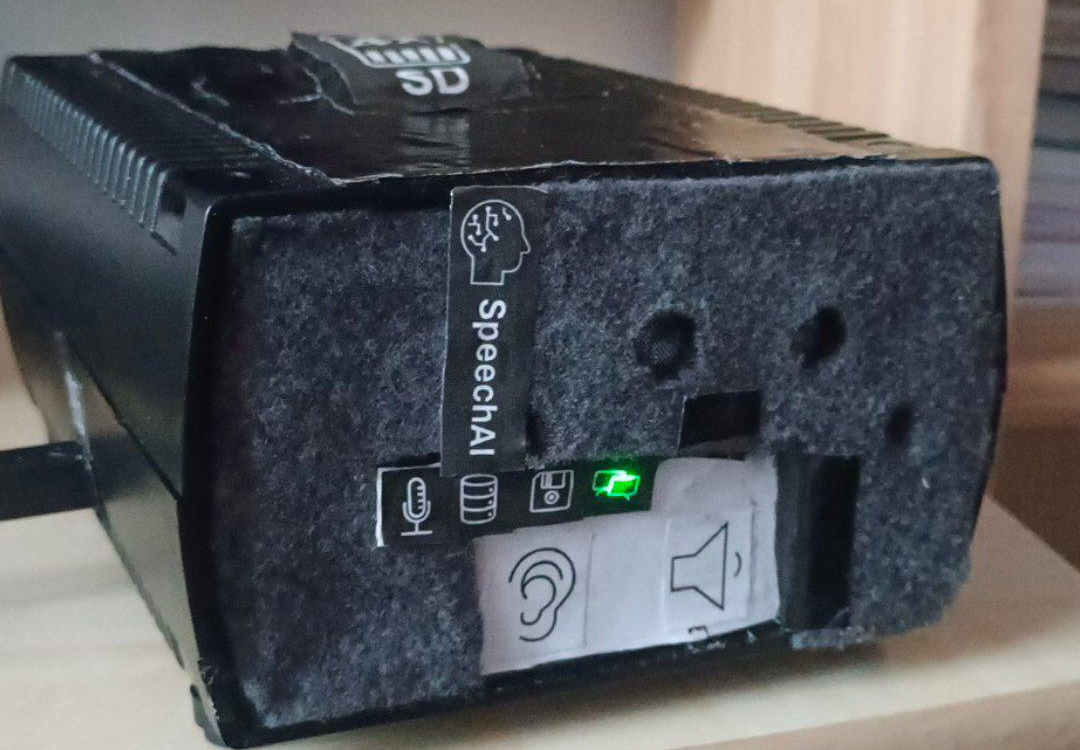
\includegraphics[width=0.5\textwidth]{prototyp.png}
	\caption{Zdjęcie prototypu w~obudowie}
\end{figure}
\FloatBarrier %zatrzymanie przenoszenia rysunku



System nadal spełniał założenia wykrywania wyrazów dla określonej małej puli wyrazów. Czas oczekiwania na detekcję wyrazu wynosił około 1 sekundy, co jest akceptowalne z~perspektywy użytkownika oraz ograniczeń kanału komunikacyjnego, jakim jest ludzka mowa. Różnice między modelem referencyjnym a~urządzeniem wynikają z~zastosowania notacji fixed-point zamiast zmiennoprzecinkowej oraz kopiowania pamięci przez \textit{AI\_DMA}, które ograniczają precyzję.

\begin{figure}[h]
	\centering
	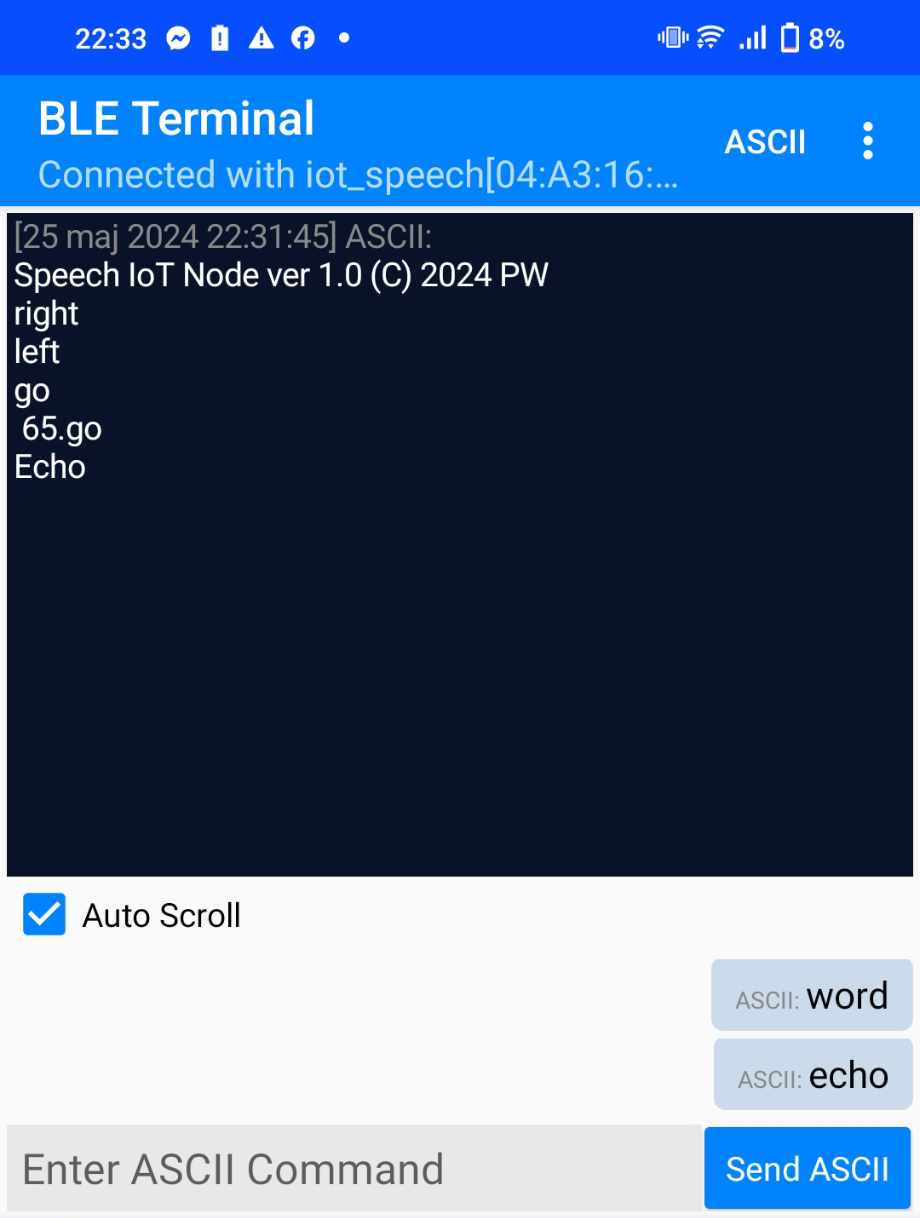
\includegraphics[width=0.5\textwidth]{komunikajca.png}
	\caption{Zrzut ekranu z~programu \textit{BLE Terminal} pokazujący działanie komunikacji między węzłem a~innym urządzeniem}
\end{figure}
\FloatBarrier %zatrzymanie przenoszenia rysunku

Wyrazy, po prawidłowym przejściu przez procedurę dialogową, były przesyłane do urządzenia zewnętrznego. Jako bramkę \textit{BLE} użyto, na potrzeby testu, telefonu z~obsługą standardu \textit{Bluetooth} oraz aplikacją \textit{BLETerminal}. Wyniki testu przedstawiono na rys. 7.6.

Po uruchomieniu węzła wyświetla się komunikat o~jego uruchomieniu (\textit{Speech IoT Node ver 1.0 (C) 2024 PW}), a~następnie kolejne wyrazy, które przeszły procedurę walidacji przez system dialogowy. Z~węzłem można było również komunikować się za pomocą komend takich jak \textit{echo} czy \textit{word}.

Rozwiązanie działało stabilnie podczas testów, cały czas wykrywając wyrazy, pod warunkiem, że użytkownik znajdował się w~pobliżu węzła, aby czujnik odległości go wykrył, oraz wyraźnie wymawiał komendę lub hasło wywoławcze (\textit{Sheila}). Uznano, że całą implementację prototypu należy ocenić pozytywnie.


\subsection{Porównanie z~innymi rozwiązaniami}

Zgodnie z~rozdziałem 3.4, podobnym rozwiązaniem do wykonanego w~ramach tej pracy jest dostępny w~najnowszych platformach \textit{ARM Cortex - M7} \textit{DS-CNN KWS}. Rozwiązanie to jest znacząco szybsze od zaprezentowanego przez autora – czas pomiaru cech kluczowych oraz komparacji z~jedną bazą wynosi ponad 600 ms (w porównaniu z~12 ms dla ARM). Trzeba zaznaczyć, że największe obciążenie jest związane z~zadaniami liczonymi w~programie w~C (wybór głośnego fragmentu i~skalowanie w~dziedzinie czasu). Procesy akcelerowane sprzętowo – normalizacja i~wyznaczanie profilu – są znacznie szybsze, około 3 ms.

Problematyczna jest także sama klasyfikacja związana z~wolnymi nośnikami danych i~dużą bazą. Baza zastosowana w~tym projekcie ma 10 MB po skompresowaniu (czyli przed kompresją miała 40 MB). Modele stosowane w~\textit{KWS} często mają mniej niż megabajt. Procesory z~rodziny \textit{ARM} działają na zegarach o~częstotliwościach około 400 MHz, podczas gdy rozwiązanie z~tej pracy – na 100 MHz \cite{tinyML}. Zegar tam jest więc 4 razy szybszy.

Mimo że rozwiązanie jest znacznie wolniejsze, to nadal czas detekcji wyrazu jest akceptowalny (około 1 sekundy). Wprowadzenie pewnych zmian w~projekcie powinno sprawić, że rozwiązanie zbliży się do wyniku uzyskanego przez \textit{KWS}. Eksperymentowano podczas opracowywania projektu z~bazami czterokrotnie zmniejszonymi, co skróciło czas wyszukiwania przez bazę do 87 ms. Zakładając odczyt za pomocą szybszego interfejsu niż 67 MHz SPI, np. gdyby karty czytano z~szybkością 25 MB/s (na tyle, ile maksymalnie pozwala obecna implementacja \textit{AI\_Comparer}), uzyskano by czas około 30 ms na porównanie całej bazy. Jest to wynik nadal większy niż ten w~procesorze ARM (szczególnie że ten czas uwzględnia również pomiar cech kluczowych), ale biorąc pod uwagę, że procesory ARM mają 4-krotnie szybszy zegar, daje to wynik satysfakcjonujący. Czas obliczania profilu i~jego normalizacji łącznie wynosi około 7 ms, co jest dobrym czasem. Należałoby przemyśleć akcelerację pozostałych procesów, np. skalowania w~dziedzinie czasu.

Zużycie pamięci operacyjnej przez urządzenie jest bardzo podobne do tego uzyskanego w~rozwiązaniu opisanym w~rozdziale 3.4 – program łącznie używał 81 kB pamięci RAM, podczas gdy rozwiązanie od ARM około 70 kB. Nie są to wartości znacznie rozbieżne. Podczas analizy założono pesymistycznie, że cała pamięć wolna dla stosu może zostać użyta, co jest mało prawdopodobne, więc zużycie jest prawdopodobnie mniejsze.

\subsection{Dalsze prace}

Projekt ma wysoki potencjał rozwojowy, uwzględniając szczególnie dzisiejszy intensywny rozwój różnych gałęzi zarówno internetu rzeczy, jak i~sztucznej inteligencji.

W przyszłości można by zastanowić się nad zmianą nośnika danych oraz standardu komunikacji. Aby uzyskać stosunkowo niewielką prędkość 7,5 MB/s odczytu z~jednego nośnika, konieczne było stosowanie bardzo ryzykownych zabiegów. Karty SD mają standard komunikacji 4-pinowej, ale uzyskanie dostępu do niego wymaga wykupu licencji produkcyjnej. Z~perspektywy studenta oraz uczelni jest to zbędny wydatek. Dobrą alternatywą byłyby pamięci flash komunikujące się po interfejsie QSPI (interfejs SPI z~4-bitową linią komunikacyjną). Wtedy nawet stosując częstotliwość 50 MHz, uzyskujemy prędkość do 25 MB/s dla jednej takiej pamięci, co uwzględniając proces dekompresji, znacznie przyspieszyłoby wykrywanie wyrazów. Jak wcześniej wspomniano, najpoważniejszym wąskim gardłem jest czytanie danych z~nośnika, a~nie samo działanie klasyfikatora. Myśląc o~jeszcze większych szybkościach, można zdecydować się na karty \textit{Compact Flash} \cite{CF}.

Warto byłoby dokonać bardziej szczegółowych testów, wykonać testbenche wszystkich komponentów. Dawałoby to większą pewność, że cały system działa poprawnie. Warto byłoby opracować lepszą metodę trenowania modelu. W~projekcie zastosowano wybranie pierwszych 256 nagrań na podstawie kolejności, w~jakiej podane zostały przez system plików. Korzystnym byłoby opracowanie systemu wyboru nagrań, aby pozbyć się różnych nagrań o~niskiej jakości, co usunęłoby z~modelu elementy zmniejszające precyzję wykryć. Można by wówczas przy użyciu mniejszej liczby nagrań uzyskać taki sam efekt, jaki jest obecnie. Dodatkowo warto przeanalizować możliwość przeniesienia do komponentów w~układzie FPGA innych algorytmów, np. skalowania w~dziedzinie czasu.

Komponenty \textit{AI\_Comparer} oraz \textit{Signal\_Processor} należałoby poprawić pod względem uzyskania większej potokowości. Trzeba wymienić zewnętrzny komponent FFT na własny, wykonany pod kątem współpracy z~interfejsem \textit{Avalon Stream}. W~wielu miejscach zastosowano dla uproszczenia procesu projektowania automaty stanów, co jest rozwiązaniem nieefektywnym w~przypadku implementacji strumieniowych. O~ile dane zadanie tego nie wymaga – a~w~większości sytuacji nie ma takiej konieczności – warto byłoby zamienić je na szybsze alternatywy. Pozwoli to pracować z~jeszcze większymi szybkościami, umożliwiając szybsze wykrywanie wyrazów i~zbliżenie się do wyników uzyskiwanych przez rozwiązanie \textit{ARM}.